%%% Inicio del documento se define la clase y
%%%tesisupiita )Tesis: UPIITA-IPN
%Copyright (C) 2017 Juan Carlos Guzm�n Salgado
%% Griselda S�nchez Otero
%%% propiedades generales
\documentclass[letterpaper,11pt]{upiita}
%%%%%%%%%%%%%%%%%%%%%%%%%%%%%%%%%%%%%%%%%%%%%%%%%%%%%%%%%%%%%%%%%%%%%%%
%%%%%%%%%%%%%%%%%%%%%%%%%%%%%%%%%%%%%%%%%%%%%%%%%%%%%%%%%%%%%%%%%%%%%%%
%%%%%%%%%Paquetes utilizados%%%%%%%%%%%%%%%%%%%%%%%%%%%%%%%
%%%%%%%%%%%%%%%%%%%%%%%%%%%%%%%%%%%%%%%
\usepackage{upiitatesis}
\usepackage{float}
\usepackage{makeidx}
\usepackage{amsfonts}
\usepackage{amsmath}
\usepackage{mathrsfs}
\usepackage{eucal}
\usepackage{mathrsfs}
\usepackage{graphicx}
\usepackage{lettrine}
\usepackage[pdftex=false,colorlinks=true]{hyperref}
\usepackage[spanish]{babel}
\usepackage[latin1]{inputenc}
\usepackage[Sonny]{fncychap}
\usepackage{fancyhdr}
\usepackage{subfigure}
\usepackage{layout}
\usepackage{textcomp}
\usepackage{bbding}
\usepackage{ifthen}
\usepackage{pifont}
\usepackage{romanidx}
\usepackage{titlesec}
\usepackage{titling}
\usepackage{booktabs}
\usepackage{multirow}
\usepackage[dvipsnames]{xcolor}
\usepackage{colortbl}
%%Propiedades adicionales
%%%%%%%%%genera secci�n de �ndice %%%%%%%%%
\makeindex
%%%%%%%%%%%%%%%%%%%%%%%%%%%%%Inicio de documento}}}
\begin{document}
%%%%%%%% Inicio de Secci�n de preliminares numeraci�n con n�meros romanos%%%%
\frontmatter
%%%%%%%%%%%%%  Datos de la Portada y acta
\title{Rodamientos Magn�ticos H�bridos}
\unidad{\Upiita}
\materia{Trabajo Terminal II}
\academia{Mecatr\'onica}
\degree{Ingeniero en Mecatr\'onica}     %%%%%%%%%%%%%grado
\degreemonth{MAYO}                     %%%%%%%%%%mes
\degreeyear{2017}                       %%%%%%%%%%a�o
%%%%%%%%%%%%  Nombre del Presidente y Secretario del jurado
\Presidente{M. en C. Alfonso Campos V�zquez}
\Titular{M.en C. Griselda S�nchez Otero}
%%%%%%%%%%%%%%%%%%%%%%% Datos del autor%%%%%%%%%%%
%%%%%%%%%%%%%%%%%%%%%%%%%%%%%%%%%%%%%%%%%%%%%%%%%
%%para varios asesores (m�ximo 4) y autores (alumnos) dejar el campo en blanco de los que no deban aparecer
%%%%%%%%%% Cuando el n�mero de asesores=1 s�lo se toma en cuenta la variable alumnoa,
%%                                     =2 se toman alumnoa y asesorb, etc
%%%%%%%%%%%%%%%%%%%%%%%%%%%%%
\nalumnos{3}
%%%%%%% dependiendo del numero de alumno dejar vac�o el campo de alumnoX, nunca eliminar o comentar la l�nea
\alumnoa{Omar Alejandro Bejarano Montiel}
\alumnob{Oscar Enriquez Ramirez}
\alumnoc{Manuel Enrique Limones Urbina}
%\alumnod{Giovanni Karol}
%%%%%%%%%% n�mero de asesores 1= solo se toma en cuenta la variable asesora, 2= se toman asesora y asesorb
\nasesores{1}
%%%%%%% en caso de un �nico asesor dejar vac�o el campo de asesorb, nunca eliminar o comentar la l�nea
\asesora{M. en C. �lvaro Gordillo Sol}
%\asesorb{Dr. Johannes Carolus}
%\asesorc{Dr. Ivan Karurosu}
%%creacion de p�ginas
\portada
\acta
\dedicatoria              %%%modificar archivo dedica.tex
\agradecimientos          %%%modificar archivo agradece.tex
\tableofcontents
\listoffigures
\listoftables
\chapter{Resumen}

\textbf{\Large Rodamientos Magn�ticos H�bridos}\\



\textbf{Palabras Clave:}  Rodamientos, levitaci\'on magnetica, electroimanes, control por variable estado, sensor capacitivo, simulaci\'on magnetica, Areas funcionales, materiales, ferromagn\'eticos, PDS.     \\

\textbf{Resumen:}

...

\textbf{Abstract:}

...
               %%%modificar archivo Resumen.tex
\chapter{Nomenclatura}

\textbf{Lista de nomenclaturas:}\\


\begin{tabular}{ll}
	RMH\hspace{3cm} & Rodamientos Magn\'eticos H\'ibridos\\
	RMA\hspace{3cm} & Rodamientos Magn\'eticos Activos\\
	RMP\hspace{3cm} & Rodamientos Magn\'eticos Pasivos\\
	POM\hspace{3cm} & Polioximetileno \\
	PA\hspace{3cm} & Poliamida\\
	MCCE\hspace{3cm} & Modulo de Compensaci\'on de Cargas Est\'aticas\\
	PDS\hspace{3cm} & Product Design Specifications\\ 
	EA\hspace{3cm} & Electroiman Axial\\
	ER\hspace{3cm} & Electroiman Radial\\
	IP\hspace{3cm} & Iman Permanente\\
	SDC\hspace{3cm} & Sensor de Desplazamiento Capacitivo\\
\end{tabular}

          %%%modificar archivo Nomenclatura.tex
\chapter{Simbolog\'ia}


\begin{tabular}{ll}
	$H$\hspace{3cm} & Campo magn\'etico \\
	$B$\hspace{3cm} & Inducci\'on magn\'etica\\
	$\mu_0$\hspace{3cm} & Permeabilidad magn\'etica del vac\'io \\
	$\phi$\hspace{3cm} & Flujo magn\'etico\\
	$M$\hspace{3cm} & Magnetizaci\'on\\
	$m$\hspace{3cm} & Momento magn\'etico\\
	$\mu$\hspace{3cm} & Permeabilidad del material\\ 
	$X$\hspace{3cm} & Susceptibilidad\\
	$\mu_r$\hspace{3cm} & Permeabilidad relativa\\
	$M_0$\hspace{3cm} & Magnetizaci\'on de saturaci\'on\\
	$M_s$\hspace{3cm} & Saturaci\'on t\'ecnica\\
	$B_R$\hspace{3cm} & Inducci\'on magn\'etica residual\\
	$M_R$\hspace{3cm} & Magnetizaci\'on residual\\
	$H_c$\hspace{3cm} & Coercitividad\\
	$\eta$\hspace{3cm} & Fuerza magnetomotriz\\
	$R$\hspace{3cm} & Reluctancia\\
	$\epsilon$\hspace{3cm} & Fuerza electromotriz\\
	$W_m$\hspace{3cm} & Energ\'ia magn\'etica\\
	$F_m$\hspace{3cm} & Fuerza magn\'etica \\
	$\mu_m$\hspace{3cm} & Permeabilidad magn\'etica\\	
	$M_o$\hspace{3cm} & Matriz de observabilidad\\
	$M_c$\hspace{3cm} & Matriz de controlabilidad\\
	$K$\hspace{3cm} & Matriz de ganancias\\
	
	\\
\end{tabular}

            %%%modificar archivo Simbologia.tex
\chapter{Objetivos}

\section*{Objetivo general}
Dise�ar y simular un sistema de rodamientos magn�ticos capaz de operar en condiciones de carga est�tica.

\section*{Objetivos Particulares.}

{\setlength{\parindent}{0pt}Trabajo Terminal I:}
\begin{enumerate}
\addtolength{\itemsep}{0pt}
\item Obtener el dise�o conceptual del rodamiento magn�tico h�brido.
\item Obtener el dise�o conceptual del rodamiento magn�tico h�brido.
\item Seleccionar el material ferromagn�tico para el n�cleo de los electroim�nes. 
\item Calcular la secci�n transversal de los electroim�nes.
\item Obtener la geometr�a y dimensiones de los rodamientos activos radial y axial.
\item Validar el punto de operaci�n del electroim�n mediante simulaci�n.
\item Dise�ar un electrodo de alta sensitividad para el rango de operaci�n.
\item Dise�ar un dispositivo para la retracci�n del im�n permanente. 
\item Proponer un circuito de adquisici�n y control. 
\end{enumerate}
\hfill \break

{\setlength{\parindent}{0pt}Trabajo Terminal II:}
\begin{enumerate}
\addtolength{\itemsep}{0pt}
\item Obtener un modelo de electroim�nes que integre los efectos del flujo marginal.
\item Realizar las simulaciones de la fuerza magn�tica ejercida por los electroim�nes y el im�n permanente.
\item Obtener el modelo din�mico del sistema.  
\item Comparar algunos esquemas de control para la estabilizaci�n del sistema.
\item Dise�o del circuito de potencia de los electroim�nes. 
\item Estimar los l�mites de operaci�n del rodamiento con base en las simulaciones.
\end{enumerate}             %%%modificar archivo objetivos.tex
%%%%General
%%%%Espec�ficos
\chapter{Introducci\'on}

El desarrollo de nuevas investigaciones y tecnolog�as han permitido que la industria busque nuevas y mejores formas de llevar a cabo sus procesos productivos, lo que requiere; entre otras cosas, de transformar y actualizar la maquinaria y equipo que utilizan con el prop�sito de volverlos m�s eficientes y aumentar su productividad.
En este aspecto se han realizado numerosos avances y descubrimientos, como pueden ser el uso de fuentes de energ�a m�s limpias y eficientes, la implementaci�n de nuevos materiales m�s ligeros y resistentes, y por supuesto, el reemplazo de algunos componentes y dispositivos por otros m�s avanzados.

Gran parte de la maquinaria industrial posee elementos de tipo rotativo, los cuales requieren el uso de dispositivos denominados cojinetes, tambi�n conocidos como rodamientos o baleros. Estos suelen situarse entre dos componentes de la m�quina con un eje de rotaci�n com�n, facilitando el movimiento de giro de un componente con respecto al otro y reduciendo la fricci�n de los diferentes elementos m�viles. Los rodamientos son a su vez, un punto de apoyo para dichos ejes o �rboles. 

Adem�s de ser capaces de disminuir la fricci�n, de manera general los rodamientos deben cumplir con algunas caracter�sticas particulares como son: disminuir las vibraciones, operar de manera silenciosa y poseer una prolongada vida �til. Sin embargo, los distintos sectores industriales suelen establecer sus propios requisitos espec�ficos con base en determinados entornos operativos o aplicaciones particulares, entre los que podemos mencionar: resistir grandes cambios de temperatura, humedad, suciedad, operar en medios agresivos como soluciones �cidas o alcalinas, soportar altas velocidades e incluso ser aptos para el contacto con alimentos  \cite{cite_1}.

Es por ello que dentro de los rodamientos existe una gran variedad de configuraciones, materiales y modos de operaci�n que puedan satisfacer esta demanda de necesidades.

\section*{Clasificaci�n de Cojinetes y Rodamientos}

Los cojinetes se clasifican principalmente en dos grandes grupos: cojinetes de deslizamiento (o de fricci�n) y antifricci�n (rodamientos). Los cojinetes de deslizamiento consisten b�sicamente en un par de casquillos conc�ntricos que giran en contacto directo uno con el otro realiz�ndose un deslizamiento por fricci�n, procurando que esta sea la menor posible; la disminuci�n de la fricci�n depende de los materiales con los que est�n fabricados y del uso de alguna pel�cula lubricante \cite{cite_2}. 

Por su parte, los cojinetes antifricci�n (rodamientos) comprenden una clasificaci�n m�s extensa debido a su complejidad estructural, en comparaci�n a los cojinetes de deslizamiento. Entre los principales podemos encontrar: por la direcci�n de la carga que soportan (axial, radial, angular o mixta, y lineal), seg�n su rigidez (r�gidos y pivotantes) y por el tipo de cuerpo rodante (de bolas, rodillos, agujas, c�nicos, etc.)\cite{cite_3}. 

El rozamiento por rodadura generado por los rodamientos es mucho menor que el de los cojinetes de deslizamiento, y es por ello que presentan una serie de ventajas m�s frente a la utilizaci�n de casquillos que incluye mayor velocidad admisible, menor temperatura de funcionamiento, mayor capacidad de carga, menor desgaste, facilidad de recambio y disminuci�n en los costos de mantenimiento. 

A pesar de todo esto, existen algunas aplicaciones para las cuales se deben buscar alternativas a estos dispositivos mec�nicos, particularmente las que est�n relacionadas con m�quinas rotativas de alta velocidad donde se incrementan de manera considerable las p�rdidas mec�nicas, las cuales est�n asociadas al rozamiento y a las vibraciones mec�nicas. Ante este problema surge un tipo de rodamiento que opera por medio de la suspensi�n magn�tica, conocidos como rodamientos magn�ticos.  

\newpage

\section*{Rodamientos Magn�ticos}
%\label{sec:intro:motivation}
%\addcontentsline{toc}{section}{Rodamientos Magn�ticos}

Como ya se mencion� anteriormente, los rodamientos magn�ticos son una excelente alternativa para su uso en m�quinas rotativas de alta velocidad, ya que presentan m�ltiples ventajas frente a los rodamientos tradicionales, como una mayor velocidad de giro, no requieren de un sistema de lubricaci�n ya que operan sin contacto, por lo que adem�s no producen part�culas de desgaste y debido a su baja rigidez son capaces de compensar las vibraciones mec�nicas haci�ndolos silenciosos. Todo esto se traduce en una disminuci�n de los costos de mantenimiento y prolongaci�n de la vida �til del sistema.

El potencial que poseen para generar muy pocas p�rdidas y alcanzar mayores velocidades los hace ideales para aplicaciones industriales como centrifugadoras de alta velocidad, volantes inerciales, compresores y turbinas de alto r�gimen de revoluciones, por mencionar algunas. 
Los rodamientos magn�ticos cuentan, a su vez, con una clasificaci�n que viene en funci�n de dos principales factores: de acuerdo a la naturaleza de su fuerza, que puede ser de Reluctancia o de Fuerza de Lorentz, o m�s com�nmente de acuerdo a la fuente generadora del campo magn�tico (Pasivos, Activos e H�bridos)\cite{cite_4}. 

Los pasivos carecen de alimentaci�n externa y emplean imanes permanentes para generar los campos magn�ticos de levitaci�n, mientras que los activos utilizan electroimanes y requieren de una fuente de alimentaci�n externa y de un sistema de control. Por su parte, los h�bridos emplean imanes permanentes para crear un campo base de levitaci�n mientras que el resto del campo es generado por electroimanes.

A pesar de que la mayor�a de los usos que se le dan a los rodamientos magn�ticos pertenecen al sector aeroespacial, naval, generador de energ�a y otras aplicaciones de alta demanda, tambi�n es posible aprovecharlos en otro tipo de maquinaria m�s comercial pudiendo explotar al m�ximo sus beneficios. 

\newpage

\section*{Antecedentes}
\subsection*{Investigaci�n y Desarrollo de Rodamientos Magn�ticos}

Pese a las m�ltiples ventajas que presentan, los rodamientos magn�ticos no est�n exentos de algunos problemas que pueden dificultar su desarrollo e implementaci�n en los sistemas industriales, entre los que podemos destacar el alto consumo energ�tico que generan.\par
Ante este problema se hicieron varias investigaciones cuyas soluciones pueden clasificarse en dos tipos: el dise�o de algoritmos para minimizar las corrientes en los electroimanes y el uso de imanes permanentes para proveer un campo magn�tico base para la levitaci�n.\par
La investigaci�n realizada en \cite{cite_5} se trata de una validaci�n experimental en donde primero se dise�a y construye un prototipo de pruebas que emula el comportamiento de un rodamiento magn�tico activo de un grado de libertad, y segundo se realizaron pruebas para evaluar el desempe�o del controlador inteligente en comparaci�n con un controlador est�ndar de polarizaci�n fija.\par
Este equipo consiste en un eje r�gido capaz de balancearse libremente sobre un punto de apoyo colocado debajo de su centro de masa. La posici�n angular de este eje es controlada mediante electroimanes fijados a los extremos de este. A pesar su simplicidad este equipo incorpora todas las no linealidades t�picas de un rodamiento magn�tico activo, y la din�mica del sistema es ideal para evaluar el desempe�o de los controladores.\par
En \cite{cite_6} una estrategia de control de corriente de polarizaci�n variable es presentada con el fin de minimizar la energ�a consumida sin alterar el desempe�o din�mico del sistema. El modelado parte de un RMA de 2 polos sobre el cual se propone un controlador lineal y un observador de estados para la estimaci�n de estados. Una vez obtenido el modelo del sistema se calcula de manera anal�tica la corriente �ptima para la estabilizaci�n del sistema y obtener el controlador.\par
Como resultado este controlador propuesto fue capaz de reducir el consumo en un 73\%, se estabiliz� la posici�n de rotor en el centro del rodamiento con un error de estado estable nulo y se presentaron vibraciones 60\% menores comparadas con un controlador de polarizaci�n fija.

\newpage

\subsection*{Rodamientos Magn�ticos en la Industria}

En la actualidad los sistemas de rodamientos magn�ticos tienen m�ltiples aplicaciones dentro del campo industrial, y aunque la mayor�a cuenta con adaptaciones acorde a la maquinaria en la que se utilizar�, poseen una arquitectura y un modo de funcionamiento similar.

La empresa FAG�, filial de Schaeffler Group, ha desarrollado un sistema de rodamiento magn�tico activo que denominan como modular. Su sistema de control y de electr�nica de potencia es capaz de ajustarse a ciertos par�metros definidos por el usuario acorde a los requerimientos de operaci�n, y su dise�o permite una f�cil integraci�n en la arquitectura de la m�quina.

Otra de las ventajas que posee es que pr�cticamente no existen restricciones de velocidad y puede soportar pesos de eje de m�s de 9 toneladas. Cuenta con un sistema de apagado de seguridad que previene da�os a la m�quina y gracias a los cojinetes de respaldo que integra tambi�n la protege en caso de una interrupci�n en el suministro de energ�a que conduzca al fallo del cojinete magn�tico. A su vez sirven de apoyo para el rotor cuando los cojinetes magn�ticos est�n apagados \cite{cite_7}.
Sin embargo, ya que se trata de una empresa especializada este producto resulta altamente costoso, adem�s de que �nicamente est�n orientados a aplicaciones de alta demanda y cargas muy grandes.

Por su parte la empresa YORK� Navy Systems de Johnson Controls, quien desarroll� uno de los primeros sistemas de rodamientos magn�ticos para su uso en enfriadores centr�fugos en embarcaciones de grado militar, ha sido capaz de aplicar esta tecnolog�a en enfriadores comerciales, logrando alargar el tiempo de vida de la m�quina disminuyendo el n�mero de partes m�viles y removiendo los sistemas de lubricaci�n tradicionales. Esto se traduce en una reducci�n significativa de los costos de mantenimiento. Utiliza un sistema de velocidad variable el cual ralentiza el motor cuando el enfriador est� funcionando en condiciones fuera de dise�o, adem�s de mejorar la fiabilidad durante el arranque al asegurar que la corriente de entrada nunca supere el 100\% de los amperes de carga completa. Y finalmente gracias a las vibraciones casi indetectables, el ruido se reduce casi por completo \cite{cite_8}. 

Aunque han logrado ampliar esta tecnolog�a para aplicaciones comerciales e industriales fuero del �mbito militar, este sistema est� desarrollado casi exclusivamente para plantas de enfriamiento y aire acondicionado, por lo que no es capaz de usarse y adaptarse a otro tipo de sistemas.

Por otro lado, la empresa Synchrony� ha realizado grandes avances en cuanto a tecnolog�a de rodamientos magn�ticos se refiere. Han logrado disminuir el tama�o de la unidad de control eliminando o miniaturizado algunos componentes como los convertidores A/D y D/A, los amplificadores de potencia y la interfaz de comunicaciones, y el uso de contadores de alta velocidad para la se�al de posici�n. Una de las innovaciones m�s importantes ha sido el desarrollo de sensores de posici�n que pueden ser integrados directamente en los electroimanes.

Han reducido dram�ticamente el tama�o de los rodamientos magn�ticos axiales y radiales mediante el uso de nuevas e innovadoras t�cnicas de dise�o y manufactura. Todas estas modificaciones han reducido en general la complejidad del sistema \cite{cite_9}.
Sin embargo, la disponibilidad de productos es baja, y solamente ofrecen servicio a un n�mero muy limitado de pa�ses.

\newpage

\section*{Planteamiento del problema}

En la actualidad, los avances tecnol�gicos tienden hacia el desarrollo de sistemas m�s peque�os, veloces, eficientes, y con un menor consumo de energ�a y m�nimo mantenimiento. Estas cualidades adquieren gran importancia dentro del �mbito industrial, donde sus beneficios impactan directamente en el desarrollo de mejores m�quinas y dispositivos, como motores, compresores, enfriadores, sistemas de centrifugaci�n y sistemas de transmisi�n, por mencionar algunos.

Gran parte de estos y otros dispositivos rotativos no son capaces de alcanzar altas velocidades debido al rozamiento y a las vibraciones que se producen en los ejes y �rboles de transmisi�n; entre m�s revoluciones alcance, mayor ser� el calor generado por la fricci�n, y las p�rdidas mec�nicas incrementan de manera considerable. 

Pese a que los rodamientos suprimen algunas de las desventajas propias de los cojinetes de deslizamiento, a�n presentan algunos inconvenientes para su uso en maquinaria de alta velocidad; estos problemas abarcan principalmente su sensibilidad a la contaminaci�n debido a la generaci�n de part�culas de desgaste, una baja resistencia a las cargas de impacto , generaci�n de cargas fluctuantes  (vibraciones), mayor nivel de ruido ac�stico, y aunque el coeficiente de rozamiento es bajo, los materiales contin�an funcionando en contacto directo, lo que provoca un incremento en las temperaturas de operaci�n.Para hacer frente a estas desventajas es necesario considerar el uso de un nuevo tipo de rodamientos que reemplace a los convencionales, por lo que un sistema de rodamientos magn�ticos resulta en una buena alternativa que atrae importantes beneficios. 

Dado que los rodamientos magn�ticos trabajan sin contacto directo con los elementos que soportan, pueden disminuir de manera considerable las p�rdidas mec�nicas debido a la supresi�n del rozamiento de los cojinetes de apoyo y otras partes m�viles. Esto permite reducir la potencia necesaria de los motores e incrementar la eficiencia, y son capaces de compensar las vibraciones y cargas fluctuantes. La reducci�n de las p�rdidas implica tambi�n que las temperaturas de operaci�n sean menores, y en algunos casos esto permite que no sea necesario el uso de equipos de refrigeraci�n adicionales. 

Los rodamientos magn�ticos no requieren del uso de lubricantes, lo que los hace ideales para m�quinas que trabajan en ambientes con temperaturas extremas, en condiciones de vac�o, que se encuentren en contacto con sustancias corrosivas o cualquier m�quina que no tolere la contaminaci�n por las part�culas de desgaste o de los mismos lubricantes, adem�s elimina la necesidad de implementar sistemas de lubricaci�n extras.

Todos estos beneficios implican una reducci�n significativa de los costos inherentes al mantenimiento, relacionados principalmente al reemplazo de piezas debido al desgaste, adem�s de la eliminaci�n de sistemas adicionales de refrigeraci�n y lubricaci�n y a una necesidad de mantenimiento peri�dico menor \cite{cite_10}. 

A pesar de las m�ltiples ventajas que ofrece este tipo de sistemas, no se ha logrado ampliar su uso dentro de la industria debido principalmente a que presentan otro tipo de desventajas que no se encuentran en los cojinetes y rodamientos, como su accesibilidad limitada, un precio m�s elevado, la necesidad de contar con un sistema de control y la posibilidad de fallas en el sistema el�ctrico, adem�s de que en el caso de los rodamientos magn�ticos activos el consumo el�ctrico suele ser elevado.

Es por eso que en este sentido se opt� por el desarrollo de rodamientos magn�ticos de funcionamiento h�brido, ya que al utilizar un campo base otorgado por los imanes permanentes, el consumo el�ctrico de los electroimanes es menor. Este proyecto tendr� como finalidad desarrollar un sistema que pueda brindar una alternativa a los rodamientos magn�ticos tradicionales en proyectos relacionados con el desarrollo de maquinaria y equipo industrial.

\newpage

\section*{Descripci�n de los Cap�tulos}

Este documento se divide principalmente en cuatro cap�tulos:

\begin{enumerate}
\item Marco te�rico. 
\item Dise�o conceptual.
\item Dise�o detallado.
\item Validaci�n y an�lisis de resultados.
\end{enumerate}

El Marco te�rico tiene como finalidad describir los conocimientos fundamentales aplicados al proyecto durante el desarrollo del mismo. Entre los m�s importantes est�n la comprensi�n de los fen�menos de electricidad y magnetismo, el control de sistemas lineales y discretos, los filtros de Kalman, entre otros. A su vez, refuerza y repasa los conocimientos sobre electr�nica y conceptos de dise�o mecatr�nico (PDS y an�lisis funcionales) para permitir una mejor vinculaci�n entre los elementos matem�ticos de control y el fen�meno de levitaci�n magn�tica.

El objetivo del cap�tulo del Dise�o conceptual es describir la importancia del desarrollo te�rico de este proyecto, as� como el impacto industrial que tiene. Marca las acotaciones de las especificaciones sobre las que se dise�� el rodamiento, y establece a grosso modo la morfolog�a del prototipo. Define tambi�n las �reas funcionales sobre las que se trabaj� durante la gestaci�n del proyecto, y muestra un an�lisis morfol�gico para determinar de forma general un dise�o apropiado de qu� presentaci�n final tendr�a el prototipo.

El Dise�o detallado describe el desarrollo de cada �rea funcional a detalle bas�ndose en los procedimientos descritos en el cap�tulo 1 y retoma los bocetos del dise�o conceptual en el cap�tulo 2. Esto con el fin de que para el final de este cap�tulo, se obtenga una simulaci�n que cumpla los requerimientos planteados previamente. Abarca distintas pruebas aplicando c�lculos teorizados sobre simulaciones para que a partir de ellas, se compare el comportamiento de cada uno de los m�dulos y se determinen los elementos con mejores resultados para implementarlos en la simulaci�n final en conjunto.

Finalmente el cap�tulo de Validaci�n y an�lisis de resultados tiene la finalidad de integrar todas la �reas funcionales y observar su comportamiento a trav�s de simulaciones espec�ficas, donde se muestra el funcionamiento en conjunto de los elementos previamente seleccionados en el cap�tulo 3, as� como la respuesta ante ciertas perturbaciones que podr�an suscitarse en el �rea de aplicaci�n donde se sit�e el dise�o. De igual forma, se muestran los alcances de este dise�o bajo ciertos par�metros de funcionamiento.

          %%%modificar archivo introduccion.tex
%%%%%ntecedentes
%%%%%Planteamiento del problema
%%%%%Descripci�n de los cap�tulos
%%%%%%%%%%%%%%%%%%%%%%%%%%%%%%%%%%%%%%%%%
%%%%%%%%%%%%%%%%%%%%%%Inicia Contenido del trabajo%%%%%%%%%%%%%%%%%%%%%%%%%
\mainmatter %\pagenumbering{arabic}
\pagestyle{fancy}
\renewcommand{\chaptermark}[1]{\markboth{#1}{}}
\renewcommand{\sectionmark}[1]{\markright{#1}}
\fancyhf{}
\fancyhead[RO]{\leftmark}
\fancyhead[LE]{\rightmark}
\fancyhead[LO,RE]{}
\fancyfoot{}
\fancyfoot[RO,LE]{\thepage}
\fancyfoot[CO]{UPIITA}
\fancyfoot[CE]{IPN}
\fancyfoot[RE,LO]{Ing. Mecatr�nica}
%%%%%%%%%%%%%%%%%%%%%%%%%%%%%%%%%%%%%%%%%%%%%%%%%%%%%%%%%%%%%%%%%%%
%%%%%%%%%%%%%%%%%%%%%%%%%%%%%%%%%%%%%%%%%%%%%%%%%%%%%%%%%%%%%%%%%%%
%%%%%%%%%%%%%%%%%%%%%%%%%%%%%%%%%%%%%%%%%%%%%%%%%%%%%%%%%%%%%%%%%%%
%%%%%%%%%%%%%%%%%%%%%%%%%%capitulo1111111111%%%%%%%%%%%%%%%%%%%%%%%
\include{Metodologia}
%%%%%%%%%%%%%%CCCCCCCCCCCCCCCCCCCCCCCCCCCCCCCCCCCCC%%%%%%%%%%%%%%%%
%%%%%%%%%%%%%%2222222222222222222222222222222222222%%%%%%%%%%%%%%%%
%\chapter{Dise\~no Conceptual}

 \section{Necesidad}

%\include{disenconcep}
\chapter{Dise\~no Conceptual}

\section{Necesidad}

Cuando se plantea el desarrollo de una m�quina de alta velocidad, ya sea como parte de un proyecto acad�mico o industrial, existen una gran cantidad de factores que se deben considerar, desde el tipo de motor que debe utilizar, los materiales de fabricaci�n, la morfolog�a, dimensiones y por supuesto el uso o aplicaci�n que se le dar�. Sin embargo, a veces los dispositivos y componentes m�s peque�os o "simples" plantean el verdadero problema cuando se quiere dise�ar este tipo de m�quinas. 

Uno de estos dispositivos son los cojinetes, los cuales son sumamente importantes para las m�quinas con elementos rotativos ya que sirven como puntos de apoyo de ejes y �rboles, para facilitar su rotaci�n y evitar deslizamientos. Estos ejes y �rboles se encuentran sometidos constantemente a la fricci�n y a las vibraciones producto del contacto que existe entre estos y las piezas a las que est�n conectados, lo que conlleva una serie de problemas como el aumento de la temperatura de operaci�n y el desgaste de las piezas, y que incrementan de manera considerable si la maquina requiere operar a un alto r�gimen de revoluciones. 

Normalmente para este tipo de m�quinas se utilizan cojinetes de rodadura, conocidos simplemente como rodamientos, ya que est�n dise�ados para permitir velocidades mayores y admitir cargas tanto axiales como radiales, adem�s de que usualmente el calentamiento y el desgaste es menor. Sin embargo, estos dispositivos tambi�n tienen l�mites, y lo que sucede normalmente cuando se utilizan en m�quinas de alta velocidad es que requieren ser reemplazados con cierta regularidad, disminuyendo su practicidad y elevando los costos de mantenimiento.\par
Partiendo de este problema, una alternativa que se puede utilizar son un nuevo tipo de rodamiento conocido como rodamiento magn�tico. Este genera un campo magn�tico que ayuda al eje o �rbol de transmisi�n a permanecer en un estado de levitaci�n, suprimiendo el contacto directo que tendr�a con un cojinete o rodamiento convencional y facilitando el giro del eje. Esto implica una disminuci�n de la temperatura de operaci�n, las vibraciones y el ruido, as� como la posibilidad de reducir la potencia de los motores y los costos de mantenimiento relacionados al remplazo de piezas por desgaste y a la utilizaci�n de lubricantes.\par
Sin embargo, ya que se trata de una tecnolog�a que no ha sido ampliamente difundida debido a su complejidad y con una aplicaci�n limitada dado el nivel de desarrollo actual, la disponibilidad en el mercado de los rodamientos magn�ticos es muy reducida, y orientada a aplicaciones muy espec�ficas. Es por ello que se plante� la necesidad de desarrollar desde cero un rodamiento magn�tico que cumpliera con ciertos requerimientos de operaci�n, y que adem�s pudiera servir como base para el desarrollo posterior de m�quinas de alta velocidad.\par
No obstante, la mayor�a de los rodamientos magn�ticos desarrollados han sido de tipo activo, por lo que utilizan electroim�nes para generar el campo magn�tico. El problema con esto es que requieren un suministro constante de energ�a el�ctrica, lo que implica un incremento en el consumo de energ�a de la m�quina en comparaci�n con utilizar cojinetes convencionales. Es por ello que es necesario buscar una alternativa que pueda dar soluci�n a este problema.\par
El rodamiento magn�tico h�brido utiliza un im�n permanente para generar un campo magn�tico base de levitaci�n que mantendr� al eje en su posici�n una vez que los electroim�nes lo hayan estabilizado, por lo que no requieren estar operando de forma permanente. Esto se traduce en un mejor aprovechamiento de la energ�a, y una mejora considerable en cuanto al dise�o de estos dispositivos.
 
\newpage 
 
\section{Especificaciones de Dise�o del Producto (PDS)}
  
A continuaci�n, se enlistan las especificaciones de dise�o de los Rodamientos Magn�ticos H�bridos:

\begin{itemize}
\addtolength{\itemsep}{-1mm}
\item Desarrollarse bajo una estructura lo m�s compacta posible sin sacrificar la funcionalidad.
\item Considerar el uso de materiales y componentes asequibles y con disponibilidad en el mercado. 
\item Considerar una carga est�tica de 1kg para la levitaci�n. 
\item Considerar un dise�o por m�dulos funcionales. 
\item Simplificaci�n de las operaciones de ensamble. 
\item La levitaci�n del rotor debe ser posible independientemente del material de fabricaci�n de este. 
\end{itemize}

\section{An�lisis Funcional}

Una de las primeras consideraciones realizadas para el desarrollo del rodamiento magn�tico h�brido fue consolidar el dise�o con base en m�dulos m�s sencillos que posteriormente pudieran integrarse para formar el sistema. Esta metodolog�a es conocida como dise�o modular.
 
El dise�o modular consiste en la creaci�n de m�dulos funcionales que unidos forman estructuras mayores que pueden ser ensambladas de diferentes maneras o disposiciones; esta t�cnica tiene como finalidad que dichos m�dulos se puedan dise�ar, desarrollar, probar y modificar de manera sencilla y lo m�s independientemente posible del resto del sistema. Esto simplifica en gran medida los procesos de manufactura y ensamble requeridos. 

\newpage

Entre otras de sus ventajas podemos destacar:

\begin{itemize}
\item Permite la planificaci�n individual de los productos.
\item En caso de presentarse alguna falla, basta con determinar el m�dulo del que procede y realizar las reparaciones. 
\item Reduce los tiempos y costes de mantenimiento.
\end{itemize}

Con base en estos principios, se realiz� la descomposici�n del rodamiento magn�tico h�brido en los siguientes m�dulos:

\begin{itemize}
%\begin{enumerate}[(a)]
\item Rodamiento magn�tico activo radial: genera el campo magn�tico para las cargas radiales por medio de electroim�nes. 
\item Rodamiento magn�tico activo axial: genera el campo magn�tico para las cargas axiales por medio de electroim�nes.
\item Arreglo de sensores de desplazamiento: miden la posici�n del rotor para realizar las correcciones necesarias para estabilizarlo. 
\item M�dulo de compensaci�n de cargas est�ticas: provee un campo magn�tico base de levitaci�n por medio de un im�n permanente. 
\end{itemize}

Cada uno de estos m�dulos cumple con una funci�n espec�fica, por lo que cuentan con caracter�sticas y requerimientos de operaci�n particulares que hace posible que puedan dise�arse individualmente, pero al mismo tiempo son capaces de trabajar en conjunto y cumplir con la funci�n principal del rodamiento magn�tico h�brido. 

Una vez que se ha determinado la divisi�n por m�dulos del sistema, se identifican las funciones o prestaciones que debe cumplir para cubrir la necesidad, y convertirlas en especificaciones de dise�o.

A continuaci�n se muestra el diagrama por �reas funcionales del rodamiento magn�tico h�brido, donde se aprecia c�mo interact�an los m�dulos con el resto de los subsistemas:

\begin{figure}[htb]
\centering
	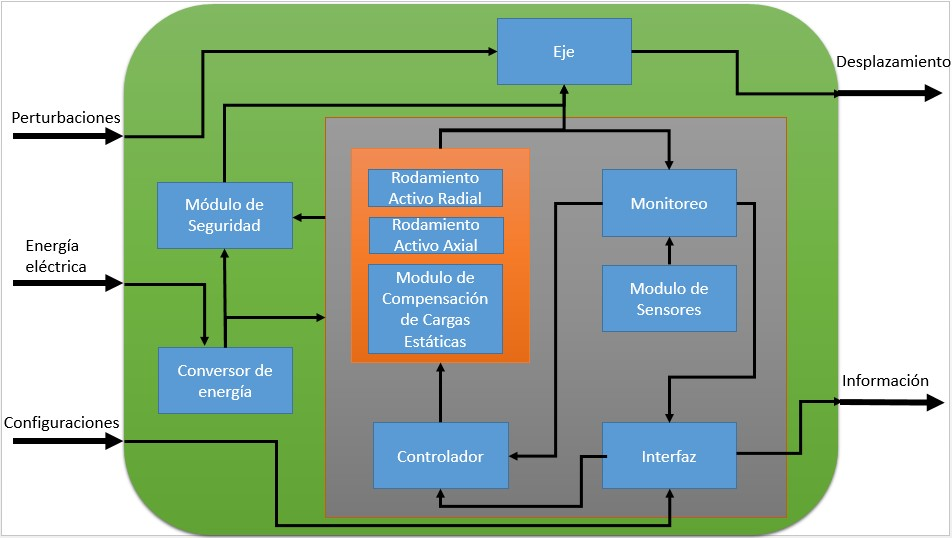
\includegraphics[width=\textwidth]{images/Capitulo_2/DiagramaFuncional}
	\caption{\textit{Diagrama Funcional.}}
	\label{fig:system:example1}
\end{figure}

\newpage

Del diagrama de �reas funcionales podemos reconocer que el sistema cuenta con 2 entradas que determinan el funcionamiento y el comportamiento del mismo: el suministro de energ�a el�ctrica y las perturbaciones que llegan al sistema. Este diagrama se divide en 3 secciones principales: la primera secci�n lo componen los m�dulos que generan los campos magn�ticos de levitaci�n, los cuales deben variar de acuerdo a lo que indique el controlador. Este se encuentra dominado por el monitoreo del m�dulo de sensores y la interfaz de usuario, la cual adem�s muestra informaci�n sobre la posici�n del rotor. 

La tercera secci�n incluye el convertidor de energ�a que alimenta todos los sistemas el�ctricos, incluyendo el m�dulo de seguridad, el cual se rige a trav�s de la informaci�n que provea el controlador, ya que este s�lo act�a con el corte del suministro el�ctrico o por alguna falla detectada por el controlador. 

\newpage

\section{An�lisis Morfol�gico}

La arquitectura del proyecto fue planteada con base en la investigaci�n te�rica sobre las caracter�sticas generales de los rodamientos magn�ticos y en la divisi�n por m�dulos funcionales que se hizo anteriormente, de manera que pudieran dise�arse de manera individual. 

Sin embargo, debido a que la cantidad de elementos mec�nicos u otros componentes a los que se les pudieran hacer modificaciones en cuanto a forma o disposici�n es muy poca, y considerando los principios b�sicos de operaci�n de cada uno de los m�dulos, la posibilidad de plantear una gran cantidad de variantes de dise�o es muy limitada. 

%\subsection{Rodamiento Magn�tico Activo Radial}

En el caso del rodamiento magn�tico activo para la carga radial se considero que estos utilizan un arreglo de electroim�nes opuestos para generar los campos magn�ticos de levitaci�n, y est�n dise�ados para soportar las cargas radiales que act�an sobre el rotor, manteni�ndolo centrado sobre el eje de rotaci�n. Considerando esto se plante� el siguiente concepto para la disposici�n de los electroim�nes:

\begin{figure}[htb]
\centering
	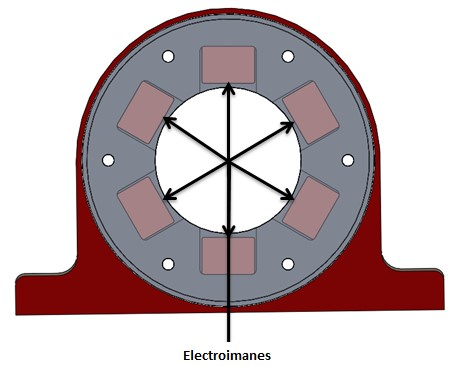
\includegraphics[scale=.65]{images/Capitulo_2/RMAR}
	\caption{\textit{Dise�o conceptual del rodamiento magn�tico activo radial.}}
	\label{fig:system:example1}
\end{figure}

Este es considerado el m�dulo central del rodamiento magn�tico h�brido, debido a que las dimensiones finales dependen principalmente del tama�o del arreglo de electroim�nes.  

%\subsection{Rodamiento Magn�tico Activo Axial}

\newpage

El siguiente m�dulo consiste en el rodamiento magn�tico activo axial el cual, como su nombre lo dice, est� dise�ado para soportar cargas axiales. Utilizan una pieza o collar de soporte constituido generalmente por un disco plano, s�lido, de material ferromagn�tico fijado al rotor. 

Los electroim�nes en forma de disco est�n situados en uno � a ambos lados del disco y sujetos a la carcasa o armaz�n del rodamiento. Ademas utilizan un sensor o arreglo de sensores que mide la posici�n del rotor en direcci�n axial. 

\begin{figure}[htb]
\centering
	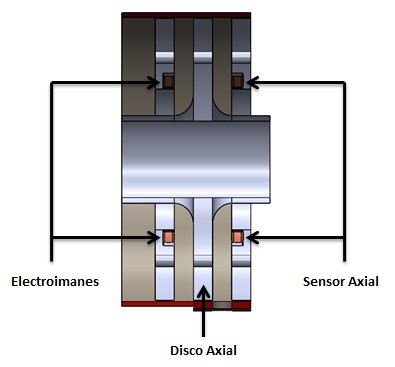
\includegraphics[scale=.65]{images/Capitulo_2/RMAA}
	\caption{\textit{Dise�o conceptual del rodamiento magn�tico activo axial.}}
	\label{fig:system:example1}
\end{figure}

%\subsection{M�dulo de Sensores}

Los rodamientos magn�ticos que funcionan por medio de electroim�nes utilizan sensores que miden la posici�n del eje y enviar estas se�ales de posici�n al controlador. El controlador utiliza esta informaci�n para modificar el campo electromagn�tico en el rodamiento, haciendo las correcciones necesarias para estabilizarlo.

Se plate� un arreglo de tres sensores dispuestos a 120� ya que por lo general este tipo de arreglo ofrece mejores mediciones.

\begin{figure}[htb]
\centering
	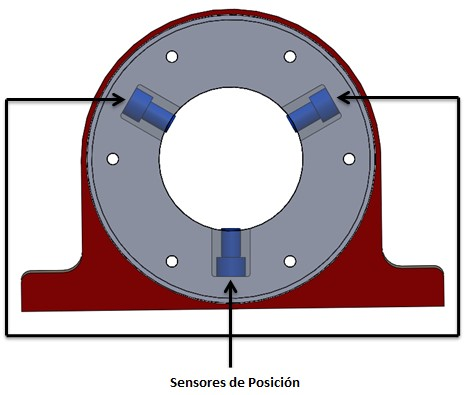
\includegraphics[scale=.65]{images/Capitulo_2/MS}
	\caption{\textit{Dise�o conceptual del arreglo de sensores para los desplazamientos radiales.}}
	\label{fig:system:example1}
\end{figure}

%\clearpage

%\subsection{M�dulo de Compensaci�n de Cargas Est�ticas}

\newpage

Como se ha mencionado en otras secciones, el proyecto consiste en un rodamiento magn�tico h�brido debido a que, ademas de utilizar electroim�nes como los rodamientos magn�ticos activos, utiliza un im�n permanente para generar un campo magn�tico base de levitaci�n siguiendo el principio de operaci�n de los rodamientos magn�ticos pasivos. Esto con el prop�sito de ayudar a disminuir el consumo de energ�a del rodamiento magn�tico radial.

Debido a que el campo magn�tico que genera el im�n permanente no puede ajustarse de la misma forma que los electroim�nes, este debe acoplarse a un mecanismo de desplazamiento que var�e la distancia entre el im�n permanente y el eje para ajustar el campo magn�tico. 

\begin{figure}[htb]
\centering
	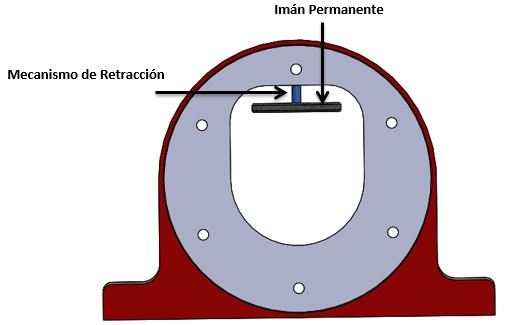
\includegraphics[scale=.70]{images/Capitulo_2/MCCE}
	\caption{\textit{Dise�o conceptual del m�dulo de compensaci�n para cargas est�ticas.}}
	\label{fig:system:example1}
\end{figure}

%\subsection{Collar�n de Levitaci�n}

Sin embargo, tanto el im�n permanente como los rodamientos magn�ticos activos necesitan que el rotor sea de un material ferromagn�tico para conseguir un estado de levitaci�n. 

Con el prop�sito de lograr la levitaci�n del rotor sin importar el material del que est� fabricado, se propone el uso de un collar�n de material ferromagn�tico que contenga al eje dentro del rodamiento. 

\begin{figure}[htb]
\centering
	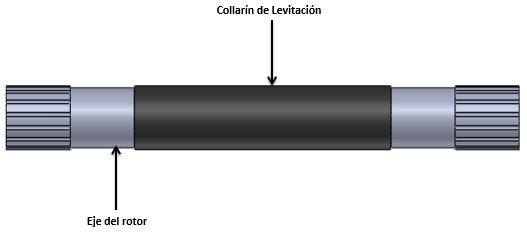
\includegraphics[scale=.80]{images/Capitulo_2/CL}
	\caption{\textit{Dise�o conceptual del collar�n de levitaci�n.}}
	\label{fig:system:example1}
\end{figure}

%\subsection{M�dulo de Seguridad}

Uno de los elementos m�s importantes con los que cuentan algunos de los rodamientos magn�ticos, sobretodo aquellos que trabajan con cargas muy grandes, es un mecanismo auxiliar que tenga como finalidad soportar el eje en caso de un corte en la energ�a o una falla en el controlador que pueda generar da�os a la m�quina. El rotor no debe de hacer contacto con el mecanismo auxiliar durante el funcionamiento normal de la m�quina.

\begin{figure}[h!]
\centering
	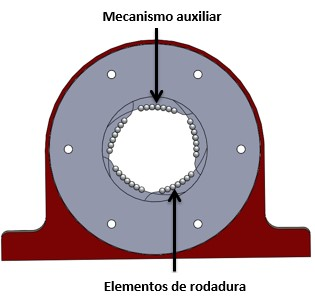
\includegraphics[scale=.80]{images/Capitulo_2/MSG}
	\caption{\textit{Dise�o conceptual del dispositivo auxiliar para el m�dulo de seguridad.}}
	\label{fig:system:example1}
\end{figure}

%\subsection{Rodamiento Magn�tico H�brido: Integraci�n de los M�dulos}

\newpage

Aunque cada uno de los m�dulos es dise�ado individualmente, est�n contemplados para funcionar de manera conjunta y ser ensamblados dentro del mismo armaz�n, procurando simplificar las operaciones de ensamble. La integraci�n de todos los m�dulos nos dar�a como resultado el Rodamiento Magn�tico H�brido. 

\begin{figure}[h!]
\centering
	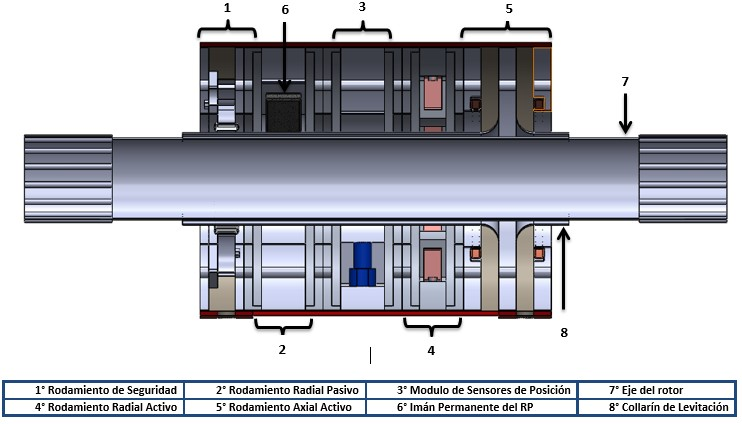
\includegraphics[width=\textwidth]{images/Capitulo_2/RMH}
	\caption{\textit{Dise�o Conceptual del Rodamiento Magn�tico H�brido.}}
	\label{fig:system:example1}
\end{figure}
%%%%%%%%%%%%%%%%%%%%%%%%%%%%%%%%%%%%%%%%%%%%%%%%%%%%%%%%%%%%%%%%%%%
%%%%%%%%%%%%%%%%%%%%%%%%%%%%%%%%%%%%%%%%%%%%%%%%%%%%%%%%%%%%%%%%%%%
\chapter{Dise\~no Detallado}
\section{Rodamiento magn�tico radial}

El Rodamiento Magn�tico Radial (RMR) consiste en un conjunto de electroimanes colocados en una circunferencia, de manera que sus campos magn�ticos puedan ejercer una fuerza arbitraria en su plano de acci�n. Para controlar la fuerza que cada electroim�n ejerce se tiene un circuito de accionamiento, que alimenta las bobinas del electroim�n con la corriente necesaria.

\begin{figure}[H]
    \centering
    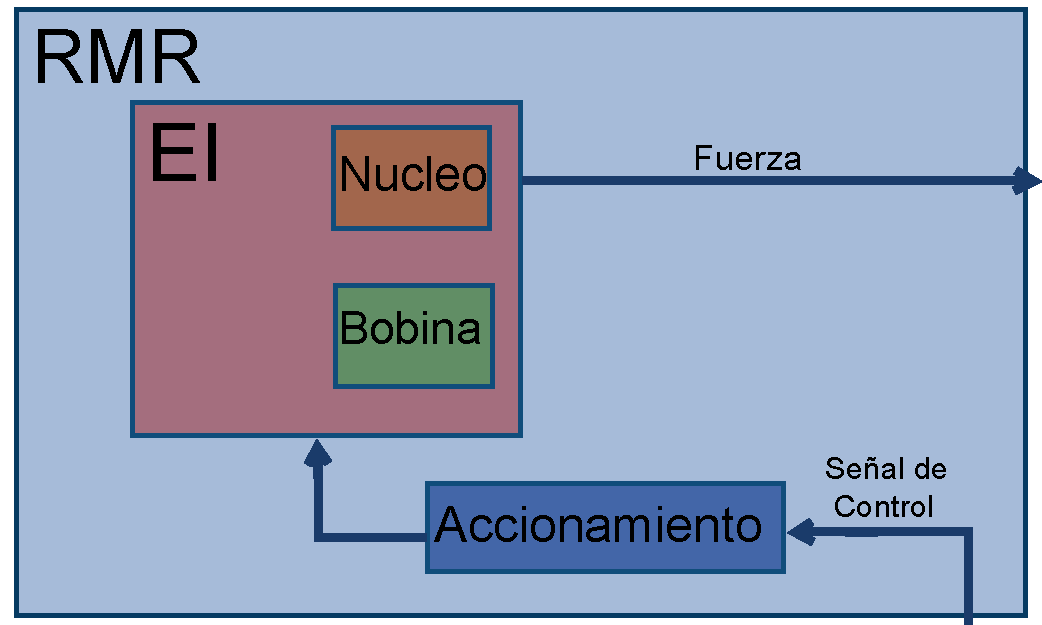
\includegraphics[width=0.625\textwidth]{images/Capitulo_3/diagrama_funcional_rmr}
    \caption{Diagrama funcional del rodamiento magn�tico radial.}
\end{figure}

\newpage

\subsection{N�mero de polos} \label{sec:numero-polos}

Antes de dise�ar los electroimanes es necesario determinar en n�mero de polos que conformar�n el EIR.
Suponiendo que tenemos $N$ polos, la distancia angular $\alpha$ entre ellos ser� de $360/N$ (fig. \ref{fig:rmr:diagrama-de-polos}). El EIR debe ser capaz de generar una fuerza arbitraria $F_r$ dentro del plano $YZ$. Teniendo en cuenta que los electroimanes s�lo son capaces de ejercer fuerzas de atracci�n sobre los materiales ferromagn�ticos. La fuerza $F_r$ deber� ser proporcionada �nicamente por las fuerzas de los electroimanes adyacentes $F_1$ y $F_2$ (fig. \ref{fig:rmr:diagrama-de-fuerzas}).  

\begin{figure}[H]
    \centering
    \begin{subfigure}[b]{0.4\textwidth}
        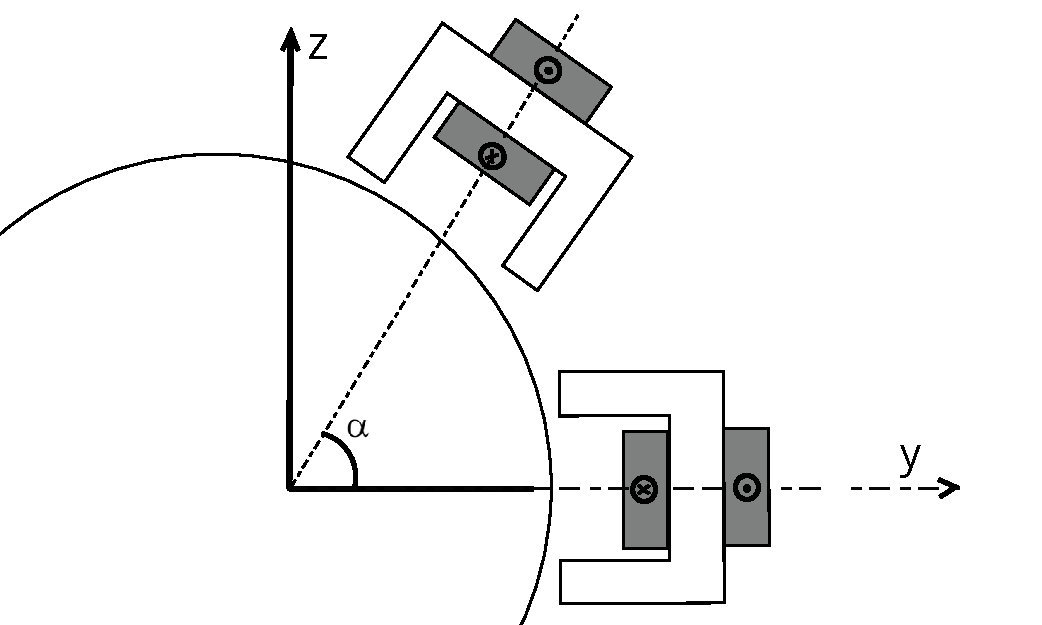
\includegraphics[width=\textwidth]{images/Capitulo_3/diagrama_polos}
        \caption{Posici�n de los polos.}
        \label{fig:rmr:diagrama-de-polos}
    \end{subfigure}
    ~ %add desired spacing between images, e. g. ~, \quad, \qquad, \hfill etc. 
      %(or a blank line to force the subfigure onto a new line)
    \begin{subfigure}[b]{0.4\textwidth}
        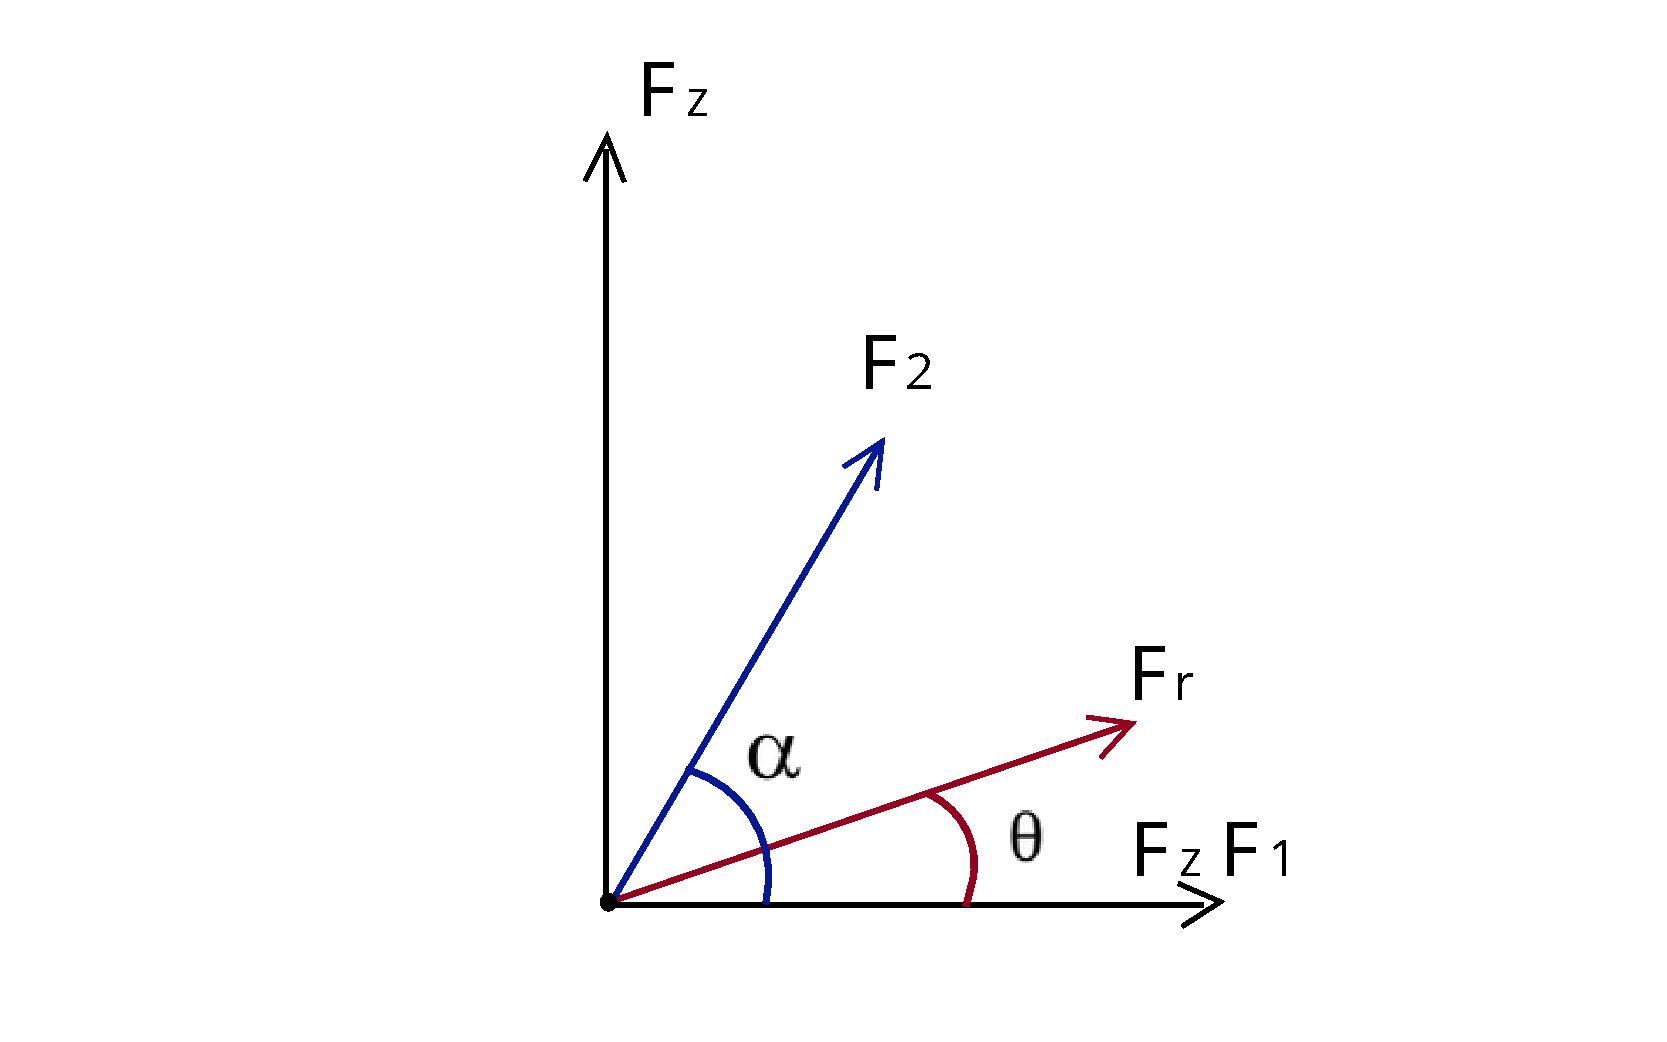
\includegraphics[width=\textwidth]{images/Capitulo_3/diagrama_fuerza_polos}
        \caption{Diagrama de Fuerzas.}
        \label{fig:rmr:diagrama-de-fuerzas}
    \end{subfigure}
    \caption{Polos del electroim�n radial.}
\end{figure}

Se define a $\theta$ como el �ngulo entre la fuerzas $F_r$ y $F_1$. Luego entonces, para una fuerza de magnitud $F_r$, las magnitudes de las fuerzas $F_1$ y $F_2$ ser�n: 
\begin{equation}
    F_1 = F_r (\frac{cos \theta - sin \theta}{tan \alpha})
\end{equation}
\begin{equation}
    F_2 = F_r (\frac{sin \theta}{sin \alpha} )
\end{equation}

Analizando los casos cr�ticos: 1) donde $F_r$ esta alineado con $F_1$ ($\theta = 0$), 2) donde $F_r$ esta orientado en medio de $F_1$ y $F_2$ ($\theta = \alpha/2)$ y 3) donde $F_r$ esta alineado con $F_2$ ($\theta = \alpha$); se vuelve clara la forma en la que el n�mero de polos afecta tanto la fuerza m�xima como la eficiencia del sistema.

Para los casos 1 y 3 toda la fuerza es ejercida por los electroimanes $E1$ y $E2$ respectivamente, con fuerzas de $F_1 = F_r, F_2 = 0$ para el caso 1, y $F_1 = 0, F_2 = F_r$ para el caso 3. Como lo indica la ecuaci�n:

\begin{equation}
P = (\frac{R F}{K_e} )
\end{equation}

Tendremos un consumo de magnitud $(\frac{R F_r}{K_e} )$. %, lo mismo sucede en el caso 3, 

En cambio en el caso 2 la fuerza tiene que ser proporcionada por F1 y F2 en partes iguales, y con una magnitud de:

\begin{equation}
F = F_1 = F_2 = (\frac{F_r sin (\frac{\alpha}{2}) }{sin \alpha} ) 
\end{equation}

Lo cual corresponde a una p�rdida de:

\begin{equation}
P = 2 (\frac{R F_r}{K_e} ) \label{eq:cosumo-electroiman-caso-especial}
\end{equation}

Para que el rodamiento axial pueda ejercer fuerzas en cualquier direcci�n del plano YZ es necesario un m�nimo de 3 polos. Sin embargo, incrementar el n�mero de polos reduce el consumo en las regiones intermedias (ecuaci�n \ref{eq:cosumo-electroiman-caso-especial}), ya que no estamos utilizando corriente para generar componentes de fuerza que terminar�n por cancelarse mutuamente.

En \cite{cite_s13_2017_matsuda2007_polos} se estudia de manera m�s detallada los efectos de variar el n�mero de polos en un RMR, se concluye que utilizar 6 polos minimiza el di�metro exterior para una capacidad dada.

\subsection{Electroim�n}

\subsubsection{Selecci\'on de Material} \label{sec:seleccion-somaloy}

En el caso de las aplicaciones de electroimanes, lo ideal es utilizar materiales con un alto punto de saturaci�n y permeabilidad relativa. El punto de saturaci�n limita la fuerza m�xima que puede ejercer un electroim�n [vease secci�n \ref{sec:diseno-elec}] y al tener una permeabilidad relativa alta podemos confiar que la mayor�a del flujo magn�tico circula dentro del n�cleo. 

Entre los materiales con estas caracter�sticas encontramos ferritas y aleaciones de hierro laminadas. Las ferritas poseen una alta permeabilidad pero tienen un punto de saturaci�n m�s bajo, mientras que las aleaciones de hierro poseen un punto de saturaci�n m�s alto y permeabilidad intermedia. Estos �ltimos al ser conductores presentan p�rdidas por corrientes par�sitas (corrientes de Foucault) que disminuye la eficiencia total del electroim�n.  

\begin{table}[H]
\centering
\begin{tabular}{|l|c|c|c|c|c|c|}
\hline
\multicolumn{1}{|c|}{\textbf{Fabricante}} & \textbf{Clave} & \textbf{Material Base} & \textbf{$\mu_i$} & \textbf{$B_s$ {[}mT{]}} & \textbf{$H_c$ {[}A/m{]}} & \textbf{$F_{max}$ {[}Hz{]}} \\ \hline
TDK {[}Anexo C{]} & PC90 & MnZn & 2200 & 540 & 13 & 300k \\ \hline
TDK {[}Anexo E{]} & N27 & MnZn & 2000 & 500 & 23 & 150k \\ \hline
Ferroxcube {[}Anexo F{]} & 3C98 & MnZn & 2500 & 530 & 12 & 400k \\ \hline
MMG \cite{cite_s22_2017_SoftFerrite} & F44 & MnZn & 2500 & 470 & 15 & 500k \\ \hline
NEC \cite{cite_s23_2017_FerriteCores} & BH3 & MnZn & 1800 & 540 & 15 & 400k \\ \hline
\end{tabular}
\caption{Propiedades de diferentes Ferritas MnZn.}
\end{table}

Como alternativa a los anteriores existen nuevos materiales como el Somaloy y Permalloy, estos son aleaciones de n�quel-hierro que gracias a su proceso de sinterizaci�n les permite alcanzar altos puntos de saturaci�n y permeabilidad relativa sin ser conductores. 

El Permalloy posee un punto de saturaci�n de 1.6 T y una permeabilidad relativa de 2500\cite{cite_s1_2017}, mientras que el Somaloy 3P posee un punto de saturaci�n de entre 1.42 y 1.63 y una permeabilidad relativa de 950 [v�ase anexo D]. 

A pesar de que el Permalloy posee mejores caracter�sticas, la empresa fabricante del Somaloy proporciona una documentaci�n m�s extensa en cuanto a las caracter�sticas de este como son: curva de saturaci�n a diferentes temperaturas, curvas de respuesta en frecuencia y caracterizaci�n de p�rdidas. Estos datos son de suma importancia al momento de realizar una simulaci�n y por eso se seleccion� el Somaloy como el material del n�cleo.      

\subsubsection{N�cleo ferromagn�tico}

De acuerdo a las especificaciones definidas en la secci�n \ref{sec:PDS} se estableci� una fuerza m�nima de:  

$$F_{min} = 50[N]$$

Al tratarse de un rodamiento con fines demostrativos, se propuso esa fuerza para que el resultado final ocupe el menor espacio posible.

El problema de seleccionar una distancia de operaci�n recae en que una distancia muy grande requiere una mayor inducci�n magn�tica para generar una fuerza determinada, mientras que con una distancia peque�a es m�s f�cil generar la misma fuerza con la desventaja de que se alcanza el punto de saturaci�n con mayor rapidez. Adem�s, si la distancia es muy peque�a hay poco espacio para estabilizarlo. 
 
En la literatura podemos identificar una distancia de operaci�n m�nima de $0.5 mm$ \citep{cite_s11_2017_Magnetic_Bearings_design} por lo que se opt� por trabajar con un rango de:

$$y_{max} = 0.75[mm]$$
$$y_{min} = 0.25[mm]$$

Teniendo en cuenta las caracter�sticas del material seleccionado y las condiciones de operaci�n descritas anteriormente se procede a utilizar las f�rmulas de la secci�n \ref{sec:diseno-elec}. 

$$A = 12 * 24 = 288[mm^2]$$

\subsubsection{C�lculo de la bobina} \label{sec:radial-calculo-bobina}

Como se explica en la secci�n \ref{sec:calc-conductores}, la relaci�n entre el n�mero de vueltas y la corriente depende del balance entre eficiencia y respuesta en frecuencia. Se opt� por utilizar una corriente de 2 A debido a la gran disponibilidad de componentes electr�nicos que operan a este valor de corriente, adem�s de ser un valor lo suficientemente alto como para que la inductancia no degrade la respuesta en frecuencia del electroim�n. 

$$I = 2[A]$$

De acuerdo a la tabla \ref{tabla:AWG-COBRE} para una corriente de 2 A corresponde a un calibre AWG de:

\begin{table}[H]
\centering
\begin{tabular}{|c|l|c|c|c|c|}
\hline 
AWG & Di\'ametro & Area\;($mm^2$) & Resistencia (ohms/km) & Corriente M�xima & Frecuencia M�xima\\ 
\hline 
18 & 1.023 & 0.823 & 20.94 & 2.3 & 17 $kHz$ \\
\hline  
\end{tabular} 
\caption{Especificaciones t�cnicas para el alambre de cobre esmaltado AWG 18.}
\label{tabla:awg-18}
\end{table}

Aplicando la siguiente f�rmula para determinar el n�mero de vueltas, obtenemos que:

\begin{equation}
N = \frac{NI_{max}}{I} = 314 [vueltas] \label{eq:vueltas-bobina}
\end{equation}

A trav�s de la f�rmula \ref{eq:area-bobina} y con las especificaciones del alambre esmaltado seleccionado, obtenemos la secci�n transversal de la bobina de:

$$A_b = 287.13 \; mm^2 \; \approx \; 288 \; mm^2$$

\begin{figure}[H]
    \centering
    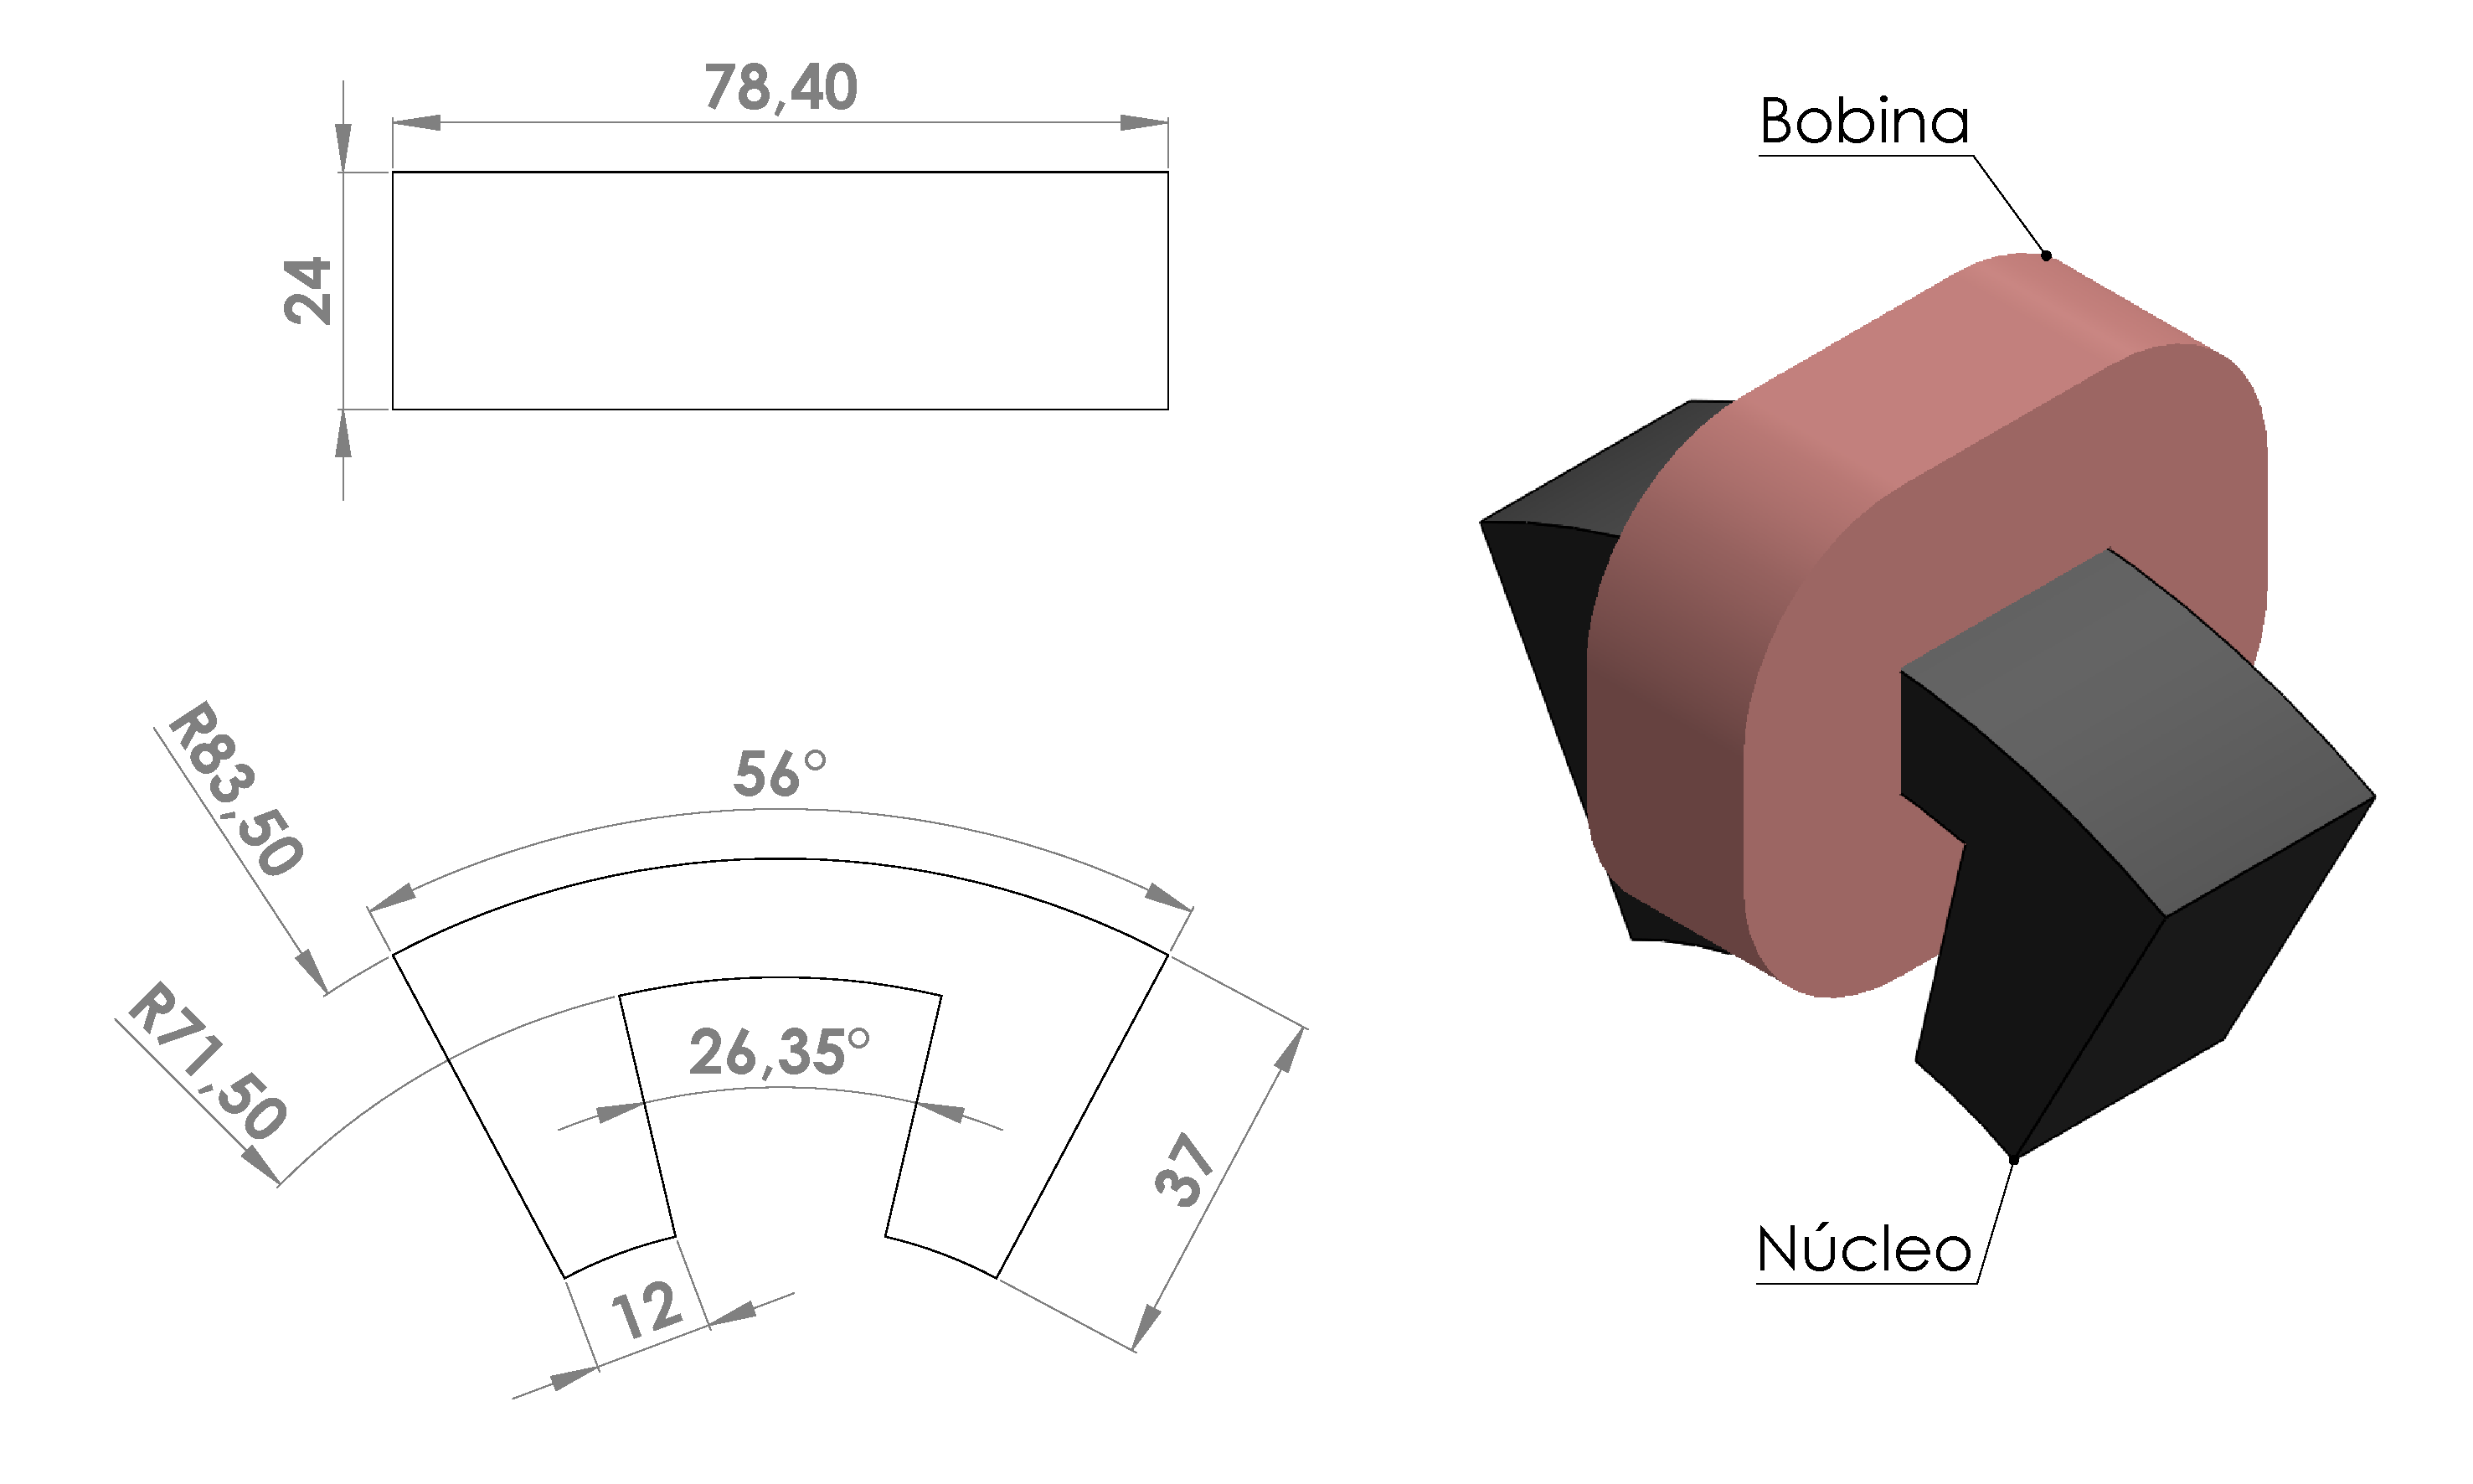
\includegraphics[width=0.8\textwidth]{images/Capitulo_3/electroiman_radial_final}
    \caption{Dimensiones del Electroim�n Radial.}
\end{figure}

\newpage

\subsection{Simulaci�n FEM} \label{sec:simulacion-fem-electroiman}

Con el fin de validar los c�lculos y comprobar que el n�cleo no alcance su punto de saturaci�n, se realiz� una simulaci�n de elemento finito con ayuda del software FEMM donde se obtuvieron los siguientes resultados:
\begin{figure}[H]
    \centering
    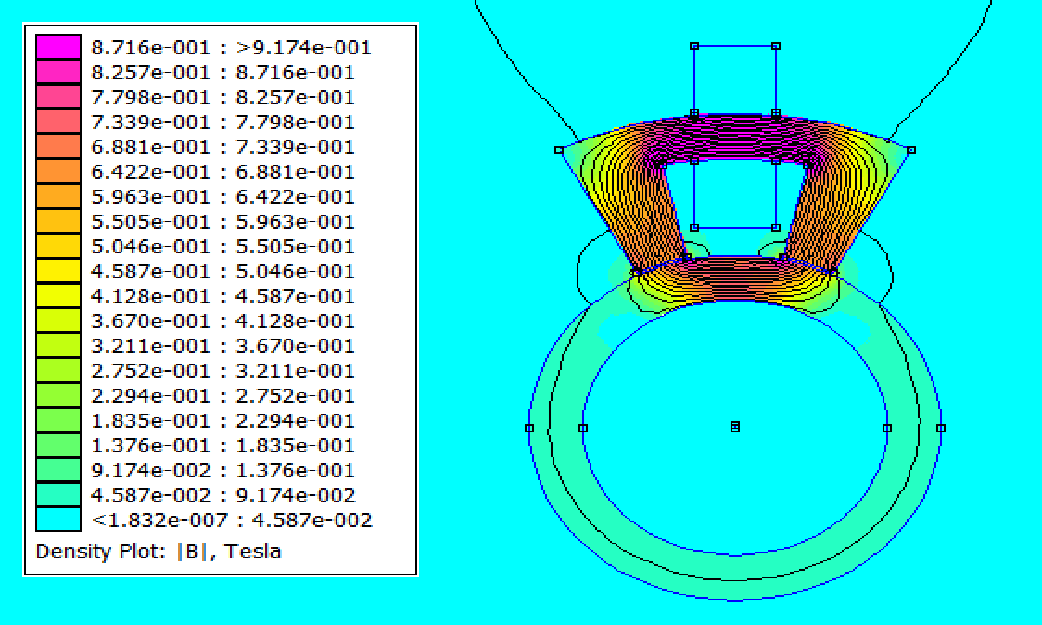
\includegraphics[width=0.8\textwidth]{images/Capitulo_3/simulacion_radial}
    \caption{Simulaci�n del electroim�n radial en FEMM.}
    \label{fig:simulacion-femm-radial}
\end{figure}
En la figura \ref{fig:simulacion-femm-radial} se puede observar que el valor m�ximo de inducci�n magn�tica es de $0.917 T$ lo cu�l est� por debajo del punto de saturaci�n del material.

Existe una diferencia entre el modelo ideal y la simulaci�n. Esta diferencia se debe a los efectos de la reluctancia del n�cleo. Un modelo que incluya la reluctancia del n�cleo se acerca m�s al modelo real tal y como se muestra en la figura \ref{fig:curva-fuerza-rmr}.
\begin{figure}[H]
    \centering
    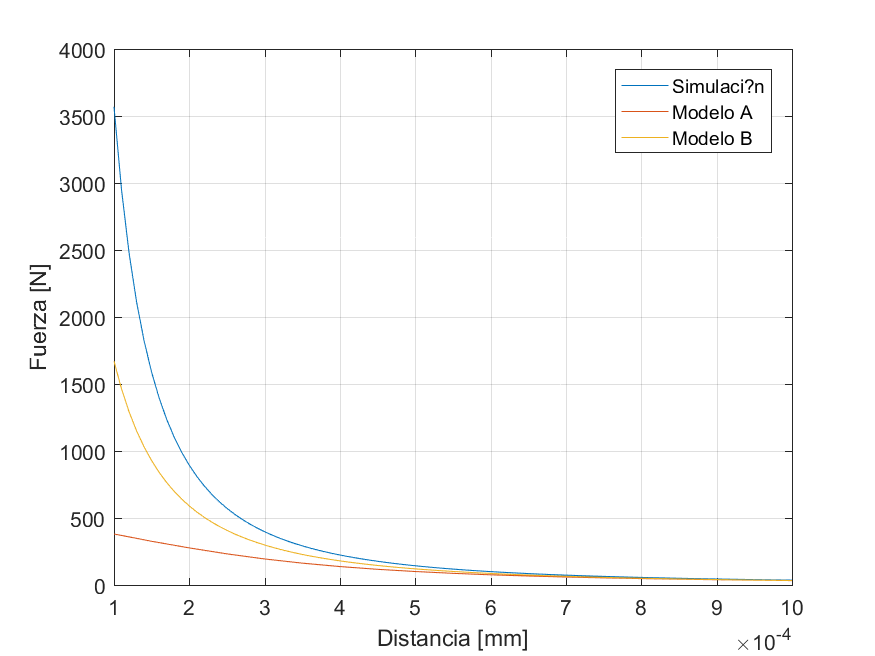
\includegraphics[width=0.8\textwidth]{images/Capitulo_3/simulacion_vs_modelo_radial}
    \caption{Curva Fuerza - Distancia del RMR.}
    \label{fig:curva-fuerza-rmr}
\end{figure}

\subsection{Electr�nica de accionamiento}

Ahora que conocemos las caracter�sticas de los electroimanes, es necesario un circuito para controlar la corriente que circula por la bobinas. Para este punto ya conocemos las caracter�sticas el�ctricas de las bobinas como la inductancia y la resistencia. Estos datos nos servir�n mas adelante para calcular una circuiteria con un bajo �ndice de p�rdidas. 

\begin{figure}[H]
    \centering
    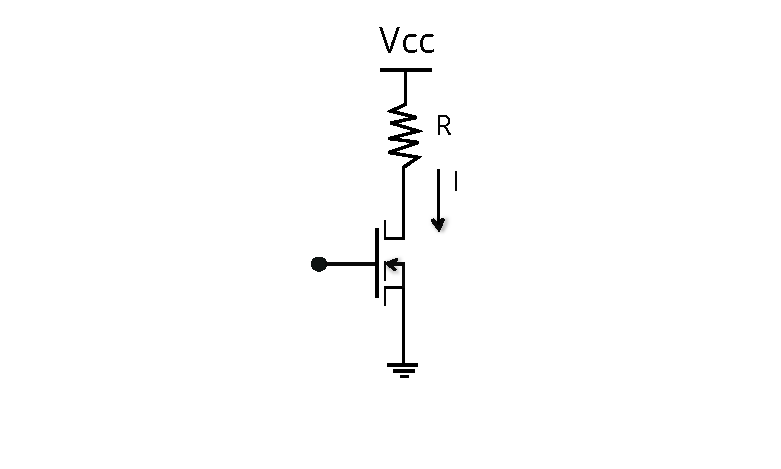
\includegraphics[width=0.5\textwidth]{images/Capitulo_3/MOSFET_1}
    \caption{Amplificador lineal.}
    \label{fig:amplificador-lineal}
\end{figure}

Un amplificador que opera en modo lineal, como el de la figura \ref{fig:amplificador-lineal}, opera de la siguiente manera: supongamos que tenemos que hacer pasar una corriente de 1 ampere a trav�s de una carga de 10 Ohms, para que exista 1 ampere se necesitan 10 volts. Si nuestra fuente es de 20 volts esto implica que el transistor debe de absorber los 10 volts restantes. Esto implica disipar 10 W de potencia en forma de calor. Entonces es evidente la baja eficiencia que resulta operar de este modo.

En cambio si operamos en el modo de saturaci�n tendr�amos en las terminales del transistor 0 volts y 20 amperes, mientras que en la zona de corte tendriamos 20 volts y 0 amperes. Ambas situaciones corresponden a una potencia disipada de 0 W en el transistor. En otras palabras, la disipaci�n de energ�a en forma de calor es m�nima. 

Para regular la corriente que circula conmutamos de un estado a otro de manera que el promedio de la corriente sea la corriente deseada.

De manera pragm�tica, esta conmutaci�n se realiza mediante transistores MOSFET debido a su baja resistencia en encendido Ron. El MOSFET es un dispositivo que controla la corriente a trav�s del voltaje aplicado en sus terminales, donde la relaci�n entre estas se encuentra determinada por:

\begin{equation}
I_d = G(V_g - V_{th})^2
\end{equation}

Donde $V_{th}$, conocido como voltaje de treshhold, es el voltaje m�nimo para activar el transistor. Una vez el voltaje de compuerta $Vg$ llega sobrepasa el valor $V{sat}$ el transistor no deja incrementar m�s la corriente y simplemente se comporta como una resistencia de valor $R_{on}$. A este modo de operaci�n se le conoce como saturaci�n.

Cuando se trata de conmutar una carga inductiva se generan picos de voltaje, pues la corriente que circula por un inductor no puede cambiar de manera instant�nea o discontinua. Es por eso que se necesita de un diodo para proveer un camino por el que la corriente logre recircular y disminuir de manera controlada.

\begin{figure}[H]
    \centering
    \begin{subfigure}[b]{0.4\textwidth}
        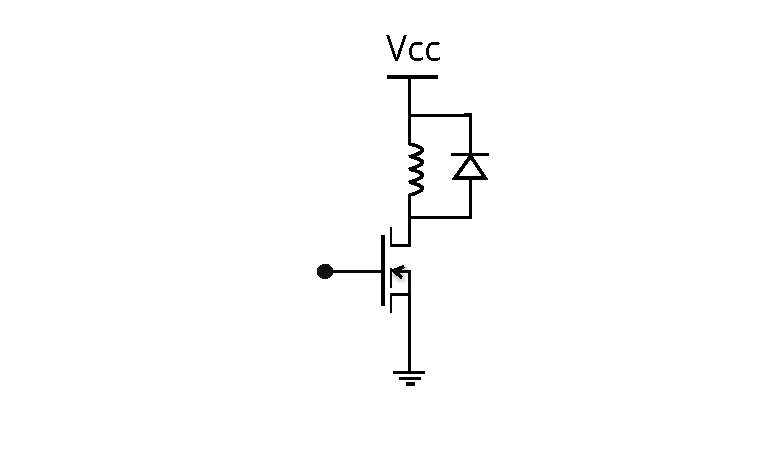
\includegraphics[width=\textwidth]{images/Capitulo_3/MOSFET_2}
        \caption{Circuito con diodo de recirculaci�n.}
        \label{fig:circuito-recirculacion}
    \end{subfigure}
    ~ %add desired spacing between images, e. g. ~, \quad, \qquad, \hfill etc. 
      %(or a blank line to force the subfigure onto a new line)
    \begin{subfigure}[b]{0.4\textwidth}
        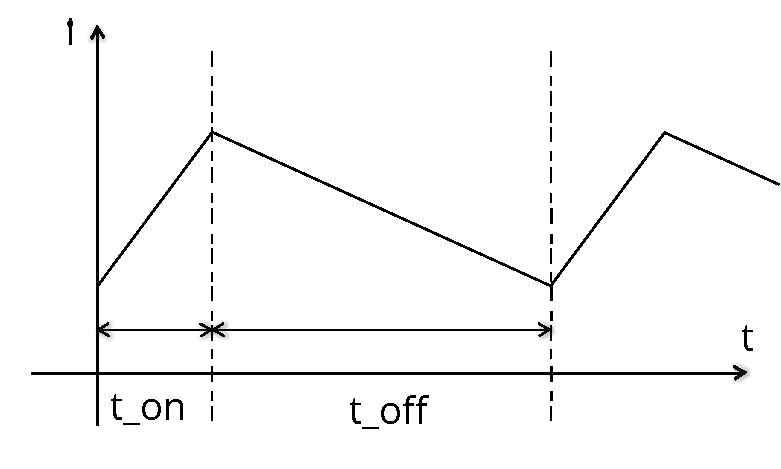
\includegraphics[width=\textwidth]{images/Capitulo_3/Grafica_Accionamiento_simple}
        \caption{Carga y descarga del inductor.}
        \label{fig:carga-descarga-inductor-simple}
    \end{subfigure}
\end{figure}

La raz�n de cambio en la corriente en un inductor depende del voltaje aplicado en sus terminales. En el circuito \ref{fig:circuito-recirculacion}, cuando el transistor est� activado el voltaje en las terminales es $V_{cc} \approx 20$, y cuando est� desactivado (y la corriente circula por el diodo) el voltaje en las terminales es el voltaje de diodo $V_d \approx 0.5$. Entonces los valores de carga y descarga del inductor ser�n de:

\begin{equation}
\frac{di}{dt}_{on} = \frac{V_{cc}}{L}
\end{equation}

\begin{equation}
\frac{di}{dt}_{off} = \frac{-2V_{cc}}{L}
\end{equation}

El problema es que el incremento y decremento de la corriente act�an de forma asim�trica (fig. \ref{fig:carga-descarga-inductor-simple}), entonces para obtener cargas y descargas sim�tricas ser� necesario aplicar un voltaje de $-V_{cc}$ durante el ciclo de descarga. Para eso es necesaria una configuraci�n como la mostrada en la figura \ref{fig:puente-h}.

\begin{figure}[H]
    \centering
    \begin{subfigure}[b]{0.4\textwidth}
        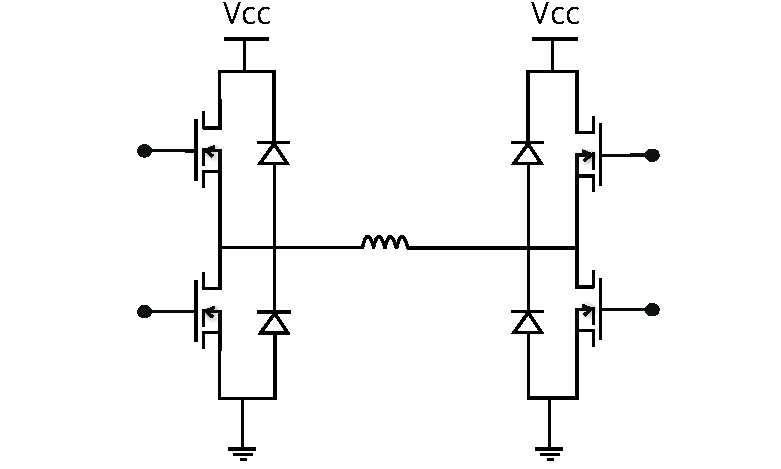
\includegraphics[width=\textwidth]{images/Capitulo_3/Puente_H}
        \caption{Circuito de Puente H.}
        \label{fig:puente-h}
    \end{subfigure}
    ~ %add desired spacing between images, e. g. ~, \quad, \qquad, \hfill etc. 
      %(or a blank line to force the subfigure onto a new line)
    \begin{subfigure}[b]{0.4\textwidth}
        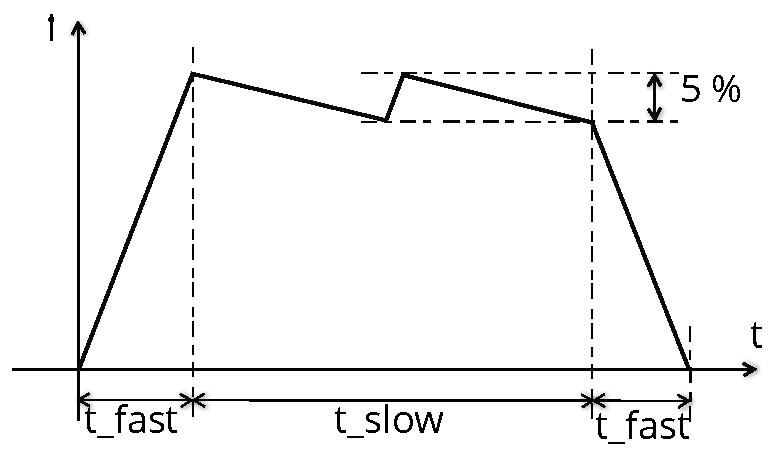
\includegraphics[width=\textwidth]{images/Capitulo_3/Grafica_accionamiento_avanzado}
        \caption{Carga y descarga r�pida.}
        \label{fig:carga-descarga-rapida}
    \end{subfigure}
\end{figure}

Esta configuraci�n es com�nmente conocida como puente "H" e implica varios detalles para su implementaci�n, el primero de estos es la activaci�n de los transistores. Como ya se ha mencionado, para operar de la manera m�s eficiente es necesario llevar los transistores a su punto de saturaci�n, en la mayor�a de los transistores de potencia el voltaje de compuerta en saturaci�n $V_{sat}$ oscila entre los 10 y 15 volts, y dado que la mayor�a de los circuitos de procesamiento operan entre los 5 y 1.8 volts, es necesario de un circuito complementario para elevar los niveles de voltaje. No hacer esto causar�a la polarizaci�n de los transistores en la zona lineal, lo que resultar�a en el calentamiento de estos y una operaci�n con baja eficiencia. 

Otro problema consiste en polarizar los transistores de la figura \ref{fig:puente-h}, ya que para su correcta activaci�n es necesario un voltaje de compuerta de hasta $V_{cc} + V{sat}$. 

Ambos problemas son solucionados mediante el uso de un circuito conocido como Gate Driver, donde se usa un arreglo de transistores, diodos y capacitores para proveer los voltajes correctos en las compuertas de los transistores sin necesidad de una fuente separada.

Suponiendo que queremos mantener constante la corriente del inductor podemos desactivar todos los transistores dej�ndolos recircular por los diodos. Cuando la corriente recircula por los diodos, �sta disminuye en una raz�n de:

\begin{equation}
\frac{di}{dt} = \frac{-2V_d}{L}
\end{equation}

Como la resistencia de los transistores Ron es baja, si activamos los transistores 1 y 2 recirculando la corriente por estos la tasa de cambio ser�:

\begin{equation}
\frac{di}{dt} = \frac{R i}{L}
\end{equation}

A este modo de operaci�n se le conoce como rectificaci�n s�ncrona. Esto no se puede realizar con transistores bipolares, pero si con transistores MOSFET. 

Podemos definir ahora dos estados de operaci�n del puente H, un modo de accionamiento, donde se incrementa o decrementa la corriente en la bobina ($t_{fast}$ de la figura \ref{fig:carga-descarga-rapida}), y un modo de recirculaci�n, donde la corriente se mantiene a un nivel casi constante, y donde solo est�n presentes la p�rdidas resistivas causadas por $R_{ESR}$ y $R_{on}$ ($t_{slow}$ de la figura \ref{fig:carga-descarga-rapida}).

Estos modos de operaci�n puede implementarse usando el circuto de la figura \ref{fig:circuito-control-corriente}, donde el arreglo de comparadores y flip flops permite controlar la corriente.

\begin{figure}[H]
    \centering
    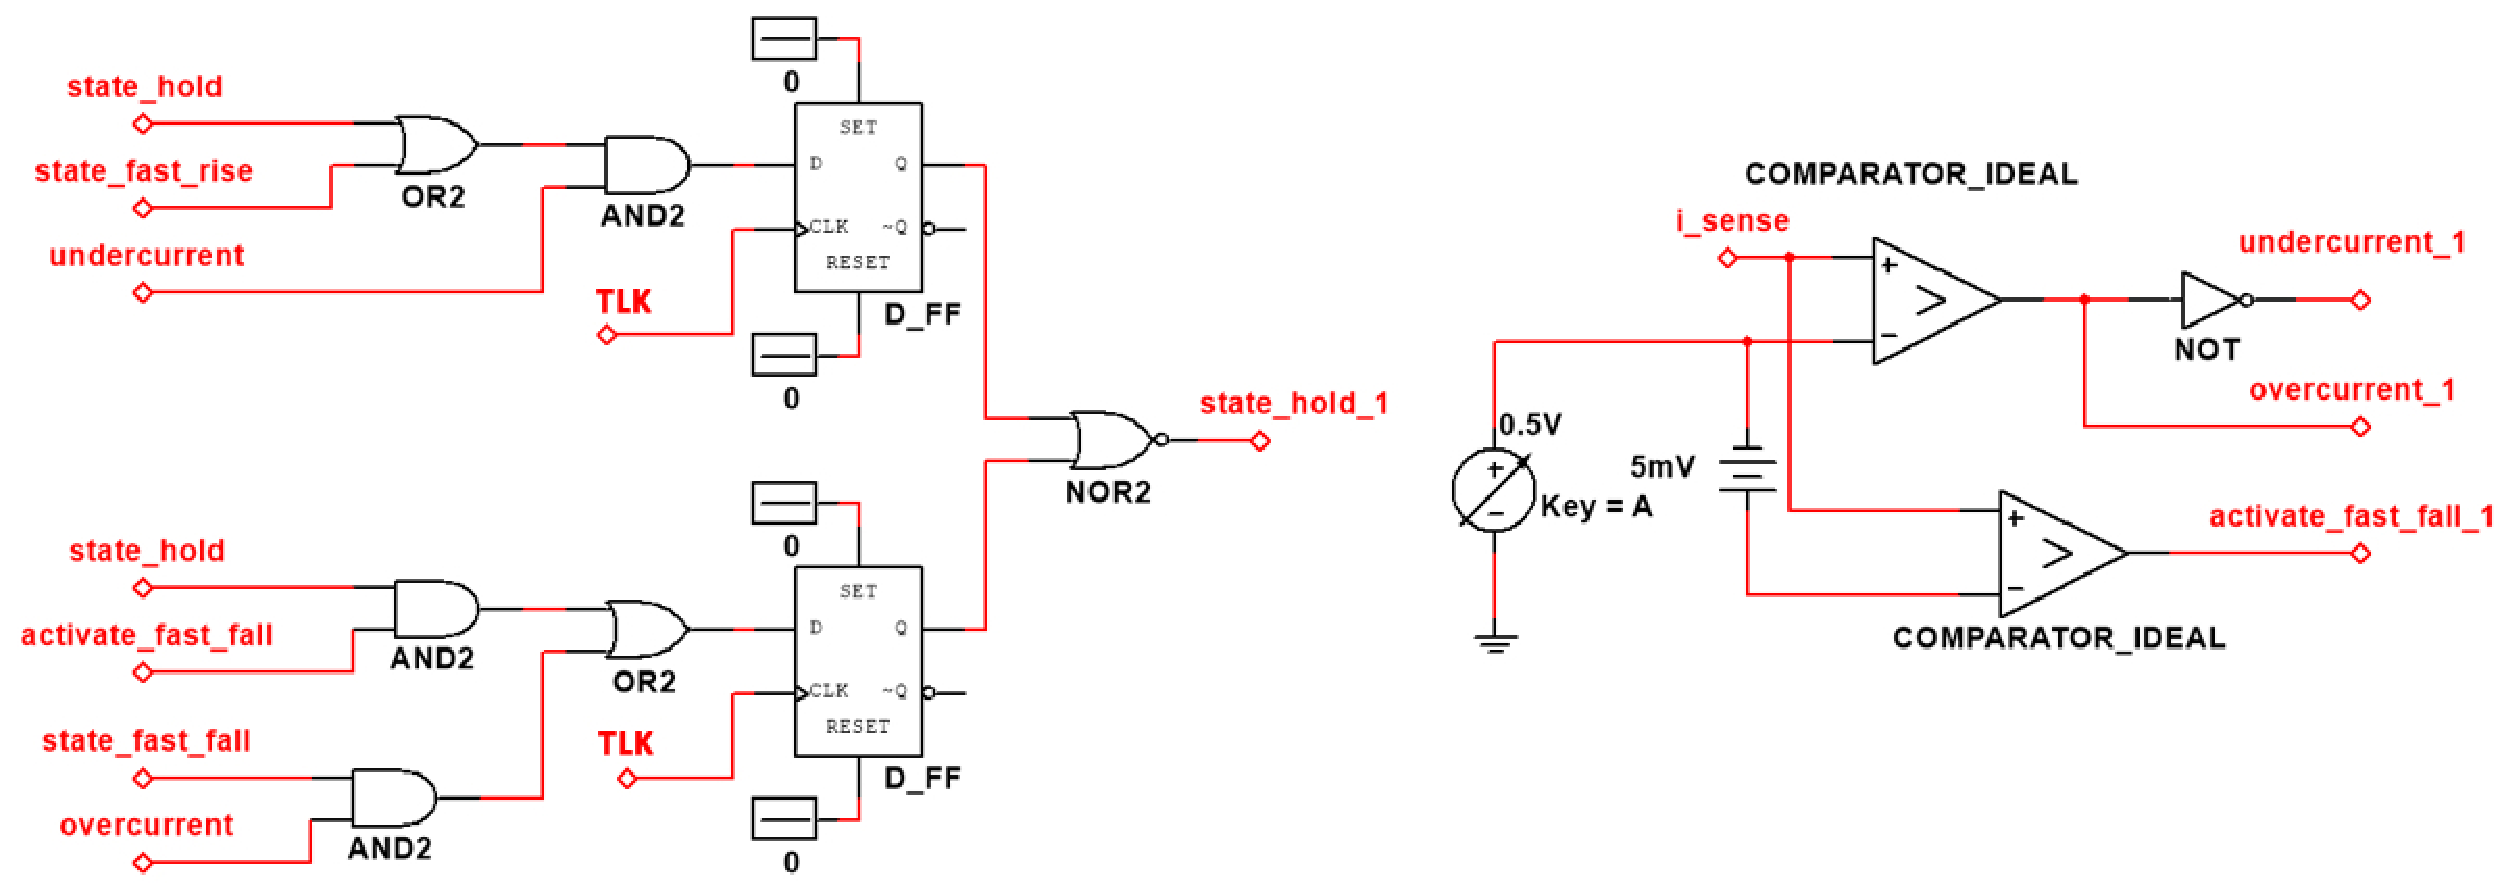
\includegraphics[width=\textwidth]{images/Capitulo_3/circuito-control-corriente}
    \caption{Circuito de control de la corriente.}
    \label{fig:circuito-control-corriente}
\end{figure}

Como ya se ha mencionado, la raz�n de cambio en la corriente de un inductor est� limitada por su inductancia. Esto implica que si tratamos de generar  una se�al senoidal, la frecuencia m�xima $F_{max}$ que podr�amos producir sin distorsionarla ser�a:

\begin{equation}
\frac{di}{dt}_{max} = 2 \pi f_{max} A = \frac{L}{V} 
\label{eq:respuesta-frecuencia-accionamiento-1}
\end{equation}

Donde $V$ es el voltaje de alimentaci�n del circuito. Si despejamos la frecuencia m�xima tenemos:

\begin{equation}
f_{max} = \frac{L}{2 \pi V A} 
\label{eq:respuesta-frecuencia-accionamiento-2}
\end{equation} 

Podemos ver que la frecuencia m�xima de la se�al de salida depende de la amplitud de la misma. Esta condici�n  conocida como "slew rate limiting" es un fen�meno com�n en los amplificadores y basta con conocer los limites de operaci�n del dispositivo para evitar esta situaci�n.

\begin{figure}[H]
    \centering
    \begin{subfigure}[b]{0.4\textwidth}
        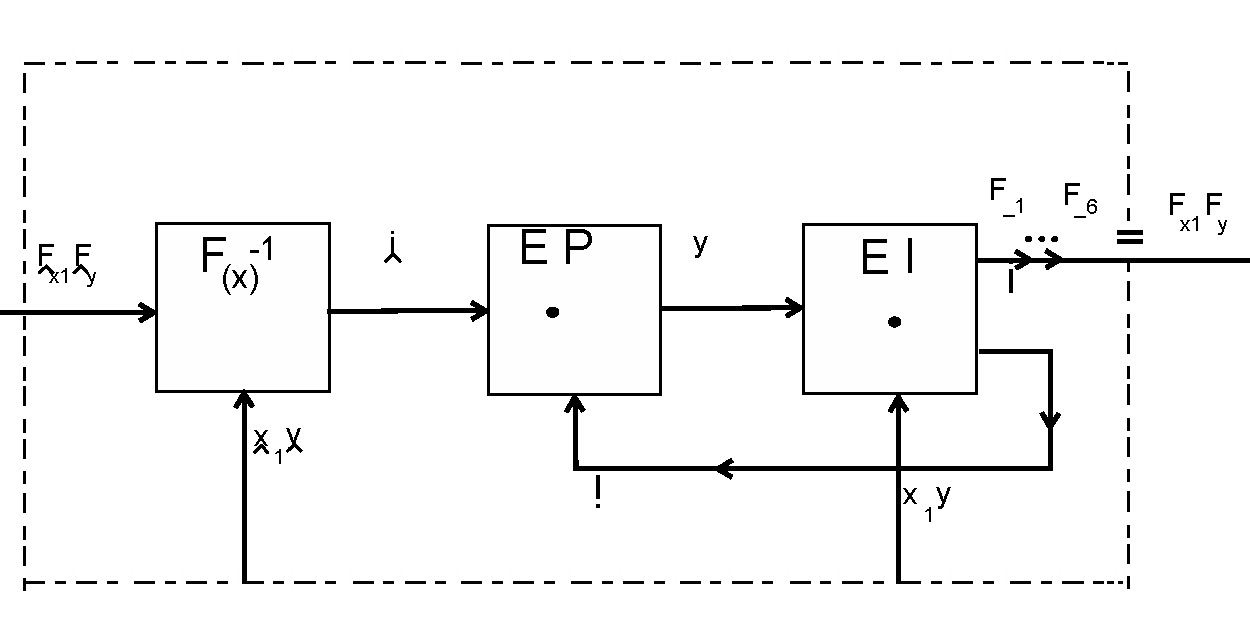
\includegraphics[width=\textwidth]{images/Capitulo_2/fb_linearization}
        \caption{Esquema de retroalimentacion.}
    \end{subfigure}
    ~ %add desired spacing between images, e. g. ~, \quad, \qquad, \hfill etc. 
      %(or a blank line to force the subfigure onto a new line)
    \begin{subfigure}[b]{0.4\textwidth}
        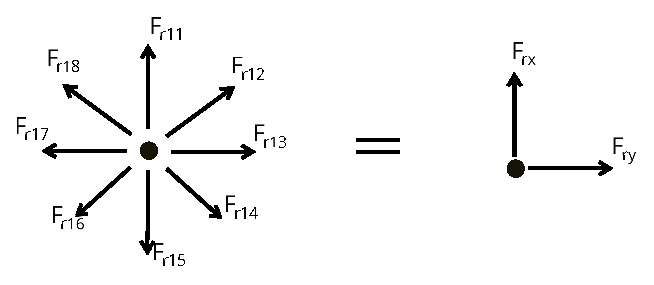
\includegraphics[width=\textwidth]{images/Capitulo_2/ferzas_radial}
        \caption{Equivalencia de fuerzas.}
    \end{subfigure}
    \caption{Linearizaci�n de electroimanes.}
\end{figure}

En caso de operar mas all� de los limites frecuencia-amplitud, se presentar� una atenuaci�n de magnitud:

\begin{equation}
A = \frac{L}{2 \pi V f} 
\end{equation} 

Esta atenuaci�n coincide con la de un filtro pasabajas de primer orden, con frecuencia de corte $f_{max}$ y una ca�da de $20dB$ por d�cada. Para los electroimanes presentados en \ref{sec:radial-calculo-bobina} esta respuesta corresponde a las gr�ficas de la figura \ref{fig:respuesta-frecuencia-electroiman}. 

\begin{figure}[H]
    \centering
    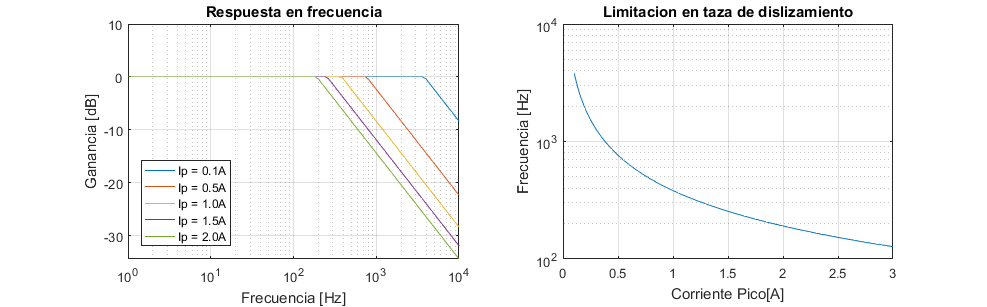
\includegraphics[width=\textwidth]{images/Capitulo_3/respuesta_dinamica_cp}
    \caption{Respuesta en frecuencia del circuito de accionamiento.}
    \label{fig:respuesta-frecuencia-electroiman}
\end{figure}

Una vez ensamblado el conjunto de electroimanes resulta en el modelo de la figura \ref{fig:Modelo-3D-RMR}.

\begin{figure}[H]
    \centering
    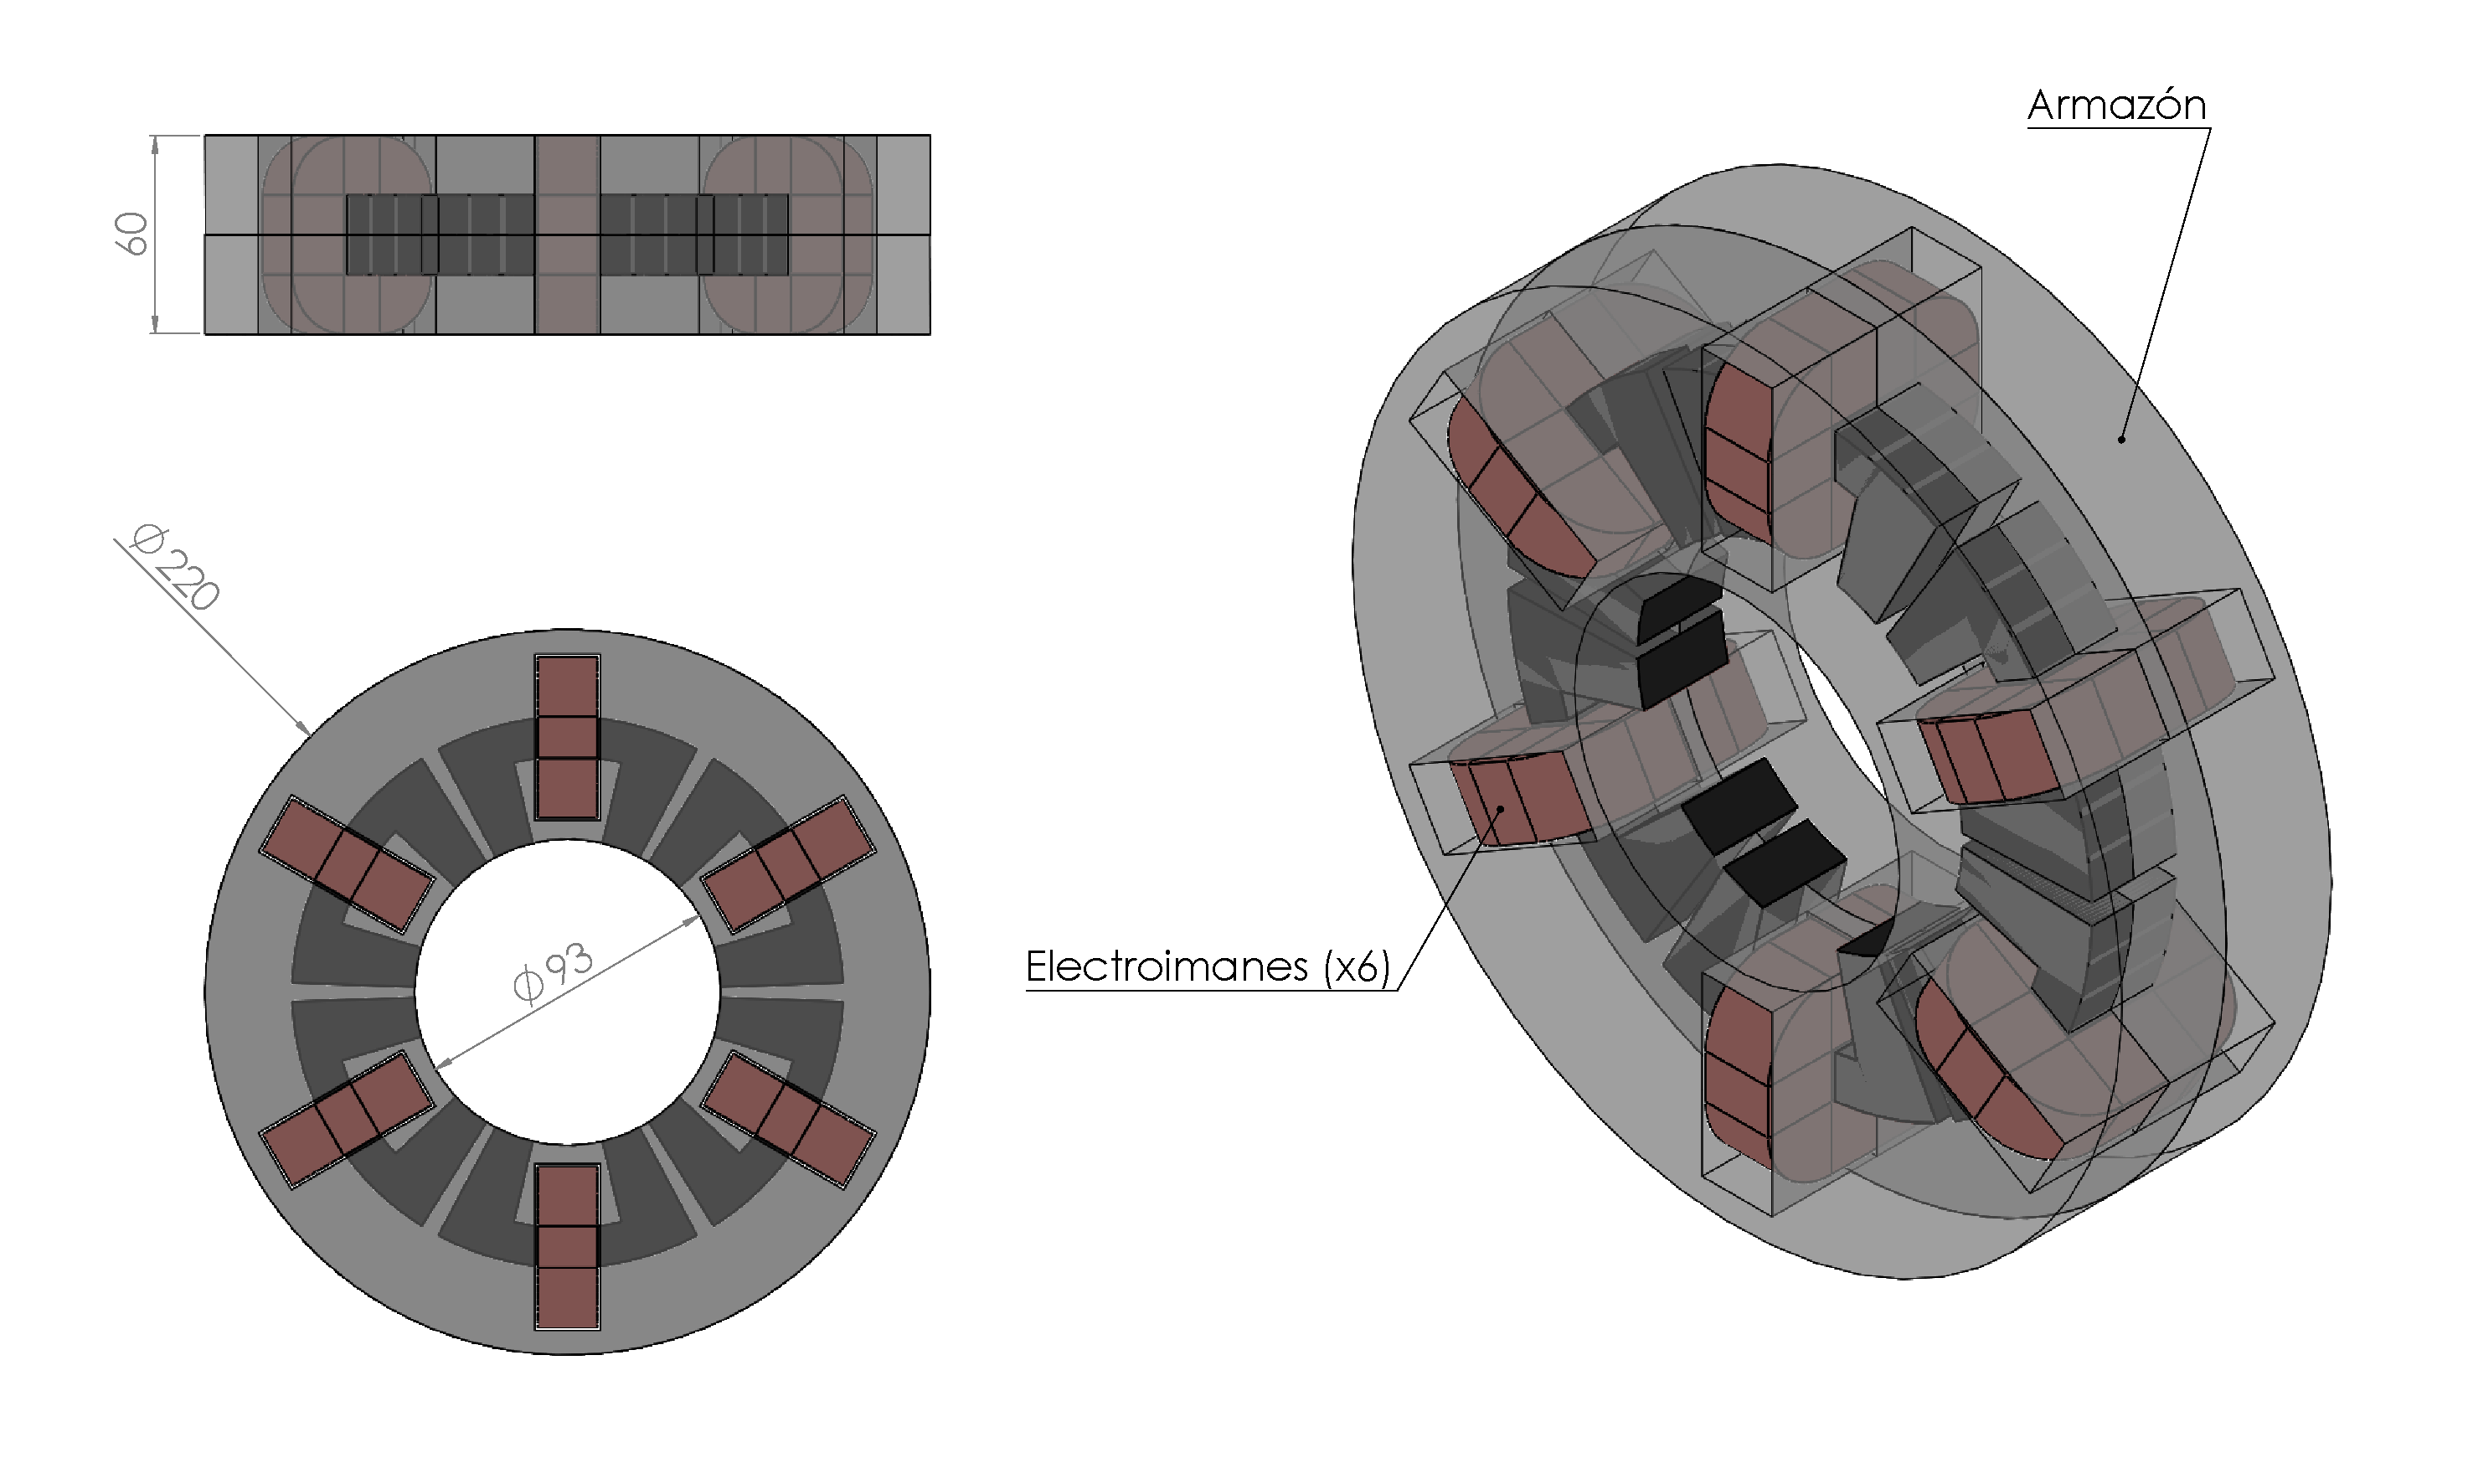
\includegraphics[width=0.8\textwidth]{images/Capitulo_3/EIR_assembly}
    \caption{Modelo final del Rodamiento Magn�tico Radial (RMR).}
    \label{fig:Modelo-3D-RMR}
\end{figure}

\newpage

\section{Rodamiento magn�tico axial}

El Rodamiento Magn�tico Axial (RMA) sirve para ejercer fuerzas de atracci�n alineadas con el eje de rotaci�n del rodamiento. Consiste en un par de electroimanes axisim�tricos ubicados en los extremos del eje y una electr�nica de accionamiento para activar dichos electroimanes. Estos tienen que actuar en pares para ejercer fuerzas en ambas direcciones del eje. 

\begin{figure}[h]
    \centering
    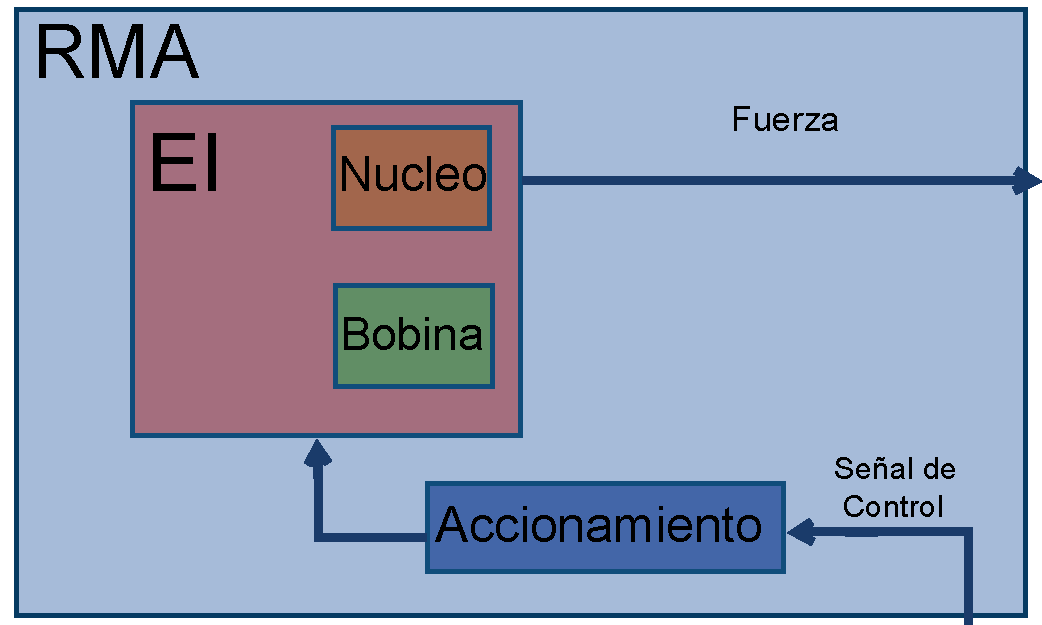
\includegraphics[width=0.625\textwidth]{images/Capitulo_3/diagrama_funcional_rma}
    \caption{Rodamiento magn�tico axial.}
\end{figure}

\newpage

\subsection{Electroim�n}

\subsubsection{N�cleo ferromagn�tico}

Como se realiz� en la secci�n \ref{sec:seleccion-somaloy} se selecciona el material Somaloy 3P [hoja de datos en anexo D] para formar el n�cleo del electroim�n, este material tiene unas caracter�sticas de: 

\begin{itemize}
\item Punto de saturaci�n: $1.42 - 1.63 T$
\item Permeabilidad relativa: $\mu_r = 950$
\end{itemize}

Debido a que las cargas principales se encuentran en el plano de acci�n del RMR, no es necesario que el RMA posea la misma capacidad de carga. Entonces, con la finalidad de reducir el espacio que ocupa el RMA, se seleccion� una fuerza de $F_{min} = 10 N$. 

Como se requiere aplicar una menor fuerza es posible utilizar un rango de operaci�n m�s grande. De esta manera se estableci� un rango de:

$$y_{max} = 2[mm]$$
$$y_{min} = 1.0[mm]$$

Siguiendo el procedimiento desarrollado en la secci�n \ref{sec:diseno-elec}, y con los par�metros establecidos anteriormente, se lleg� a una secci�n transversal de:

$$A = \frac{36 \pi}{4} = 1017[mm^2]$$

\subsubsection{C�lculo de la bobina}

Con el fin de usar la misma electr�nica de accionamiento para controlar el electroim�n axial, se opt� por usar el mismo valor de corriente en las bobinas de $I = 2 A$. 

Retomando la secci�n \ref{sec:radial-calculo-bobina}, para una corriente de $2 A$ corresponde un calibre AWG $18$ [ver tabla \ref{tabla:awg-18}.

Para el c�lculo del n�mero de vueltas se utiliza la ecuaci�n \ref{eq:vueltas-bobina} resultando en $162$ vueltas.

Con los par�metros anteriores y con la f�rmula \ref{eq:area-bobina} se determina un �rea m�nima de: $148.14 \; mm^2 \; \approx \; 148 \; mm^2$. 

\begin{figure}[h]
    \centering
    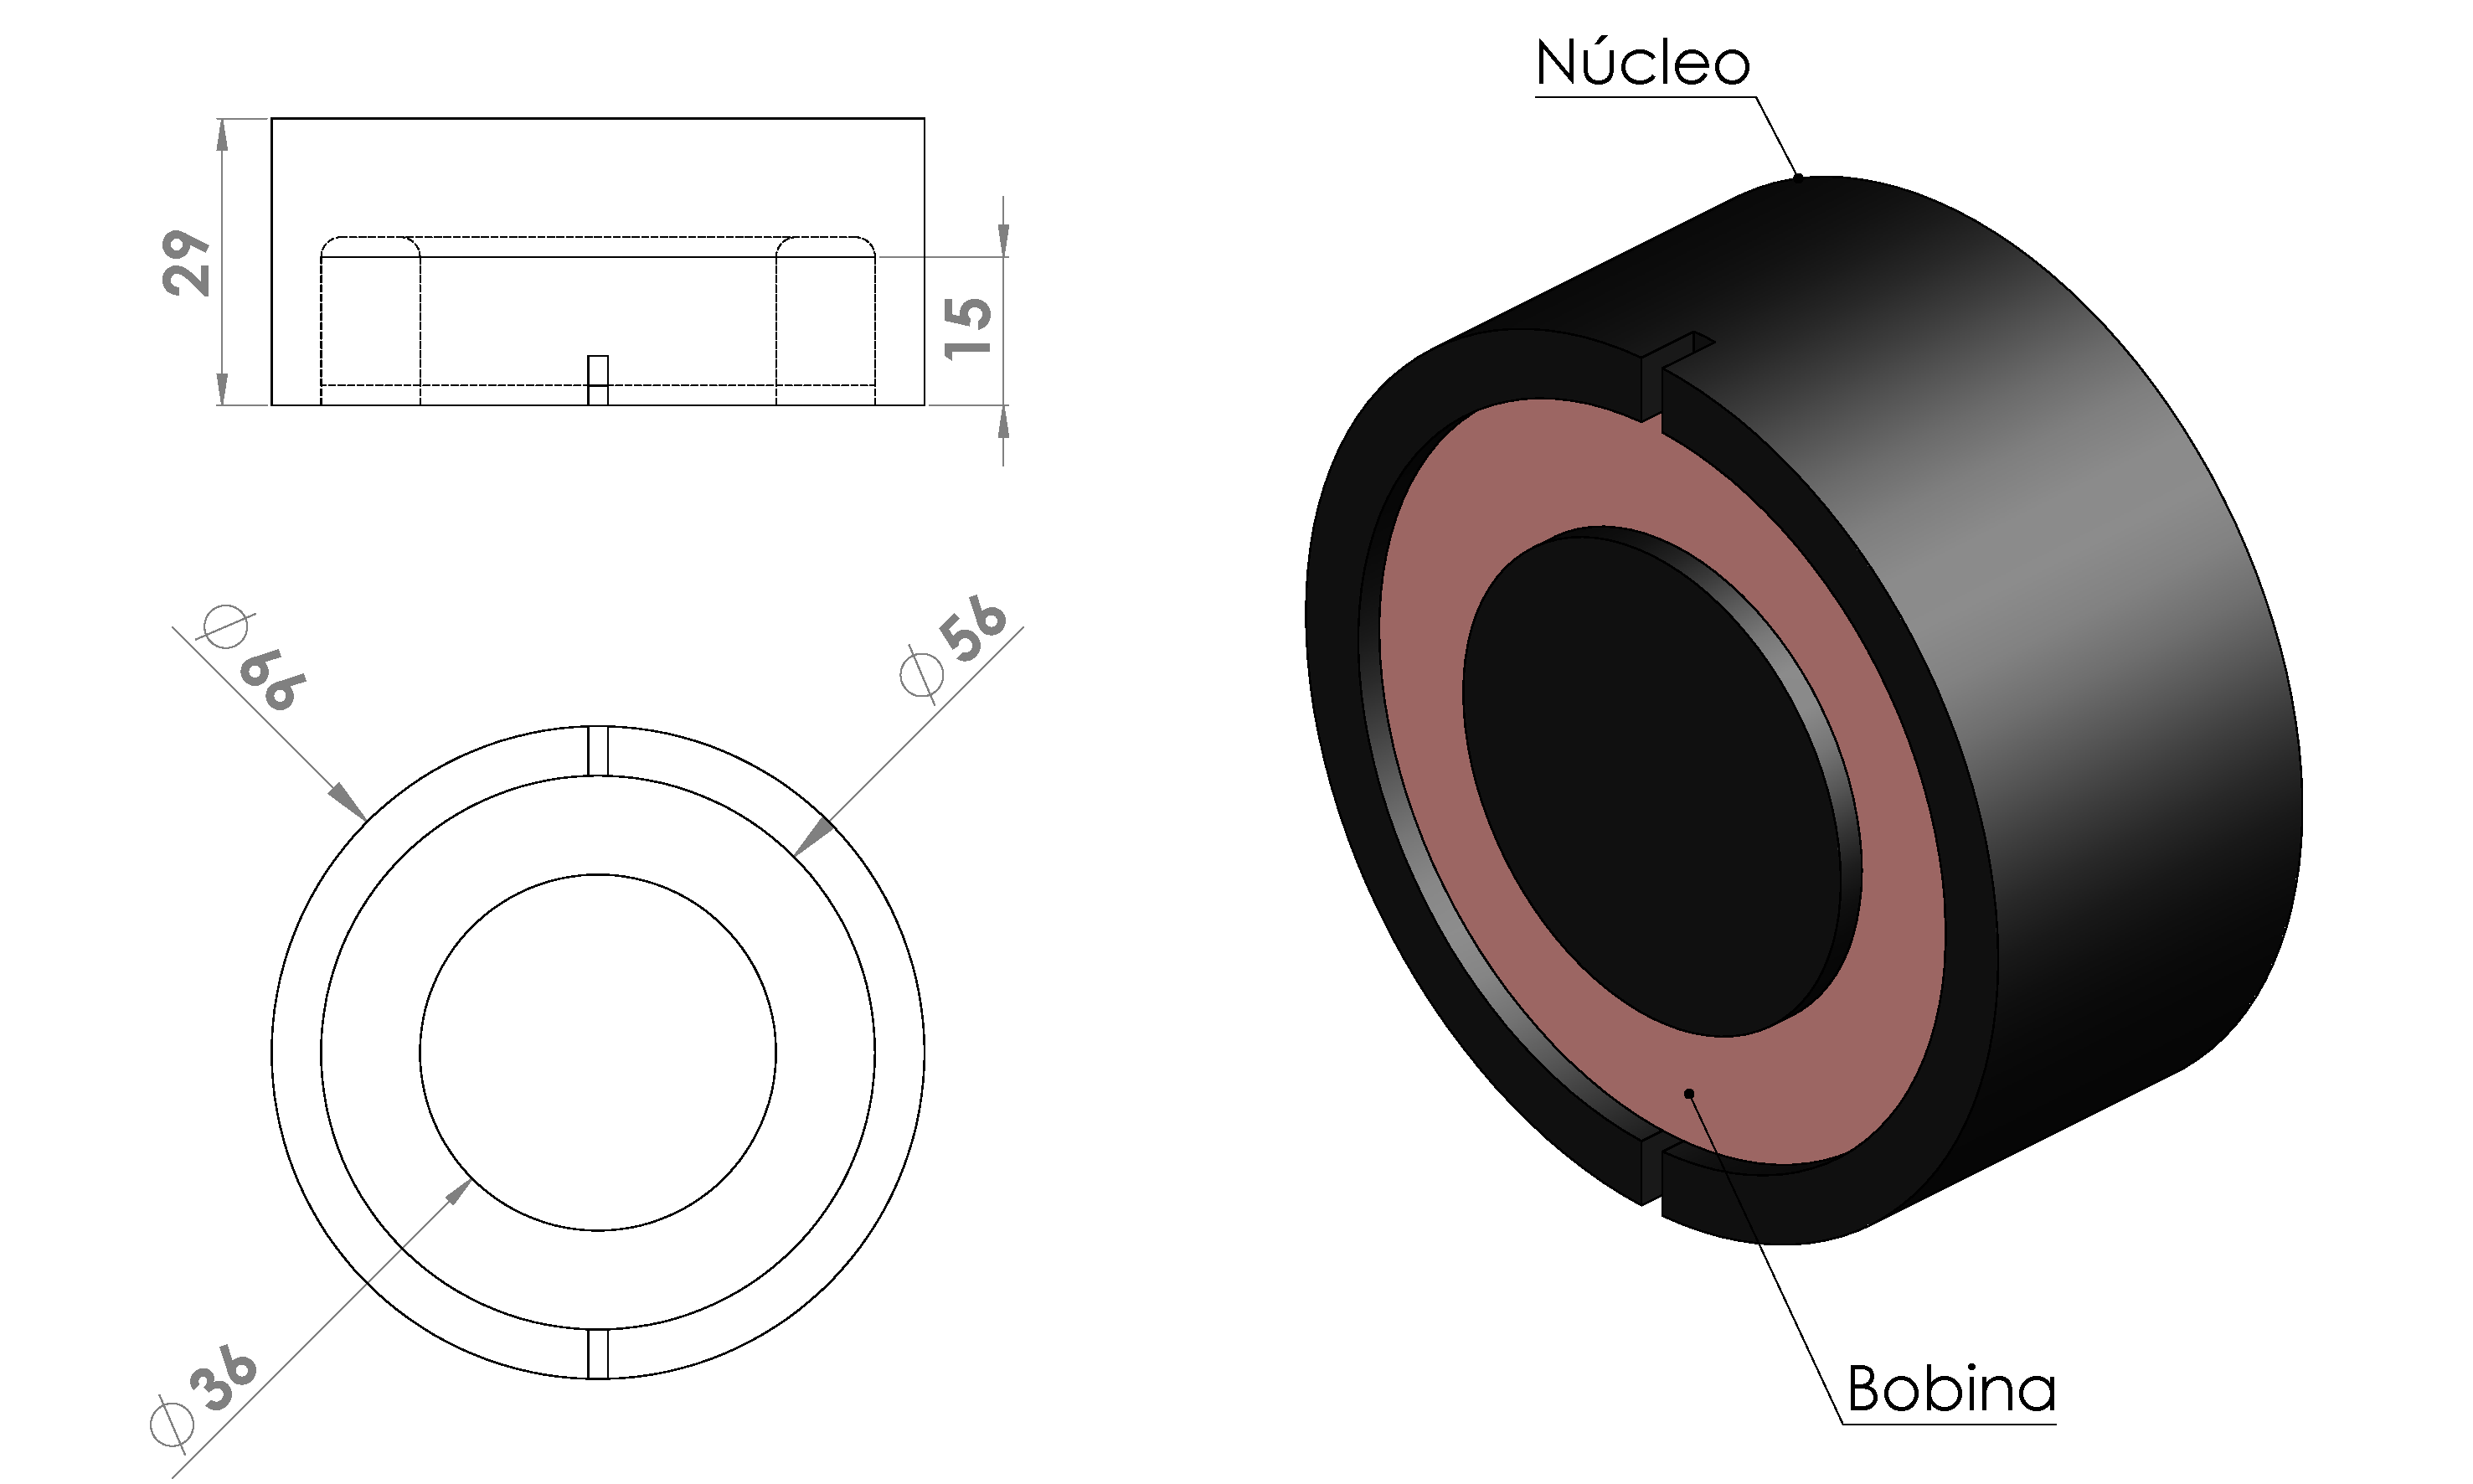
\includegraphics[width=0.8\textwidth]{images/Capitulo_3/EIA_ensamble}
    \caption{Dimensiones del Electroim�n Axial.}
\end{figure}

\subsection{Simulaci�n FEM}

Con el fin de validar los c�lculos y comprobar que el n�cleo no alcance su punto de saturaci�n, se realiz� una simulaci�n de elemento finito con ayuda del software FEMM donde se obtuvieron los siguientes resultados:

\begin{figure}[H]
    \centering
    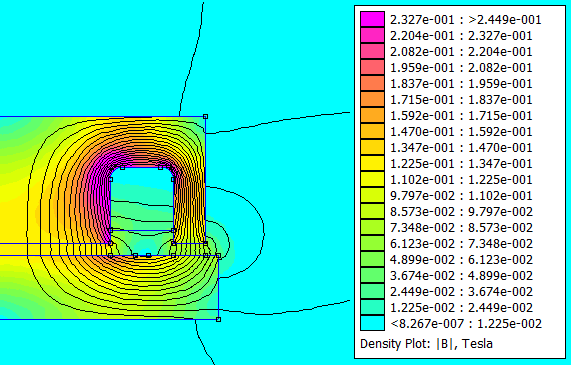
\includegraphics[width=0.8\textwidth]{images/Capitulo_3/simulacion_EIA_simple}
    \caption{Simulaci�n del electroim�n axial en FEMM.}
    \label{fig:simulacion-femm-axial}
\end{figure}

En la figura \ref{fig:simulacion-femm-axial} se puede observar que el valor m�ximo de inducci�n magn�tica es de $0.244 T$, lo cu�l est� por debajo del punto de saturaci�n del material. N�tese como las l�neas de flujo magn�tico se curvan en los l�mites del entrehierro, a esto se le conoce como flujo marginal y los efectos que causa sobre la fuerza del electroim�n se puede observar en la figura \ref{fig:curva-fuerza-rma}:

\begin{figure}[H]
    \centering
    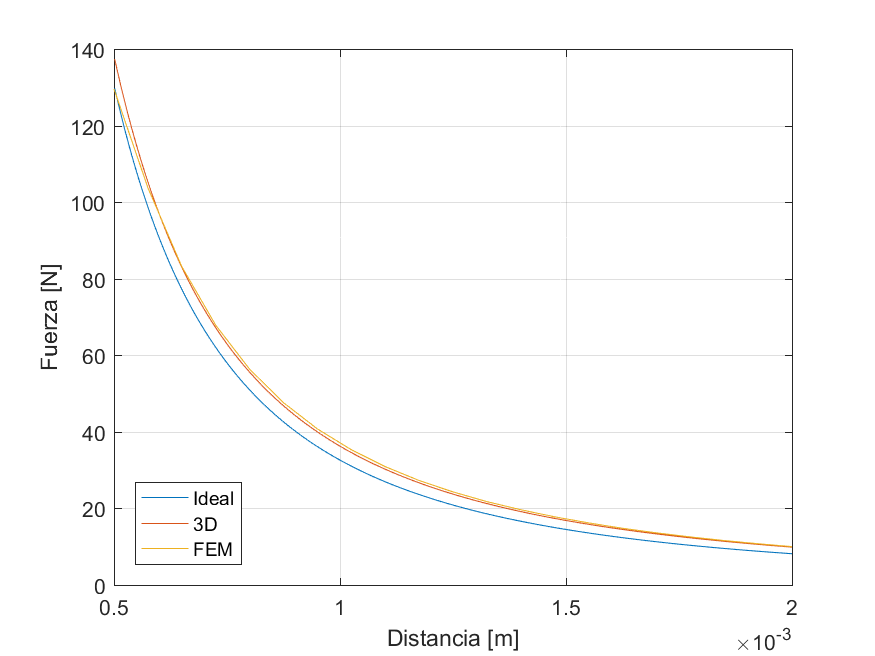
\includegraphics[width=0.8\textwidth]{images/Capitulo_3/simulacion_vs_modelo_axial}
    \caption{Curva Fuerza - Distancia del RMA.}
    \label{fig:curva-fuerza-rma}
\end{figure}

Cabe destacar que el modelado desarrollado en la secci�n \ref{sec:flujo-marginal}, el cual toma en cuenta los efectos del flujo marginal, coincide con los resultados de la simulaci�n FEM. 

\subsection{Electr�nica de accionamiento}

Como se mencion� anteriormente, se usar� la misma electr�nica de accionamiento que en el RMR. Sin embargo, debido a la diferencia en la inductancia de sus bobinas el sistema posee una respuesta en frecuencia distinta. 

Usando las f�rmulas \ref{eq:respuesta-frecuencia-accionamiento-1} y \ref{eq:respuesta-frecuencia-accionamiento-2} podemos determinar que la respuesta en frecuencia del electroim�n para diferentes valores de corriente resultan en la figura \ref{fig:respuesta-frecuencia-electroiman-RMA}.  

\begin{figure}[H]
    \centering
    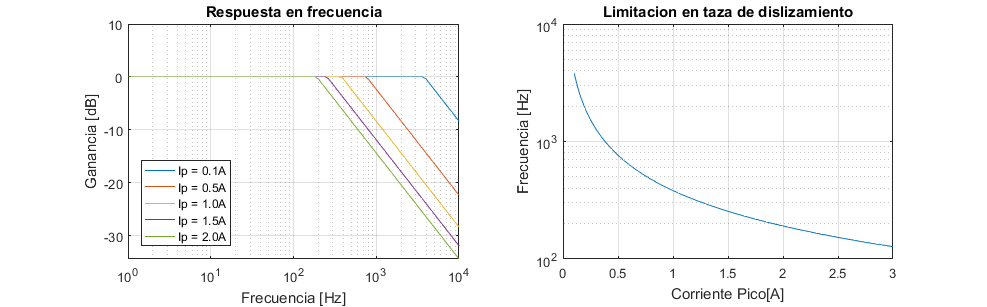
\includegraphics[width=\textwidth]{images/Capitulo_3/respuesta_dinamica_cp}
    \caption{Respuesta en frecuencia de la electr�nica de accionamiento RMA.}
    \label{fig:respuesta-frecuencia-electroiman-RMA}
\end{figure}

\newpage

\section{M�dulo de compensaci�n de carga est�tica}

Ante los problemas del alto consumo de corriente en los rodamientos magn�ticos activos, se propone una soluci�n con base en los principios de funcionamiento de los rodamientos magn�ticos pasivos, donde se opt� por utilizar un im�n permanente que deber� proveer un campo magn�tico base para reducir su consumo. 

El MCCE consiste en un im�n permanente cuya distancia al collar�n de levitaci�n es variada mediante un servomecanismo de retracci�n. De esta manera, se puede ejercer una fuerza cuasiconstante con un m�nimo consumo energ�tico. Este se conforma de: im�n permanente, n�cleo ferromagn�tico, mecanismo de retracci�n, motor y un circuito de accionamiento. El im�n permanente magnetiza todo el circuito, el n�cleo gu�a el flujo magn�tico y maximiza la fuerza que el im�n permanente puede ejercer. El mecanismo de retracci�n convierte el movimiento de rotaci�n del motor en movimiento lineal para el im�n permanente, y el circuito de accionamiento se encarga de controlar el motor. 

\begin{figure}[H]
    \centering
    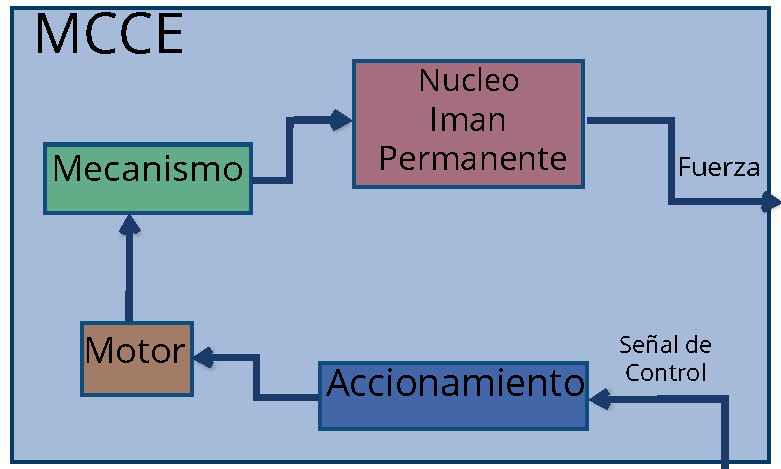
\includegraphics[width=0.625\textwidth]{images/Capitulo_3/diagrama_funcional_mcce}
    \caption{M�dulo de compensaci�n para cargas est�ticas.}
\end{figure}

\newpage

\subsection{An�lisis de consumo energ�tico} 

Como se indica en la secci�n \ref{sec:numero-polos}, el consumo en un electroim�n esta dado por:

\begin{equation}
P = (\frac{R F}{K_e}) \label{eq:consumo-electroiman}
\end{equation}

En la ecuaci�n \ref{eq:consumo-electroiman} se puede observar que el consumo depende de manera proporcionada a la fuerza aplicada por el electroim�n. Si descomponemos esta fuerza en sus componentes de Fourier tenemos un t�rmino constante y la suma de las componentes arm�nicas a diversas frecuencias.

El t�rmino constate que usualmente corresponde al peso del objeto representa la mayor parte la fuerza, y por lo tanto, de las p�rdidas. Eliminar esa componente de fuerza reducir�a la corriente y el consumo energ�tico total del rodamiento.

Usar un im�n permanente con fuerza $F_{ip}$ como en el caso de un rodamiento pasivo, reduce las p�rdidas del sistema a un valor de: 

\begin{equation}
|\frac{R (F_L - F_{ip})}{K}|
\end{equation}

El problema consiste en decidir de antemano el valor de la carga est�tica para igualar los t�rminos $F_l$ y $F_{ip}$, y as� reducir las p�rdidas. 

Es posible variar la fuerza que ejerce un im�n permanente variando la distancia entre este y el objetivo. Si usamos un im�n capaz de ejercer un fuerza $F_ip$ mucho m�s grande de la requerida y la montamos sobre una plataforma m�vil (mecanismo de retracci�n), podr�amos ajustar la fuerza hasta llevar las p�rdidas a $0$.  

\begin{figure}[H]
    \centering
    \begin{subfigure}[b]{0.4\textwidth}
        
\includegraphics[width=\textwidth]{images/Capitulo_2/iman_permanente}
        \caption{Im�n permanente.}
    \end{subfigure}
    ~ %add desired spacing between images, e. g. ~, \quad, \qquad, \hfill etc. 
      %(or a blank line to force the subfigure onto a new line)
    \begin{subfigure}[b]{0.4\textwidth}
        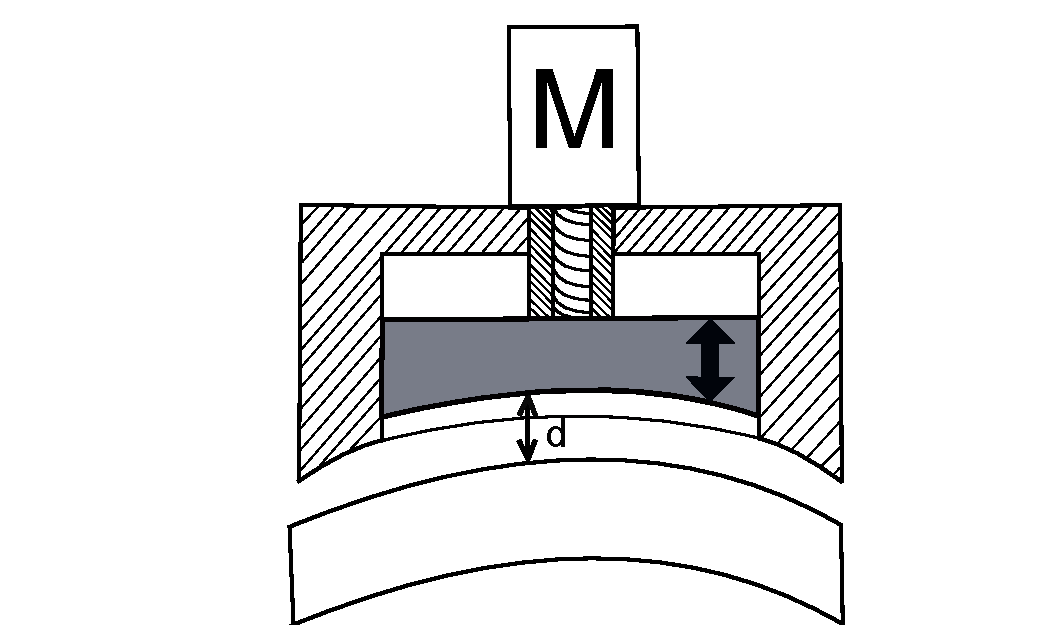
\includegraphics[width=\textwidth]{images/Capitulo_2/mecanismo_retraccion}
        \caption{Mecanismo de retracci�n.}
    \end{subfigure}
\end{figure}

\subsection{Im�n Permanente y N�cleo Ferromagn�tico}

La fuerza que ejerce un im�n permanente puede modelarse mediante la f�rmula:

\begin{equation}
	F = \frac{B_r^2}{2 \mu_0 (1 + (\frac{\mu_m}{\mu_0})(\frac{A_m}{A_g})(\frac{g}{l_m}))^2}[\frac{A_m + 2A_g}{2A_g}]
	\label{eq:fuerza-iman-permanente}
\end{equation}

Esta fuerza depende tanto de la geometr�a del im�n permanente como del material del que est� compuesto, y donde $H_c$, $B_r$ y $A_m$ son los t�rminos dominantes.  

Es nuestro objetivo dise�ar un conjunto im�n-n�cleo lo m�s peque�o posible, y debido a que las dimensiones y composici�n de los imanes permanentes est�n determinadas por el fabricante nos limitamos a seleccionar el im�n m�s peque�o disponible. Este im�n deber� generar al menos una fuerza $F_{min}$.   

Finalmente las dimensiones del n�cleo se determinan de tal manera que el im�n permanente pueda instalarse dentro de �ste.  

Para el dise�o del im�n tenemos el siguiente proceso:

\begin{enumerate}
\item Especificar las condiciones de operaci�n $F_{min}$, $y_{min}$. 
\item Seleccionar el material del im�n permanente con el $H_c$, $B_r$ m�s altos disponibles. 
\item Seleccionar las dimensiones del im�n permanente seg�n disponibilidad del fabricante. 
\item Dimensionar el n�cleo gu�a de manera que acomode correctamente el im�n permanente. 
\item Usar la f�rmula \ref{eq:fuerza-iman-permanente} para calcular la fuerza $F_{ip}$. 
\item Si la fuerza $F_{min} > F_{ip}$ incrementar las dimensi�n y repetir los pasos.
\end{enumerate}

\subsubsection{Selecci�n del im�n permanente}

Entre las diferentes composiciones de imanes permanentes destacan aquellas de Neodimio-Hierro-Boro, com�nmente conocidas como imanes de neodimio. Los valores m�s altos $H_c$ y  $B_r$ son alcanzados por los imanes de grado $N52$, con valores de $B_r = 1400mT$ y $H_c=796kA/m$ [v�ase anexo B]. 

Siguiendo el procedimiento anterior para generar una fuerza $F_{min}$ de al menos $50 N$ result� en un im�n c�bico de 10 mm por lado \cite{cite_s21_2017_first4magnets}.

As� pues el conjunto Im�n Permanente - N�cleo Ferromagn�tico queda representado por la figura \ref{fig:conjunto-ip-nucleo}.

\begin{figure}[H]
    \centering
    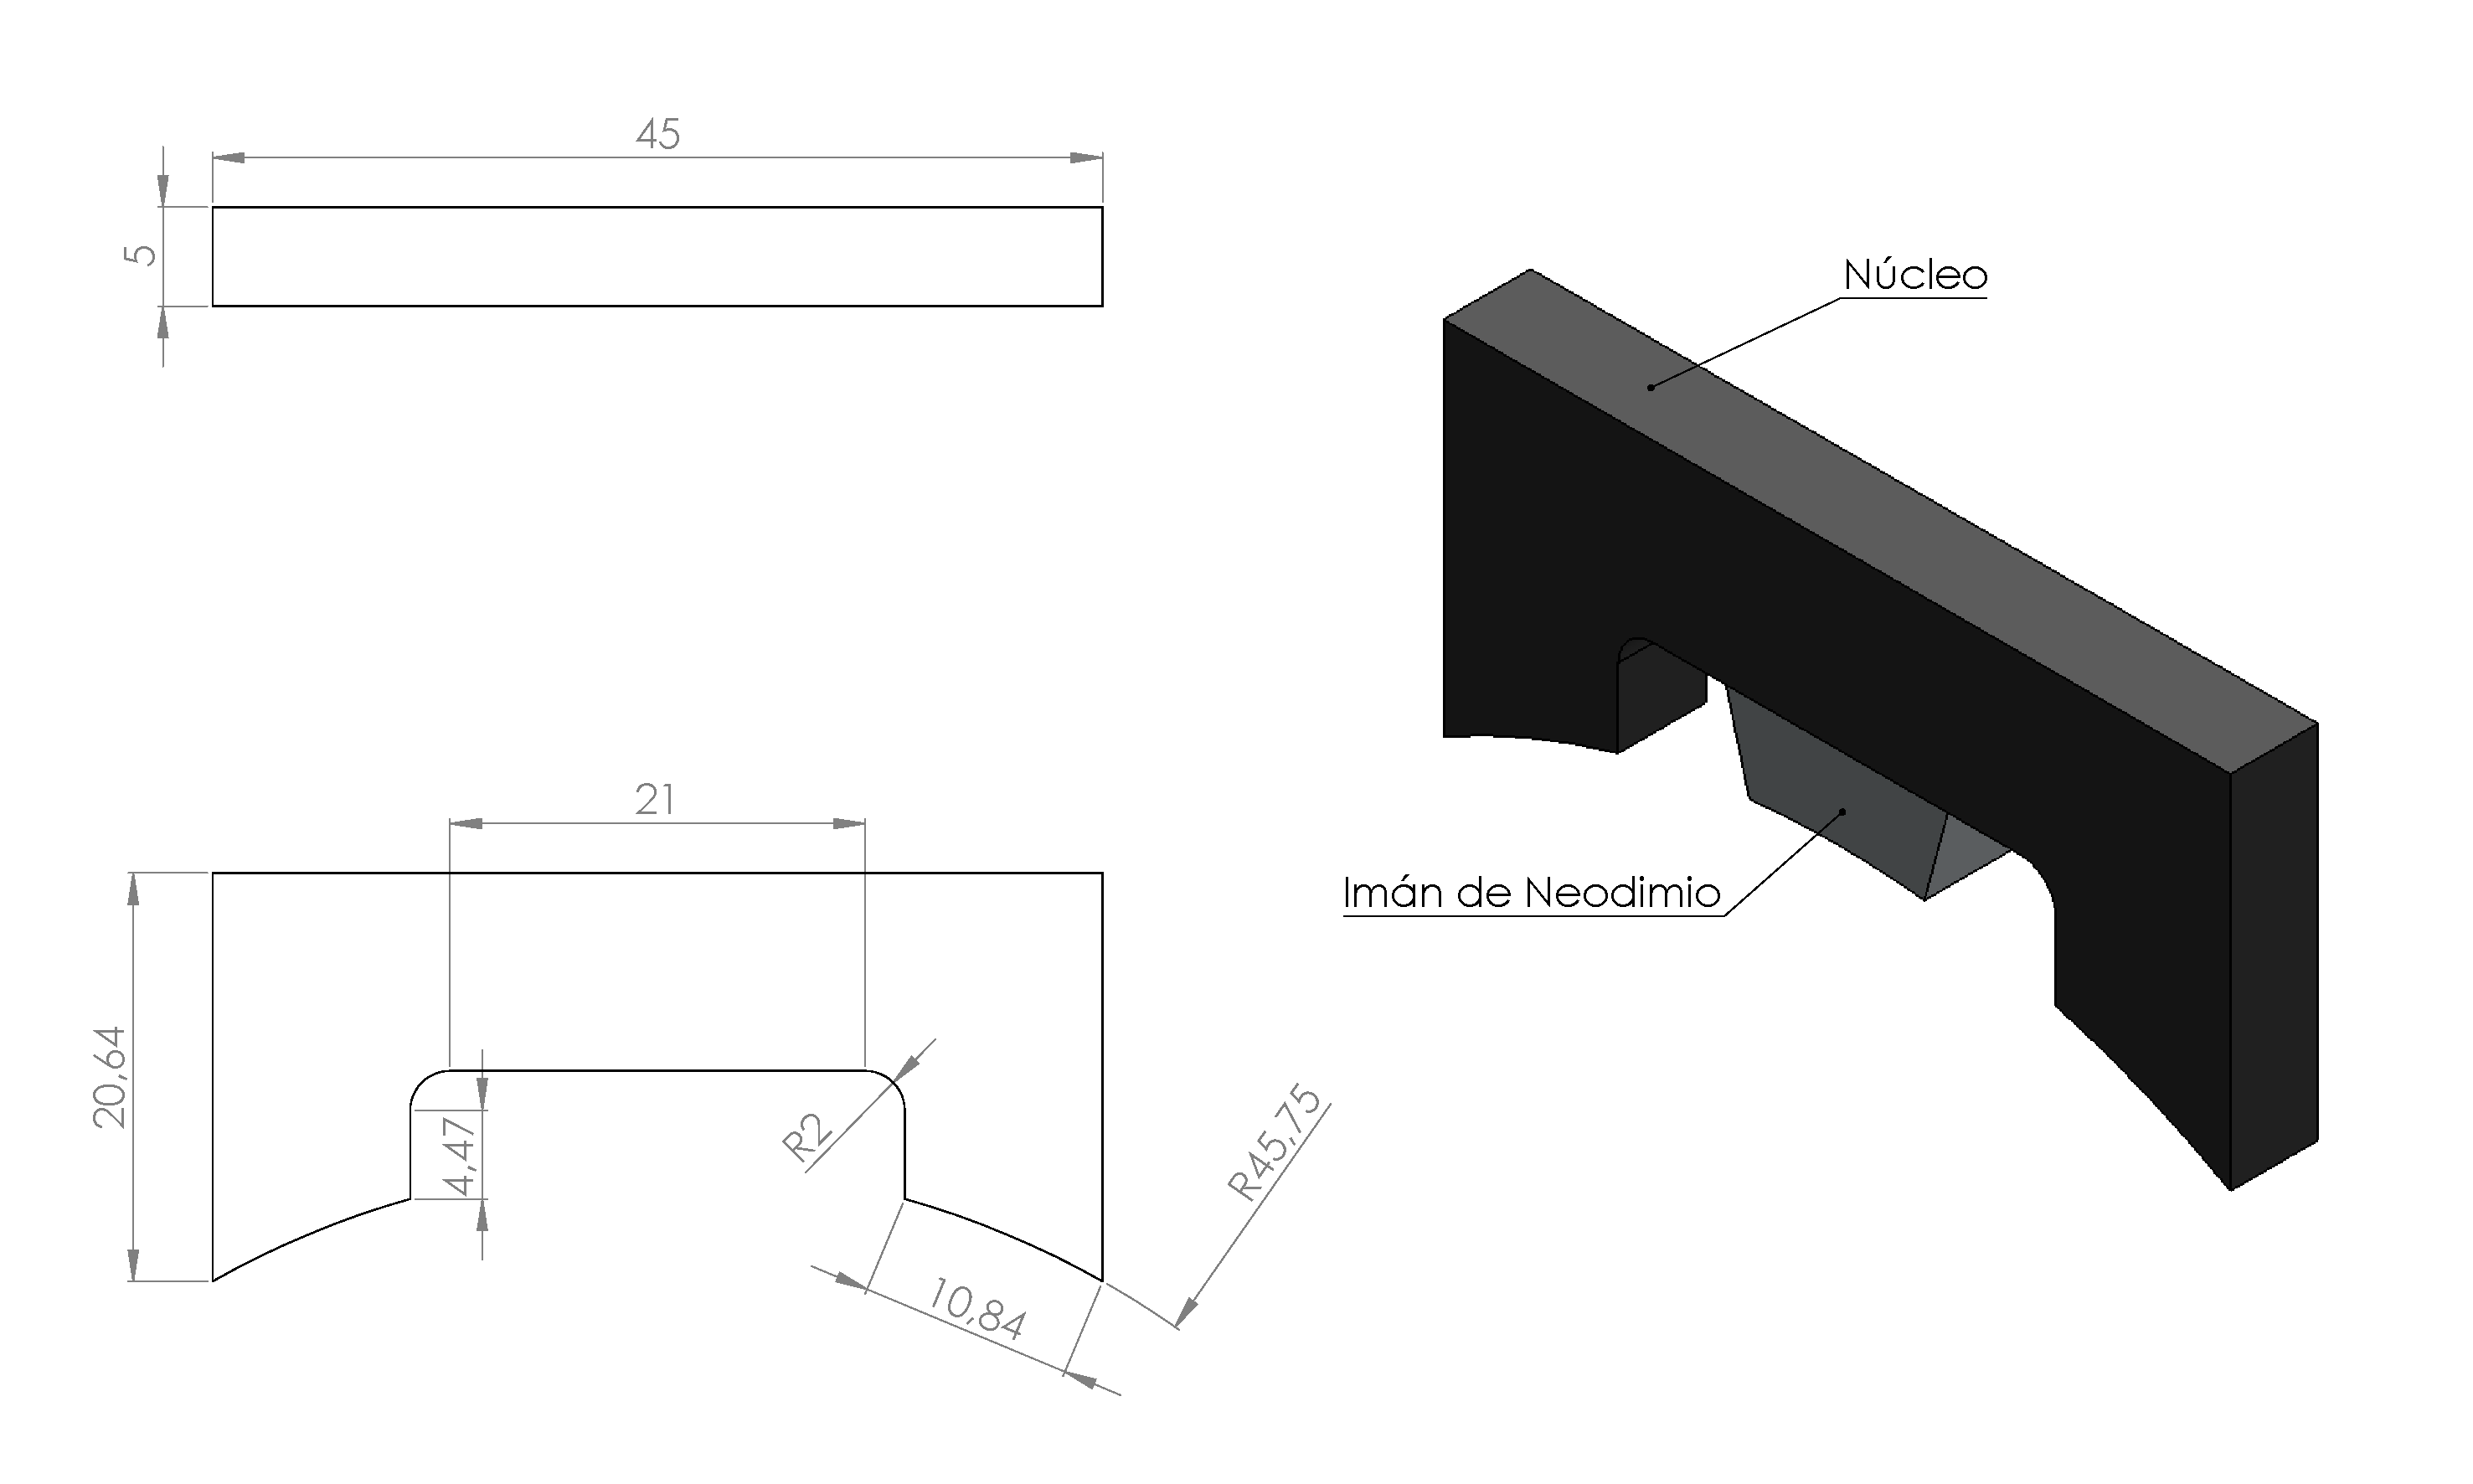
\includegraphics[width=0.8\textwidth]{images/Capitulo_3/IP_ensamble}
    \caption{Conjunto Im�n permanente - N�cleo Ferromagn�tico.}
    \label{fig:conjunto-ip-nucleo}
\end{figure}

\subsubsection{Simulaci�n FEM}

As� como se hizo en la secci�n \ref{sec:simulacion-fem-electroiman}, podemos validar nuestro modelo mediante una simulaci�n FEM, lo que resulta en la siguiente curva caracter�stica de la figura \ref{fig:iman-permanente-curva}.

\begin{figure}[H]
\begin{center}
\centering
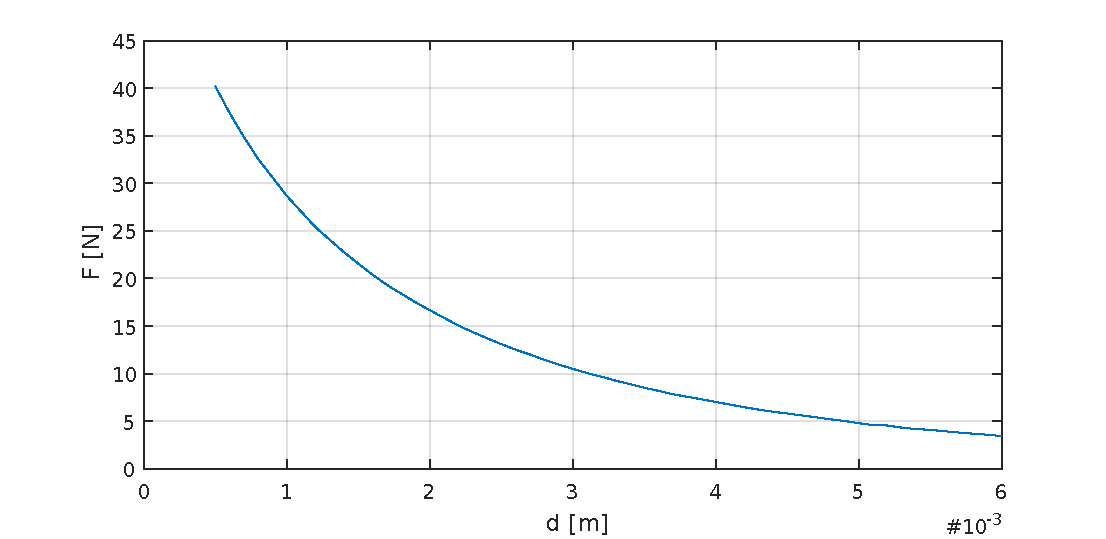
\includegraphics[width=0.8\textwidth]{images/Capitulo_3/fuerza_iman_permanente}
\caption{Curva caracter�stica del im�n permanente.}
\label{fig:iman-permanente-curva}
\end{center}
\end{figure}

\subsection{Mecanismo de retracci�n}

El servomecanismo que utilizar� el im�n permanente para su desplazamiento consiste en un par de rieles que se montar�n sobre la base del motorreductor y la base del im�n permanente; esta �ltima ser� la que se desplazar� a lo largo de los rieles. 

Para generar dicho desplazamiento se utiliza un mecanismo tornillo-tuerca, conocido tambi�n como husillo-tuerca. Es un mecanismo de transformaci�n circular a lineal compuesto por una tuerca alojada en un eje roscado (tornillo).

\begin{figure}[H]
\centering
	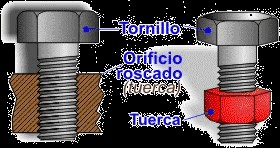
\includegraphics[scale=.3]{images/Capitulo_3/Tornillo}
	\caption{\textit{Mecanismo Tornillo Tuerca \citep{cite_17}.}}
\end{figure}

Este mecanismo se puede plantear de dos formas: un tornillo de posici�n fija que al girar provoca el desplazamiento de la tuerca, o una tuerca fija que produce el desplazamiento del tornillo cuando este gira. En este caso, utilizaremos el tornillo de posici�n fija y la tuerca consistir� en la base del im�n permanente. 
Este tipo de mecanismos son utilizados en diferentes aplicaciones y son ideales como mecanismos de desplazamiento, debido en parte a su gran precisi�n y al reducido espacio que requieren. 
El avance depende de dos factores \citep{cite_18} :

\begin{itemize}
\item La velocidad de giro del elemento motriz.
\item El paso de la rosca del tornillo. Cuanto mayor sea el paso, mayor ser� la velocidad de avance.
\end{itemize}

\subsubsection{Selecci\'on de la Rosca}

El mecanismo tornillo-tuerca presenta una ventaja muy importante respecto a otros sistemas de conversi�n de movimiento circular en longitudinal: por cada vuelta del tornillo la tuerca solamente avanza la distancia correspondiente al paso de la rosca. 

En general el avance del tornillo viene dado por:

\begin{equation}
A = p * e
\end{equation}

Donde $p$ es el paso de la rosca y $e$ corresponde al n�mero de entradas del tornillo. 

Con el fin de reducir la fuerza producida por el im�n permanente hasta un valor m�nimo, se necesita un recorrido de 4 mm respecto a la distancia m�nima entre �ste y el collar�n de levitaci�n. Con estas consideraciones se determin� el uso de una rosca m�trica M 2 x 0,4, que corresponde a un di�metro nominal de 2 mm, paso de rosca de 0.4 mm y una entrada [v�ase anexo A], con lo que �nicamente requerir�amos generar 10 vueltas del motorreductor para el desplazamiento m�ximo de 4 mm. 

\begin{figure}[H]
\centering
		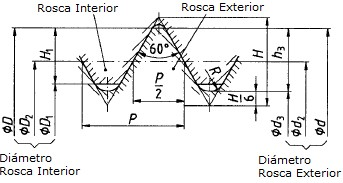
\includegraphics[width=0.5\textwidth]{images/Capitulo_3/Rosca}
		\caption{\textit{Especificaciones de la rosca M 2 x 0.4 \citep{cite_19}.}}
\end{figure}

Especificaciones \citep{cite_19}:

\begin{itemize}
\item Di�metro nominal: $D$ = $d$ = $2 mm$
\item Paso: $P$ = $0.4 mm$
\item Altura: $H$ = $\frac{raiz*3}{2}$*$P$ = 0.866025*$P$ = $0.35 mm$
\item Profundidad portante de flancos: $H1$ = ($D$ - $D_1$)/2 = 5/8*$H$ = 0.541266*$P$ = $0.22 mm$
\item Profundidad de rosca: $h_3$ = ($d$ - $d_3$)/2 = 17/24*$H$ = 0.613435*$P$ = $0.25 mm$
\item Di�metro de francos: $D2$ = $d_2$ = $d$ - 3/4*$H$ = $d$ - 0.649519*$P$ = $1.74 mm$
\item Radio fondo de rosca: $R$ = $H$/6 = 0.144338*$P$ = $0.058 mm$
\end{itemize}

Rosca Interior (Tuerca):
\begin{itemize}
\item $D_1$ = $d_2$ - 2*($H$/2 - $H$/4) = d - 2*$H_1$ = $d$ - 1.082532*$P$ = $1.57 mm$
\end{itemize}

Rosca Exterior (Tornillo):
\begin{itemize}
\item Di�metro del n�cleo: $d_3$ = $d_2$ - 2*($H$/2 - $H$/6) = $d$ - 1.226869*$P$ = $1.51 mm$
\item Di�metro del n�cleo: $d_3$ = $d_1$ - $H$/6 = $1.51 mm$ (seg�n la norma DIN ISO 724)
\end{itemize}

\subsubsection{Motorreductor} \label{sec:Motorreductor}

Para el motorreductor se seleccion� el modelo \textbf{LP 6V 1000:1} de Pololu \cite{cite_s19_2017_polulu}. Este motorreductor miniatura de alto par tiene una caja de cambios de $1000: 1$, por lo que es una gran opci�n para aplicaciones que requieren un control preciso a velocidades muy bajas. Estas unidades tienen un eje de salida en forma de D de $3 mm$ de di�metro.

Este motorreductor posee unas especificaciones clave de $14 RPM @ 6 V$ y $40 mA$ al vac�o, $5 kg-cm$ de par y $0.36 A$ en bloqueo.

Estos motores est�n dise�ados para poder operar a $6 V$, aunque en general, estos tipos de motores pueden funcionar a voltajes por encima y por debajo de este voltaje nominal, por lo que deber�an funcionar c�modamente en el rango de $3 - 9 V$. 
 
    \begin{figure}[H]
    \centering
        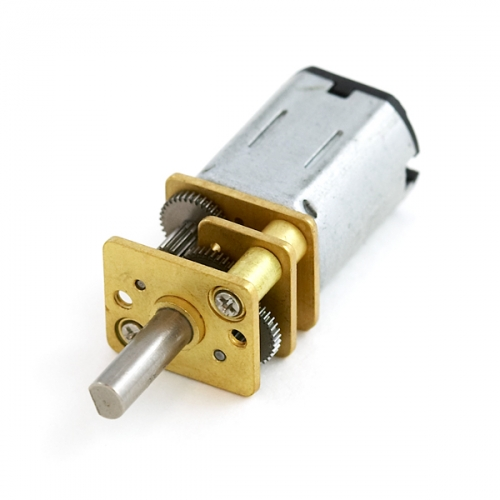
\includegraphics[width=0.3\textwidth]{images/Capitulo_3/motoreductor}
        \caption{Motorreductor.}
    \end{figure}
    
\newpage

Finalmente el ensamble del MCCE queda ilustrado en la figura \ref{fig:configuracion-final-MCCE}.

\begin{figure}[H]
    \centering
    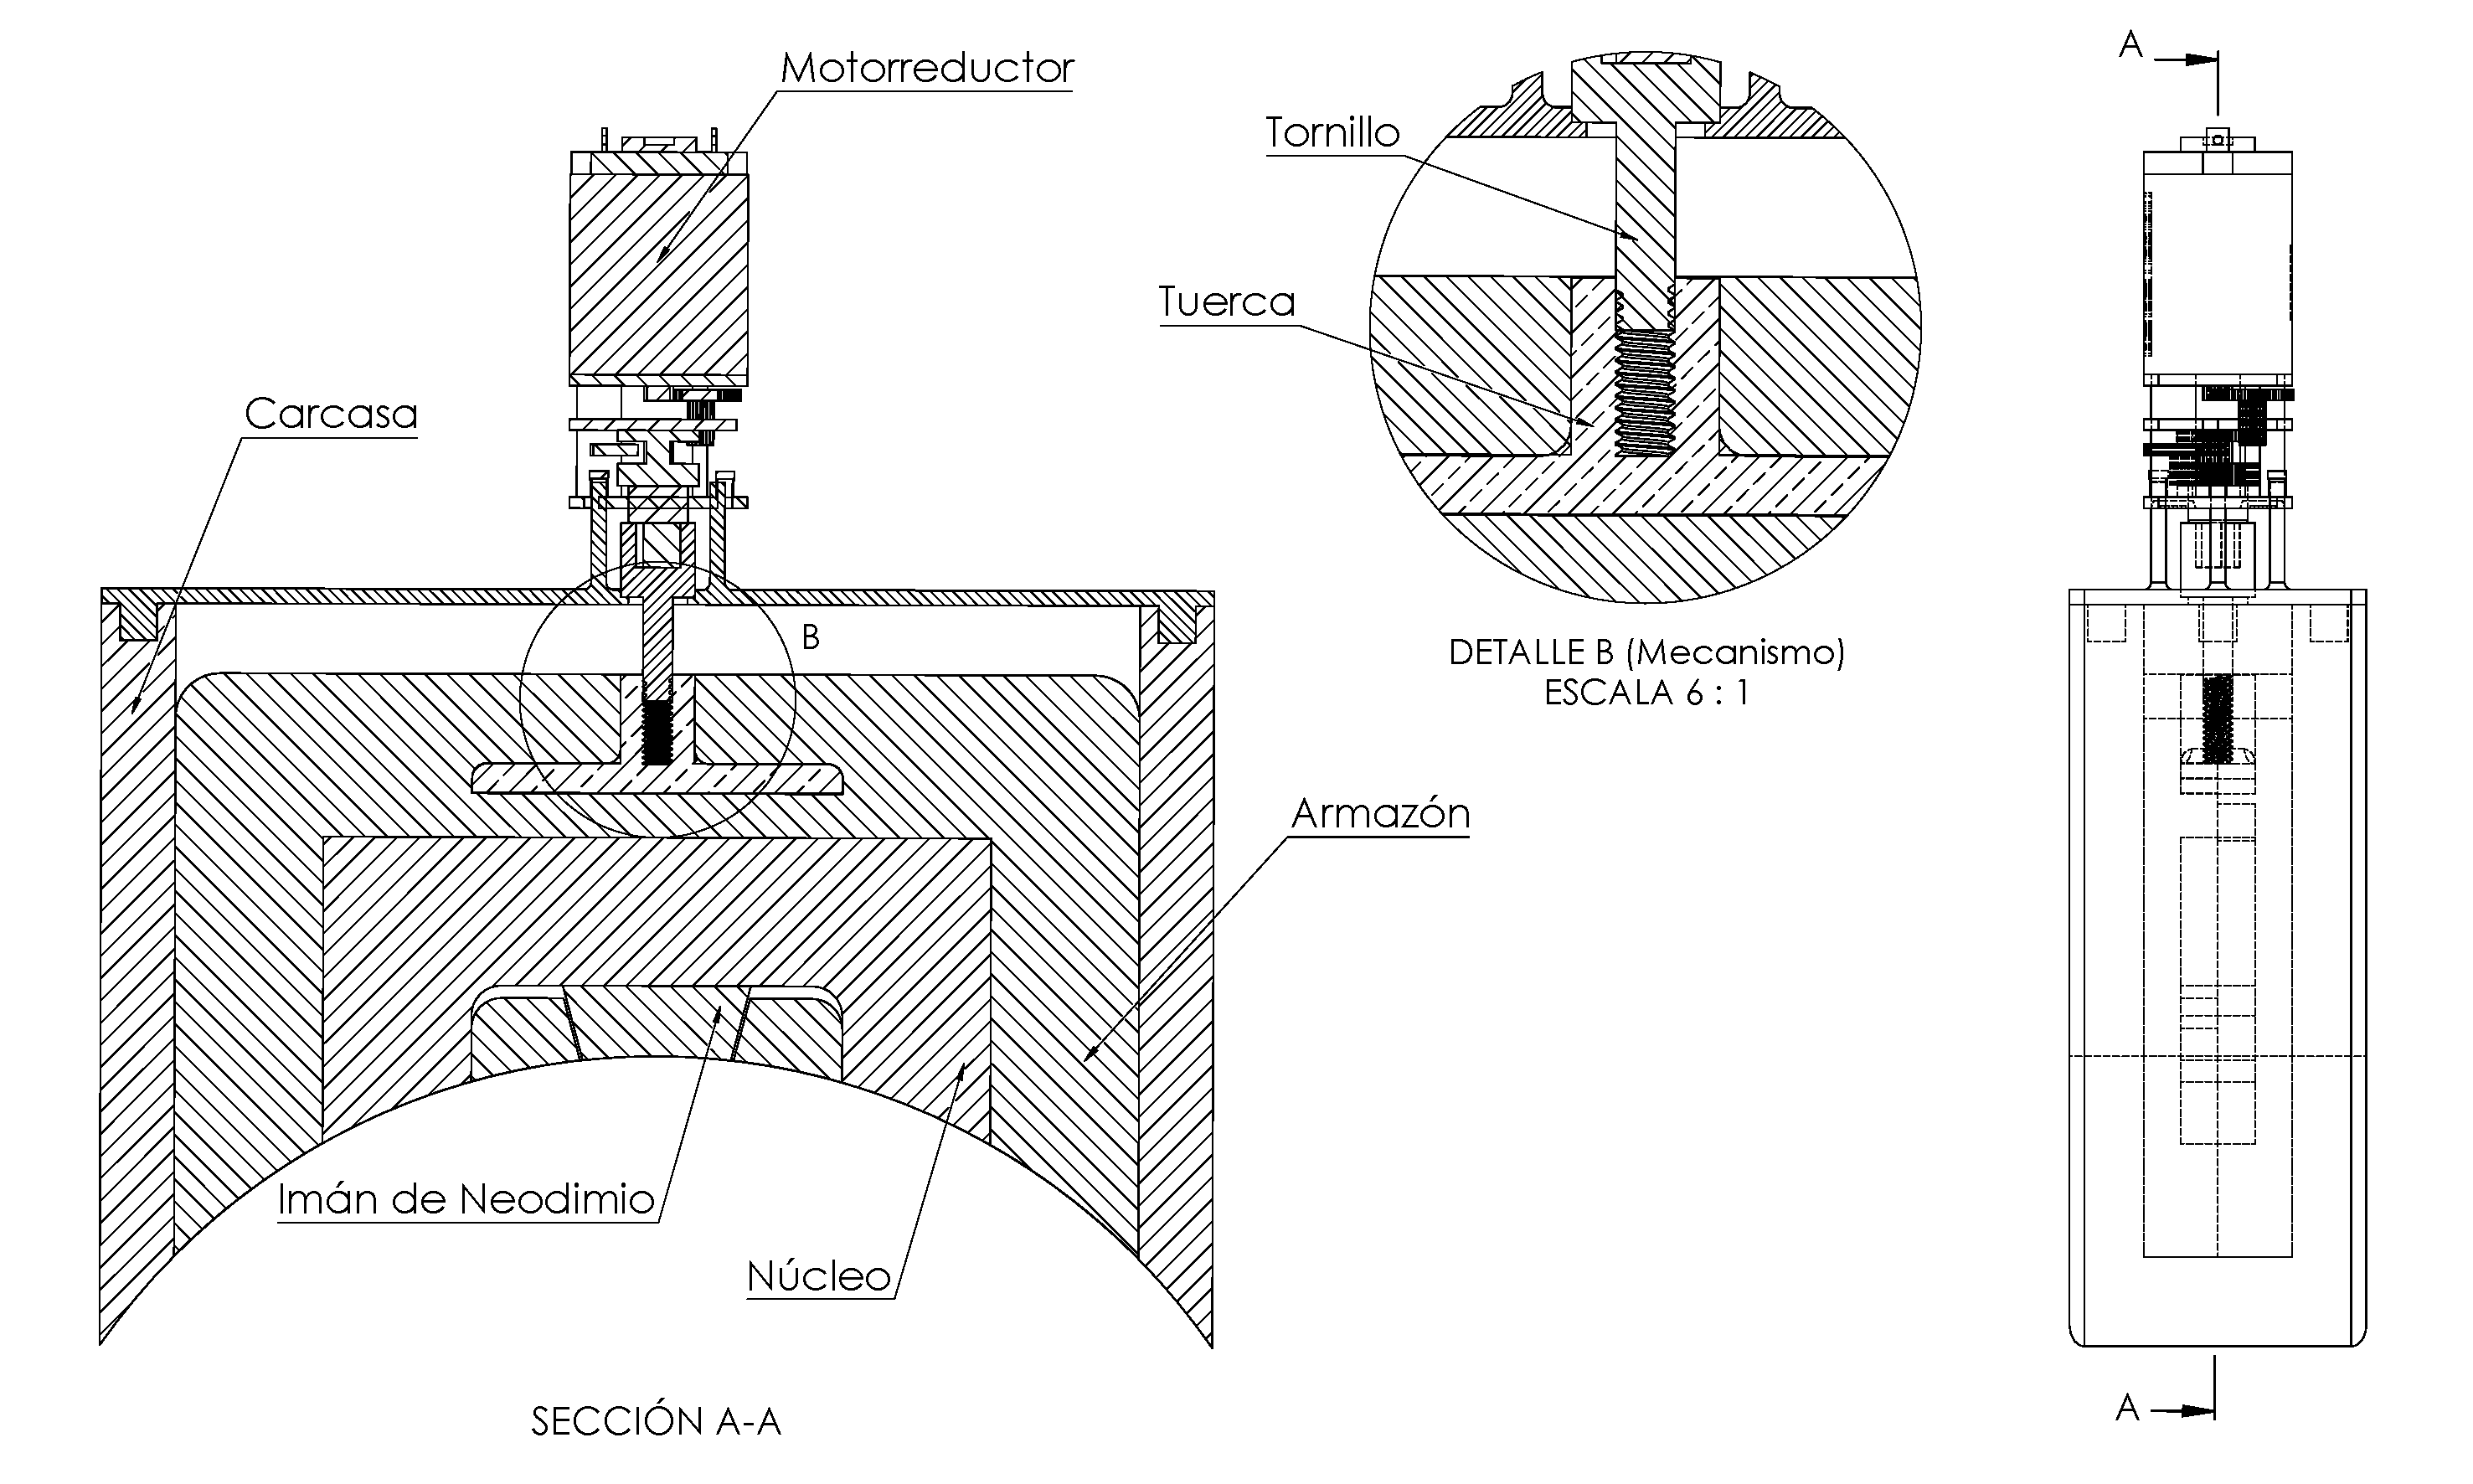
\includegraphics[width=\textwidth]{images/Capitulo_3/Mecanismo_ensamble}
    \caption{Configuraci�n final MCCE.}
    \label{fig:configuracion-final-MCCE}
\end{figure}

\subsection{Accionamiento}

Como se indica en la secci�n \ref{sec:Motorreductor}, la corriente m�xima que demanda el motor es de $360 mA$. Como queremos mover el motor en ambas direcciones es necesario un circuito de puente H para su accionamiento. Para ello se seleccion� el circuito integrado L293 \cite{cite_s18_2017_l293}. 

Este controlador de motor cuenta con dos puentes H que se pueden utilizar para el control bidireccional de dos motores de corriente continua o para controlar un solo motor de pasos. Funciona a partir de $4.5$ a $36 V$ y puede entregar una corriente pico de $1 A$ por canal. La conexi�n de este circuito integrado se muestra en la figura \ref{fig:puente-h-l293}.

\begin{figure}[H]
    \centering
    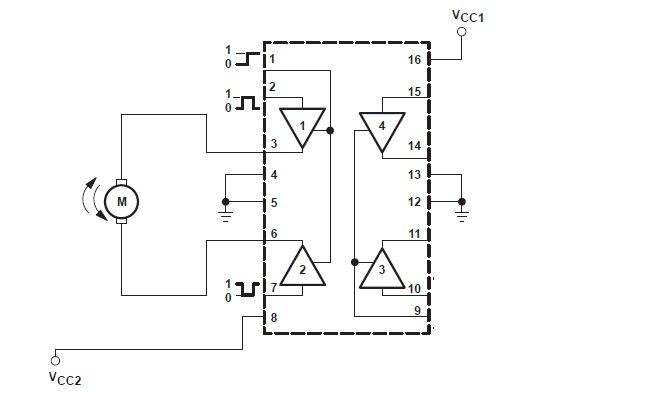
\includegraphics[width=0.7\textwidth]{images/Capitulo_3/CircuitoL293}
    \caption{Circuito Puente H L293.}
    \label{fig:puente-h-l293}
\end{figure}

\subsection{Modelado electromec�nico}

Para el modelado del MCCE comenzamos por establecer las ecuaciones \ref{eq:motor-MCCE-1}, \ref{eq:motor-MCCE-2} y \ref{eq:motor-MCCE-3} correspondientes al motor de DC, donde la entrada del sistema es el voltaje de alimentaci�n $V{in}$ y como salidas tenemos el par de accionamiento $T_1$.

\begin{figure}[H]
\begin{center}
\centering
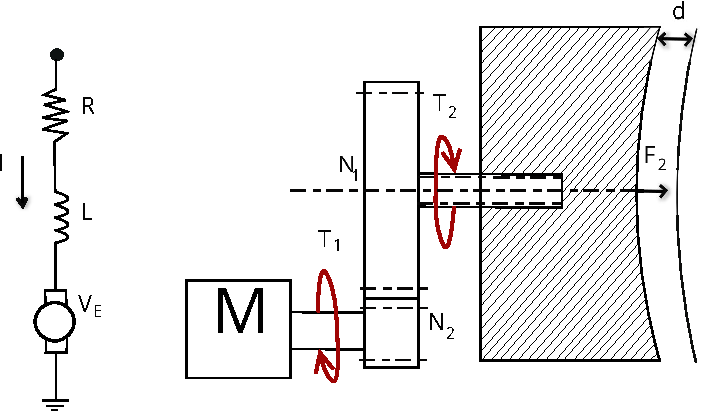
\includegraphics[width=8cm]{images/Capitulo_2/modelo_electromecanico_mcce}
\caption{Modelo electrodin�mico del MCCE.}
\end{center}
\end{figure}

Comenzamos con la malla del motor que describe la raz�n de cambio en la corriente:

\begin{equation}
 V_{in} = Ri + L \frac{d}{dt}i + V_{E}  
 \label{eq:motor-MCCE-1}	
\end{equation}

Seguimos con el par torsor de salida que es proporcional a la corriente del motor:

\begin{equation}
 T = K_t i 
 \label{eq:motor-MCCE-2}	
\end{equation}

Y finalmente el voltaje contraelectromotriz, el cual es proporcional a la velocidad del motor:
 
\begin{equation}
 V_{E} = K_v \omega 
  \label{eq:motor-MCCE-3}	
\end{equation}

A continuaci�n modelamos la parte mec�nica para relacionar el par del motor con la fuerza de elevaci�n del mecanismo. En los engranajes del motor tenemos una relaci�n de engranes de $N_1/N_2$, entonces las velocidades angulares ser�n:

\begin{equation}
 \omega_2 = \frac{N_2}{N_1} \omega_1
\end{equation}

Y la relaci�n de los pares torsores ser�: 

\begin{equation}
 T_2 = \frac{N_1}{N_2} T_1
\end{equation}

Finalmente, se relaciona el par torsor con la fuerza de elevaci�n y descenso del tornillo. Debido a la acci�n de la fricci�n se tiene una ecuaci�n para el descenso y otra para la elevaci�n. Para el par de elevaci�n tenemos:

\begin{equation}
    T = \frac{F \cdot d_m}{2} \cdot \frac{\rho + (\pi \cdot \mu \cdot d_m \cdot \sec \theta)}{(\pi \cdot d_m) - (\mu \cdot \rho \cdot  \sec \theta)} 
\end{equation}

Donde: \\
    $F$ = Valor de la carga\\
    $\rho$ = Paso del tornillo \\
    $d_m$ = Di�metro medio del tornillo\\
    $\mu$ = Coeficiente de rozamiento la rosca y el tornillo \\
    $\theta$ = $\frac{Angulo;de;la;rosca}{2}$\\

Y para el par de descenso tenemos:

\begin{equation}
    T= \frac{F \cdot d_m}{2} \cdot \frac{\pi \cdot \mu \cdot d_m \cdot \sec \theta - \rho}{\pi \cdot d_m + \mu \cdot \rho \cdot \sec \theta}
\end{equation}

Todas estas ecuaciones se introducen en el modelo de \textbf{Simulink} que queda representado en la figura \ref{fig:modelo-simulink-mcce}.

\begin{figure}[H]
\begin{center}
\centering
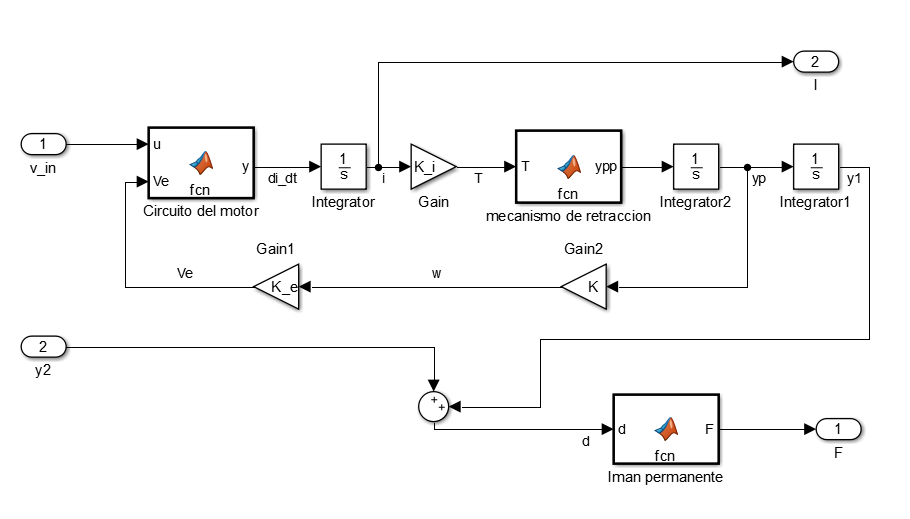
\includegraphics[width=\textwidth]{images/Capitulo_2/simulink_mcce}
\caption{Modelo en \textbf{Simulink} del MCCE.}
\label{fig:modelo-simulink-mcce}
\end{center}
\end{figure}

\newpage

\section{Sensor de distancia capacitivo}

El sensor de distancia capacitivo sirve para medir la posici�n del rotor dentro del rodamiento. Este sensor consiste en un electrodo y un circuito de acondicionamiento. 

El electrodo proyecta un campo el�ctrico al frente de este y la interacci�n del rotor con este campo causa cambios en la capacitancia que son convertidos a una se�al de frecuencia variable por el circuito de acondicionamiento.

\begin{figure}[H]
    \centering
    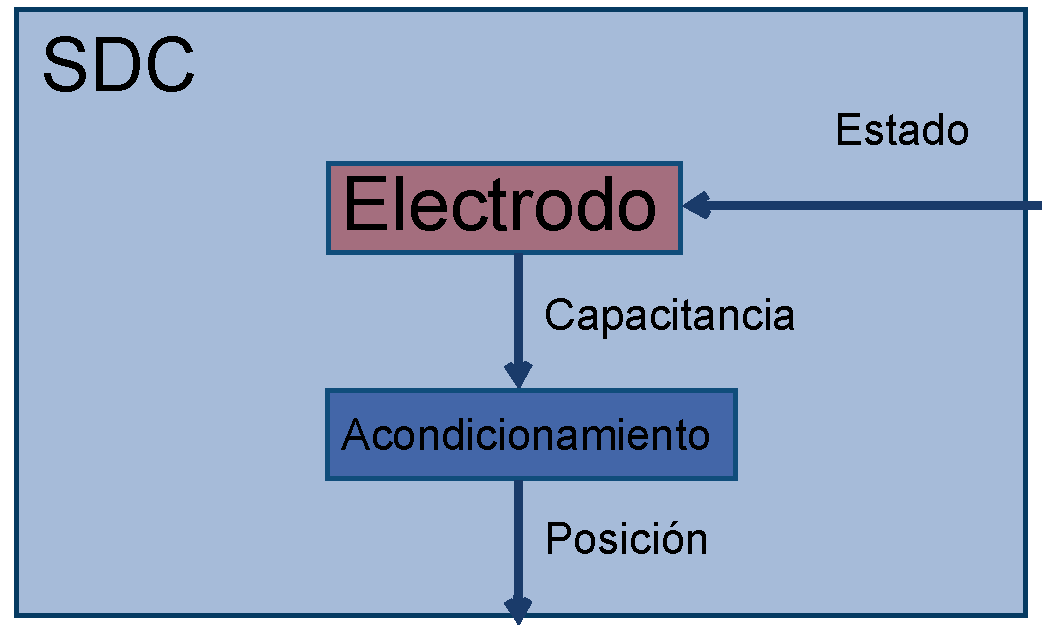
\includegraphics[width=0.625\textwidth]{images/Capitulo_3/diagrama_funcional_sdc}
    \caption{Sensor de distancia capacitivo (SDC).}
\end{figure}

Este sensor presenta ventajas como: 

\begin{enumerate}
	\item Un rango de operaci�n de $0.5 mm$ a $2mm$.
	\item Medici�n sin contacto. 
	\item Inmunidad al ruido de acoplamiento magn�tico causado por los electroimanes.
	\item R�pida respuesta.
\end{enumerate}

Para el sensor se utiliz� un dise�o similar al presentado en \citep{cite_14}, con la diferencia de que el circuito de acondicionamiento se encuentra embebido dentro de la  carcasa del electrodo, esto con el fin de eliminar los efectos de la capacitancia par�sita producidos e introducidos por el cable coaxial, adem�s dado que la carcasa act�a como blindaje se previenen interferencias externa de tipo el�ctrico.

\begin{figure}[H]
    \centering
    \begin{subfigure}[b]{0.45\textwidth}
     \centering
        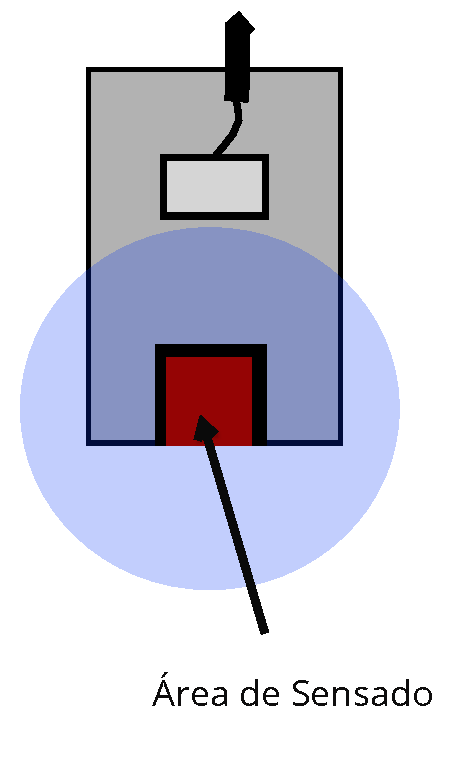
\includegraphics[width=.5\textwidth]{images/Capitulo_3/Sensor-ilustrativo-2}
        \caption{Sensor sin blindaje activo.}
    \end{subfigure}
    ~ %add desired spacing between images, e. g. ~, \quad, \qquad, \hfill etc. 
      %(or a blank line to force the subfigure onto a new line)
    \begin{subfigure}[b]{0.45\textwidth}
     \centering
        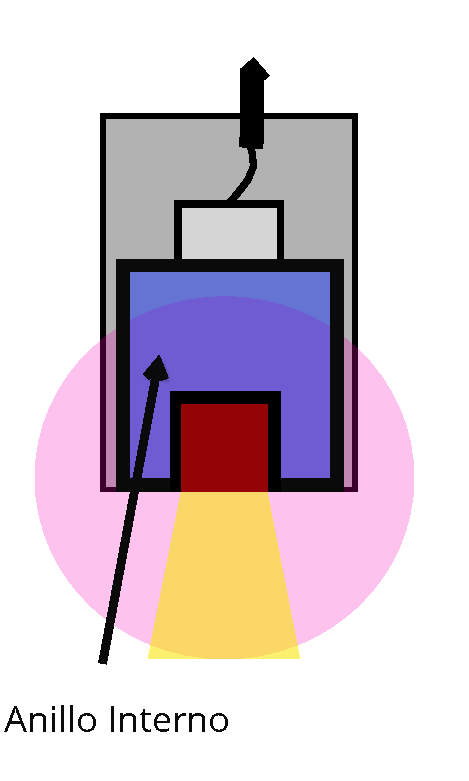
\includegraphics[width=.5\textwidth]{images/Capitulo_3/Sensor-ilustrativo-1}
        \caption{Sensor con blindaje activo.}
    \end{subfigure}
\end{figure}

\newpage

\subsection{Electrodos}

El electrodo consiste en una placa frontal ($S_1$), un conductor cil�ndrico externo que act�a como blindaje pasivo del sistema ($S_3$) y un conductor cil�ndrico interno ($S_2$) que act�a como blindaje activo que reduce los efectos de la capacitancia par�sita dentro del electrodo. Finalmente un conductor recubierto en el centro conecta el �rea sensitiva de la placa frontal con el circuito de acondicionamiento.

La geometr�a del electrodo determina la capacitancia y, por lo tanto, la sensitividad del dispositivo. Modelar la relaci�n entre la geometr�a del sensor y su capacitancia requiere solucionar la ecuaci�n: 

\begin{equation}
\nabla^2 V = 0
\end{equation}

Las soluciones anal�ticas de esta ecuaci�n para la geometr�a usada en este sensor est� fuera del alcance de este trabajo, en su lugar usando el software de simulaci�n electrost�tica FEMM encontramos soluciones num�ricas y de esta manera determinamos la capacitancia del electrodo, as� como se realiz� en [paper texas instruments...]. 

El electrodo del SCD posee una geometr�a como se muestra en la figura \ref{fig:geometria-sdc}.

\begin{figure}[H]
    \centering
    \begin{subfigure}[b]{0.45\textwidth}
        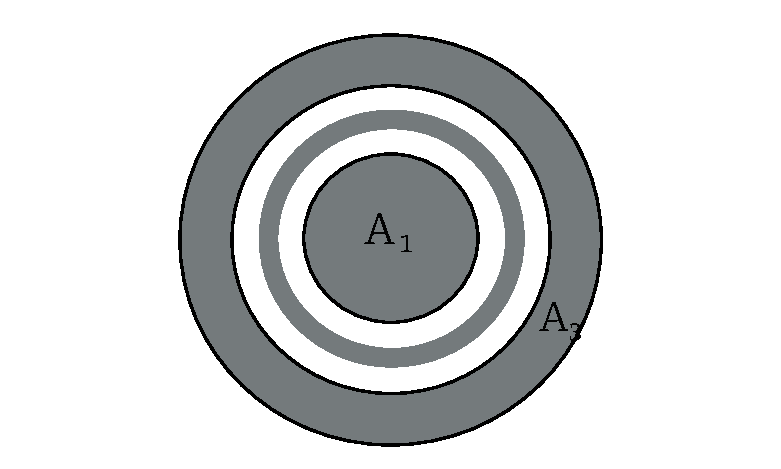
\includegraphics[height=6cm]{images/Capitulo_3/cdc_geometria_top}
        \caption{Vista frontal.}
    \end{subfigure}
    ~ %add desired spacing between images, e. g. ~, \quad, \qquad, \hfill etc. 
      %(or a blank line to force the subfigure onto a new line)
    \begin{subfigure}[b]{0.45\textwidth}
    	\centering
        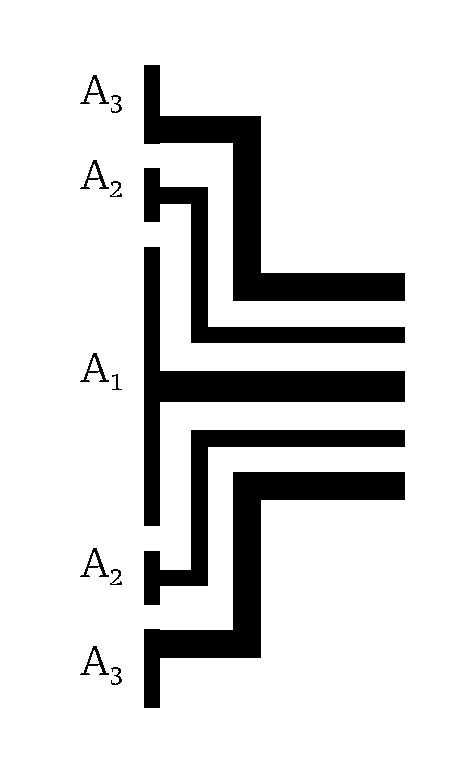
\includegraphics[height=6cm]{images/Capitulo_3/cdc_geometria_side}
        \caption{Vista lateral.}
    \end{subfigure}
    \caption{Geometr�a del SDC}
    \label{fig:geometria-sdc}
\end{figure}

Se define $A_3$ como el �rea del anillo externo $S_3$ y $A_1$ como el �rea de la placa frontal $S_1$. Y a la relaci�n entre estos dos como $\alpha$ de manera que: 

\begin{equation}
\alpha = \frac{A_1}{A_3}
\end{equation}

Si realizamos una simulaci�n variando los par�metros $A_1$ y $A_3$, podemos observar que entre m�s grande sea el �rea del electrodo m�s grande ser� la capacitancia. Este comportamiento concuerda con la ecuaci�n del capacitor de placas paralelas \ref{eq:capacitor-placas-paralelas}.

\begin{equation}
C = \frac{\epsilon A}{d}
\label{eq:capacitor-placas-paralelas}
\end{equation} 

Suponiendo un objetivo de sensado con superficie plana y un �rea total constante $A_t$ el valor de $\alpha$ que maximiza la capacitancia del sensor es igual a $1$, en otras palabras, �reas iguales entre la placa frontal y el anillo exterior \cite{cite_s15_2017_snoa928}.

Sin embargo el rotor es un objetivo con una superficie curva por lo que hay que tener en cuenta los efectos que pueda tener en la sensitividad del sensor. En la figura \ref{fig:grafica_desfasamiento_capacitancia} se puede observar que bajo diferentes curvaturas el valor �ptimo de $\alpha$ se desfasa. 

\begin{figure}[H]
    \centering
    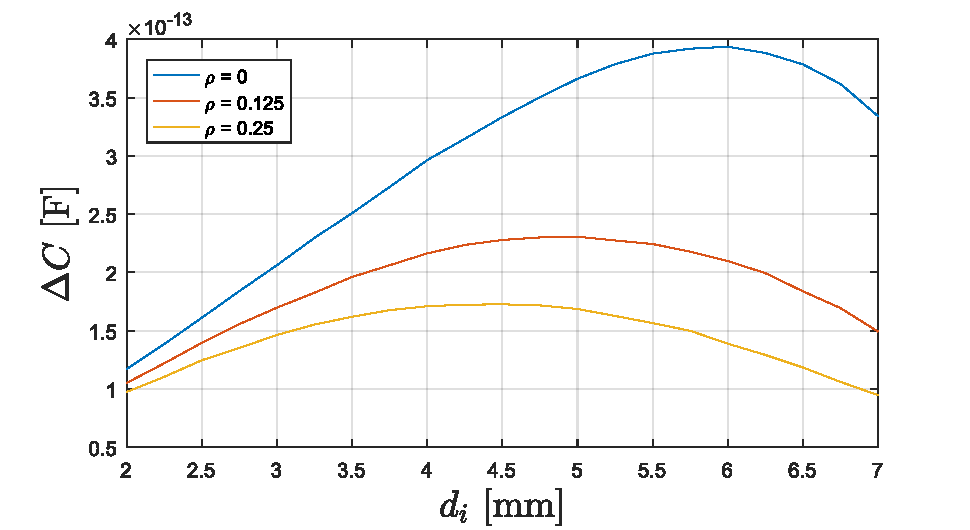
\includegraphics[width=0.8\textwidth]{images/Capitulo_3/grafica_desfasamiento_capacitancia}
    \caption{Desfasamiento de punto �ptimo en el SDC.}
    \label{fig:grafica_desfasamiento_capacitancia}
\end{figure}

Entonces para calcular el punto �ptimo es necesario realizar un conjunto de simulaciones variando $\alpha$, contemplando la curvatura real del rotor. Esto se realiza mediante un script de \textbf{Matlab} capaz de generar diferentes configuraciones del electrodo y ejecutar una simulaci�n en FEMM para calcular la capacitancia dentro de cada configuraci�n. Este conjunto de datos es recolectado y graficado para determinar el punto �ptimo como se muestra en la figura \ref{fig:grafica_capacitancia_optima}.

\begin{figure}[H]
    \centering
    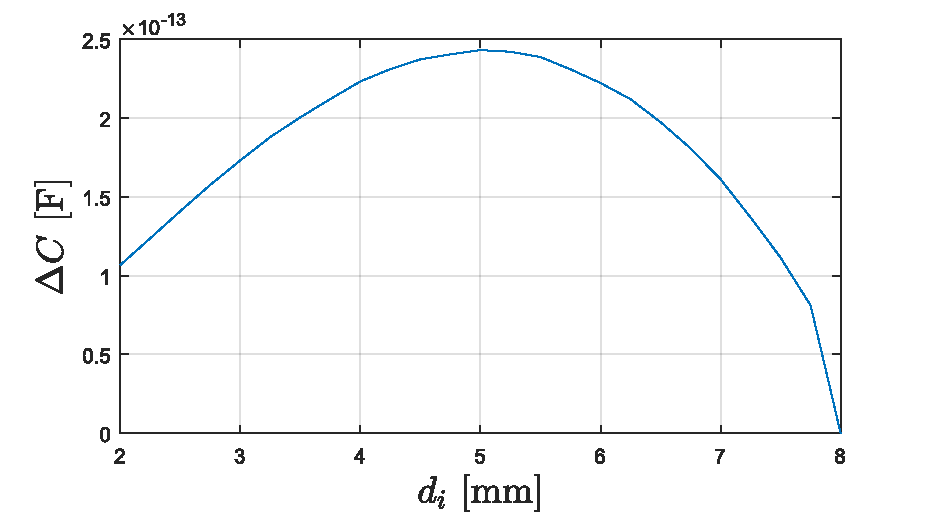
\includegraphics[width=0.8\textwidth]{images/Capitulo_3/grafica_capacitancia_optima}
    \caption{Configuraci�n �ptima del SDC.}
    \label{fig:grafica_capacitancia_optima}
\end{figure}

Finalmente se ejecuta otro script que var�a la distancia entre el objetivo y el sensor para obtener la curva caracter�stica mostrada en la figura \ref{fig:sensor_caracterizacion_final_radial}.

\begin{figure}[H]
    \centering
    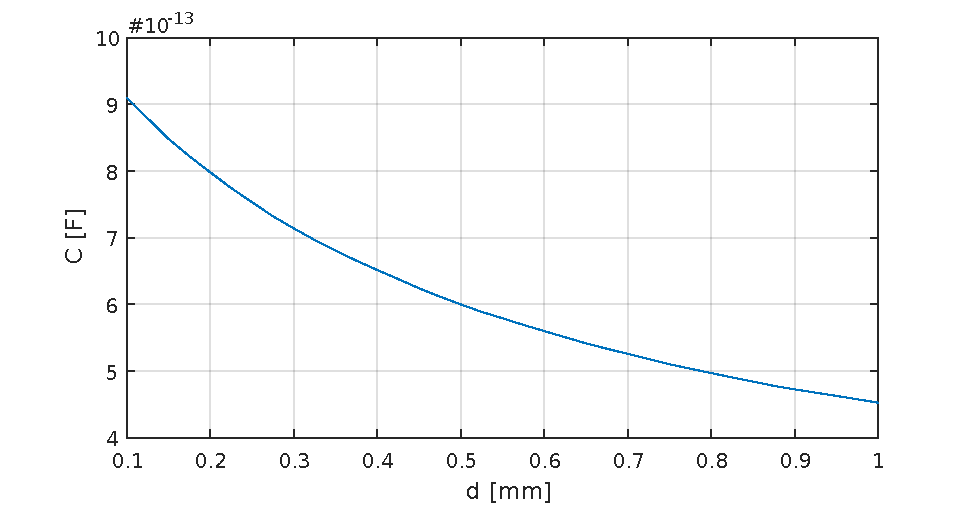
\includegraphics[width=0.8\textwidth]{images/Capitulo_3/sensor_caracterizacion_final_radial}
    \caption{Curva caracter�stica del SDC.}
    \label{fig:sensor_caracterizacion_final_radial}
\end{figure}

\subsection{Circuito de acondicionamiento}

Una vez conocidos el rango de capacitancias es posible dise�ar un circuito que se encargar� de convertir la capacitancia del electrodo en una se�al cuadrada con una frecuencia variable, seguido de la conversi�n de la se�al cuadrada a una se�al diferencial para aumentar su inmunidad al ruido. Este circuito adem�s se encarga de aplicar un voltaje al blindaje activo del electrodo hasta llevarlo al mismo potencial el�ctrico que la placa frontal con el fin de reducir los efectos de la capactitancia par�sita. 

La conversi�n es realizada por un circuito integrado 555 en configuraci�n de multivibrador astable, usando el electrodo como capacitor de temporizaci�n. Este  circuito debe de ser la versi�n CMOS del 555 que presenta menores corrientes de polarizaci�n, las cuales podr�an alterar la frecuencia de oscilaci�n.

El potencial del blindaje activo es controlado por un amplificador operacional en modo seguidor de voltaje, el cual tiene una salida id�ntica al voltaje de su entrada adem�s de una alta impedancia de entrada con el fin de no alterar las mediciones de frecuencia. Adem�s la conversi�n de se�al simple a se�al balanceada es realizada por un driver diferencial.

\begin{figure}[H]
    \centering
    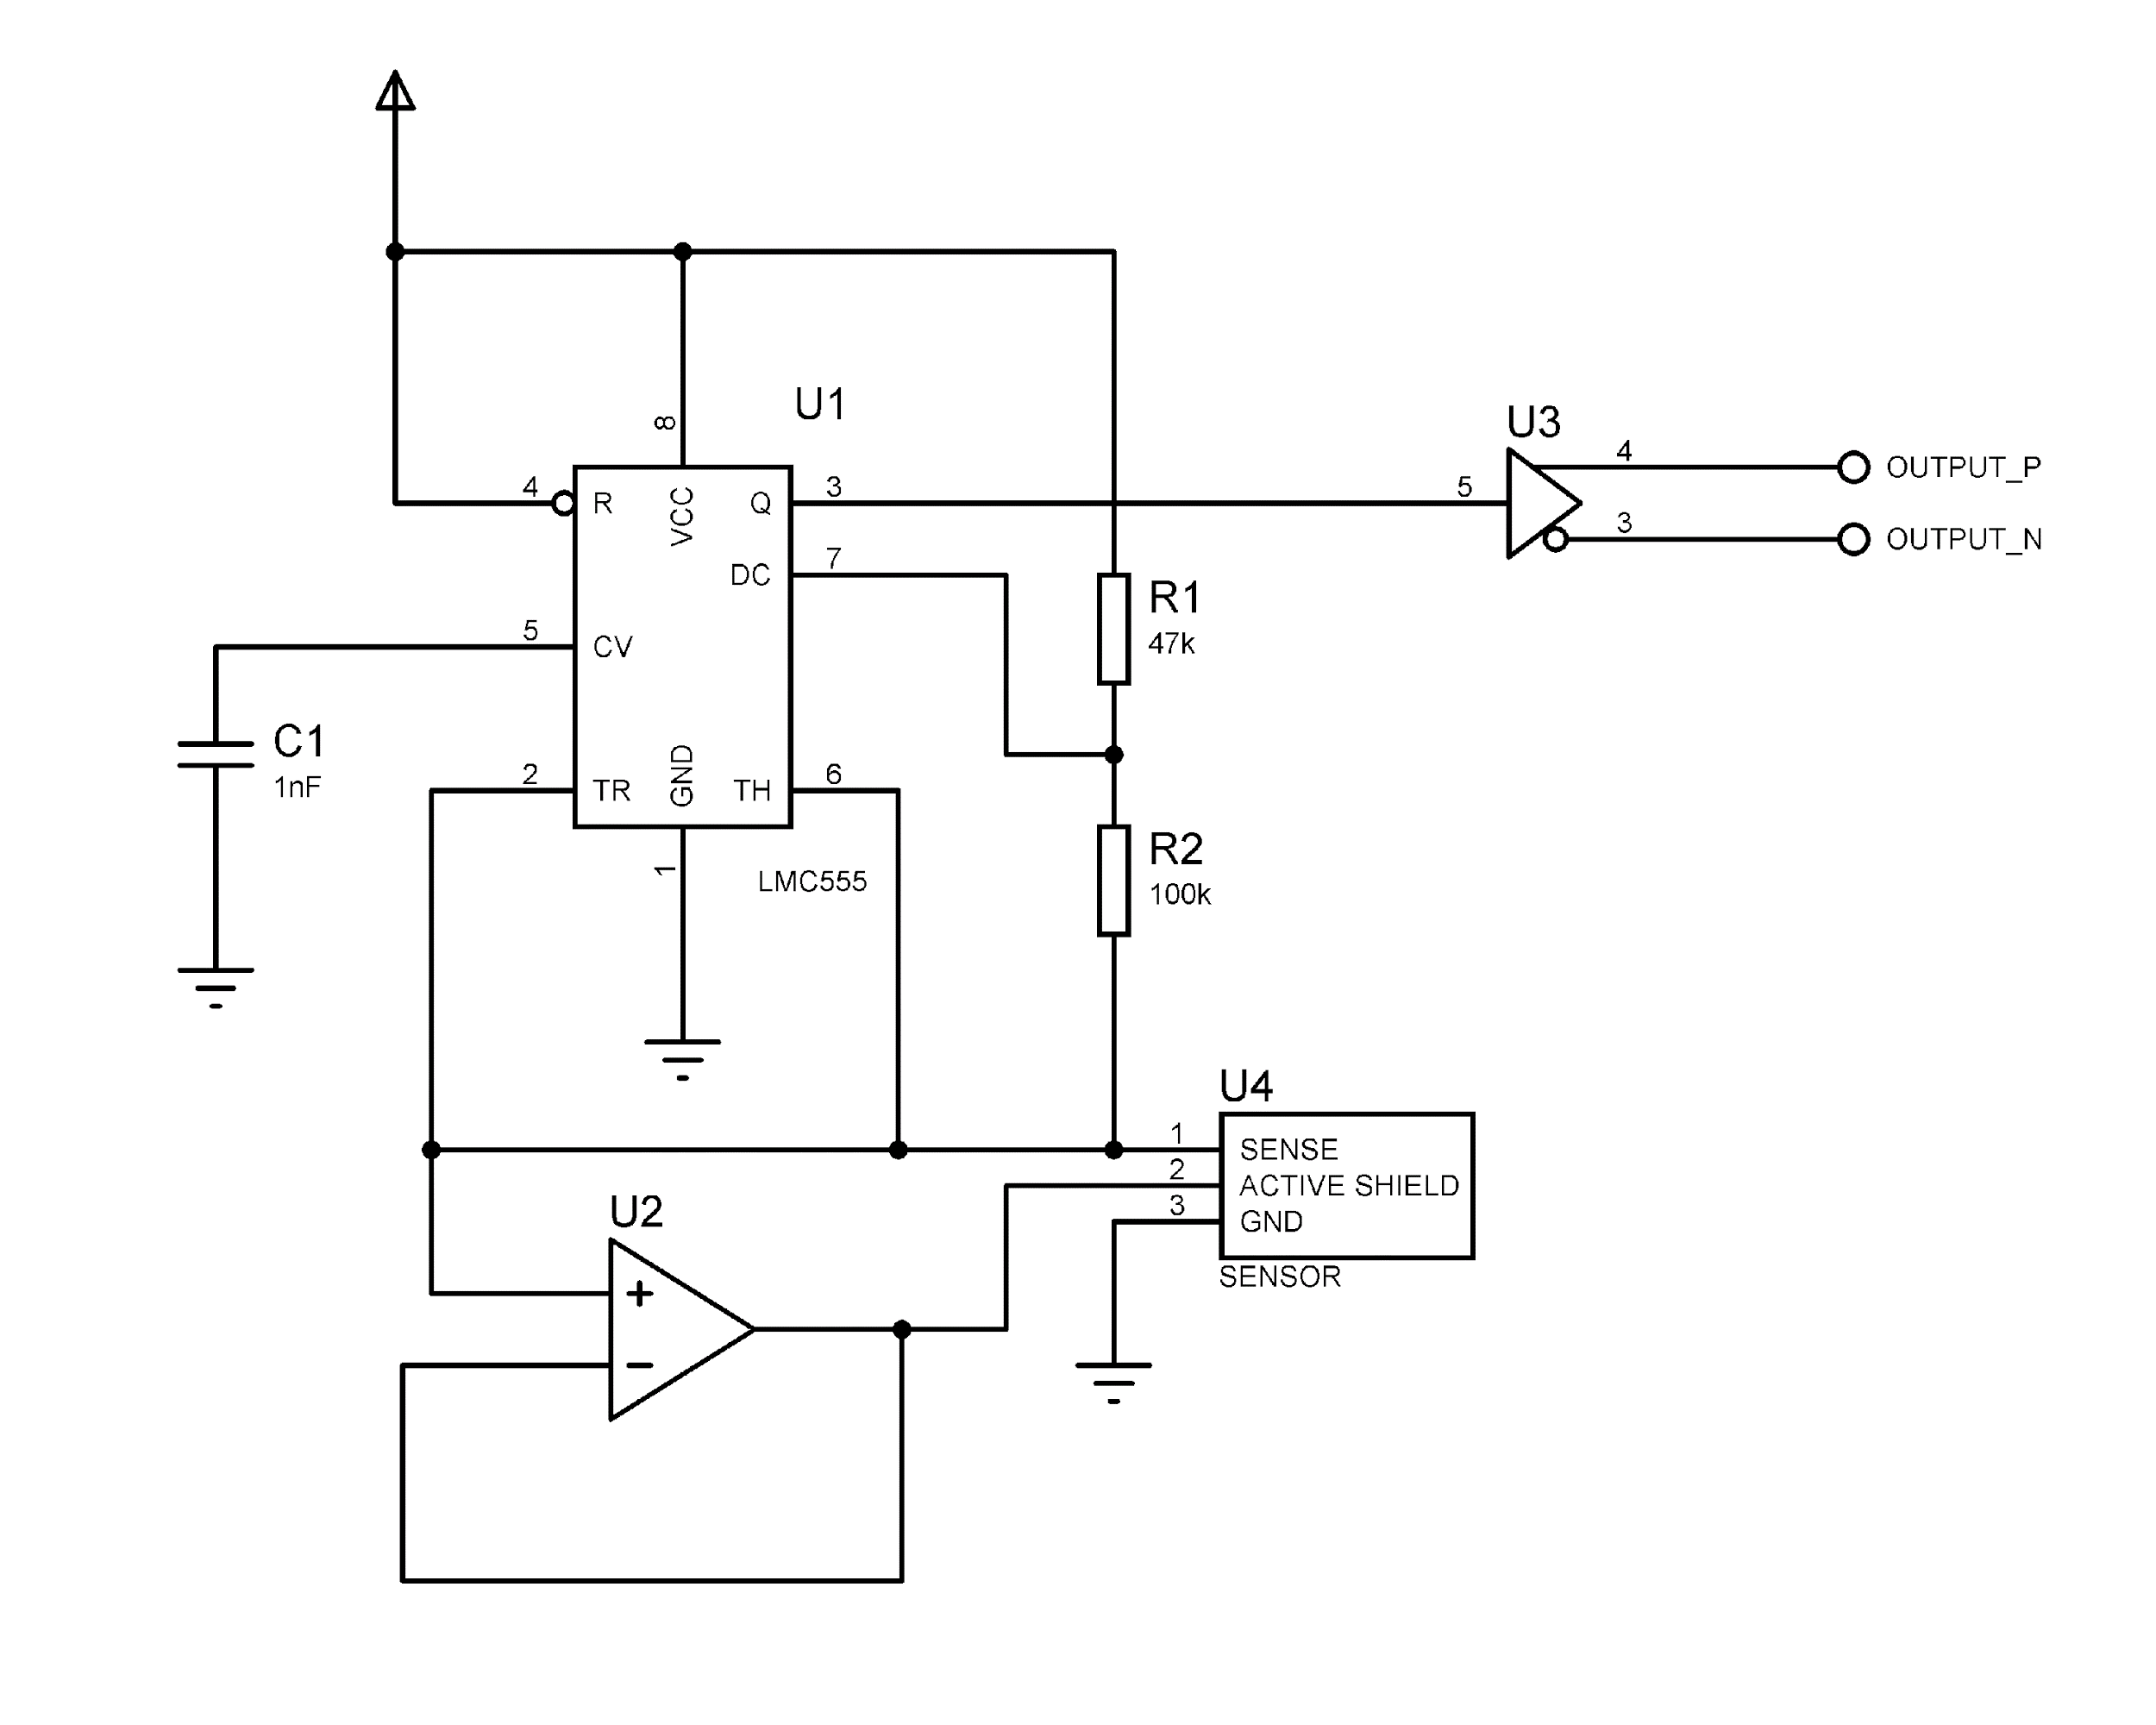
\includegraphics[width=0.8\textwidth]{images/Capitulo_3/Circuito_acondicionamiento}
    \caption{Circuito de acondicionamiento.}
\end{figure}

Finalmente el circuito queda dentro de una caja met�lica a fin de operar como jaula de Faraday y aislarlo del posible ruido el�ctrico en el ambiente como se muestra en la figura \ref{fig:explosionado-sdc}. 

\begin{figure}[H]
    \centering
    \includegraphics[width=0.8\textwidth]{images/Capitulo_3/sdc_ensamble}
    \caption{Explosionado del SDC.}
    \label{fig:explosionado-sdc}
\end{figure}

\newpage

\section{Collar�n de levitaci�n}

Como se mencion� anteriormente, con el prop�sito de lograr la levitaci�n del eje sin importar el material del que est� fabricado, se propuso el uso de un collar�n que sostenga el eje dentro del rodamiento y que cuente con una secci�n de material ferromagn�tico, de manera que sea esta la que interact�e con los electroimanes de los rodamientos activos y con el im�n permanente. 

Este collar�n se compone principalmente de cuatro partes: el cuerpo principal, el anillo ferromagn�tico para el RMR (n�cleo radial) y el MCCE (n�cleo pasivo), el disco de detecci�n y el disco ferromagn�tico para el RMA (n�cleo axial). 

\begin{figure}[H]
    \centering
    \includegraphics[width=0.625\textwidth]{images/Capitulo_3/diagrama_funcional_cl}
    \caption{Diagrama funcional del collar�n de levitaci�n.}
\end{figure}

\newpage

\subsection{Material del anillo y disco ferromag�tico}

Como se realiz� en la secci�n \ref{sec:seleccion-somaloy}, se selecciona el material Somaloy 3P [hoja de datos en anexo D] para formar el anillo y n�cleo ferromagn�ticos. Este material posee las siguientes caracter�sticas: 

\begin{itemize}
\item Punto de saturaci�n: $1.42 - 1.63 T$
\item Permeabilidad relativa: $\mu_r = 950$
\end{itemize}

\subsection{Material del cuerpo principal}

El cuerpo principal se usa como medio de acople entre el collar�n y el eje, adem�s de servir como soporte para el resto de los componentes. Sin embargo, el cuerpo del collar�n cuenta con algunas restricciones en cuanto al material del que est� fabricado:

\begin{itemize}
\item El material no puede ser met�lico para evitar las corrientes par�sitas (corrientes de Foucault).
\item Debe ser lo suficientemente r�gido para evitar deformarse por las fuerzas que act�en sobre �l. 
\item Debe ser lo suficientemente liviano para no exceder la fuerza m�xima que puede generar los electroimanes y el im�n permanente.  
\item Adem�s debe contar con una permitividad el�ctrica ($\epsilon$) alta para mejorar su detectabilidad antes el SDC. 
\end{itemize}

Una de las mejores alternativas que tenemos y que pueden cumplir con estas caracter�sticas son los pol�meros. Los pl�sticos en ingenier�a han tenido una gran aceptaci�n debido a sus caracter�sticas espec�ficas. Poseen buenas propiedades mec�nicas como una gran resistencia al impacto y a la fatiga, bajo coeficiente de fricci�n, resistencia al desgaste y al ataque por sustancias qu�micas, su bajo costo en comparaci�n con la mayor�a de los metales adem�s de ser m�s livianos y m�s f�ciles de maquinar. 

Uno de los pl�sticos de ingenier�a m�s utilizados es el Nylamid, de la familia de las Poliamidas (PA). Debido a sus propiedades mec�nicas y el�ctricas, a su amplia variedad de presentaciones y medidas y a su relativamente bajo costo se ha utilizado mucho para la fabricaci�n de piezas en el ramo industrial sustituyendo materiales como el acero, bronce, aluminio, madera y cer�mica. 

Sin embargo, para tener una mayor certeza en cuanto al material seleccionado se dispuso a utilizar el m�todo gr�fico para la selecci�n de materiales apoy�ndonos en el software CES EduPack. Este m�todo utiliza mapas de materiales, tambi�n denominados diagramas de Ashby. En estos diagramas se puede hacer una aproximaci�n del material m�s adecuado con base en las propiedades m�s importantes que debe poseer el componente. Agrupan los materiales en diferentes familias, formando grupos cerrados y relacionando en pares ciertas propiedades de los materiales. 

Para nuestro caso compararemos dos propiedades relacionadas a las restricciones que se establecieron para el material:

\begin{itemize}
\item M�dulo de Young.
\item Densidad. 
\end{itemize}

Como sabemos, el M�dulo de Elasticidad, tambi�n llamado M�dulo de Young, es un par�metro caracter�stico de un material que indica la relaci�n que existe entre la tensi�n y la correspondiente deformaci�n unitaria en un material sometido a un esfuerzo, y que est� por debajo del l�mite de elasticidad del material. El m�dulo de Young indica la rigidez del material, es decir, la oposici�n de este a ser deformado. Cuanto m�s r�gido sea el material, mayor es su m�dulo de elasticidad. 

Para el an�lisis del material con el software CES EduPack compararemos �nicamente pol�meros relacionando el M�dulo de Young y la densidad, obteniendo un total de 738 materiales disponibles:

\begin{figure}[H]
    \centering
    \includegraphics[width=\textwidth]{images/Capitulo_3/Material1}
    \caption{Diagrama total de materiales (M�dulo de Young vs. Densidad).}
\end{figure}

Para poder reducir el n�mero de materiales desplegados y facilitar la selecci�n podemos definir algunos l�mites dentro de los par�metros que se establecieron. En este caso, nos basaremos en los valores de densidad y m�dulo de Young de las poliamidas que, como ya vimos, son uno de los pl�sticos de ingenier�a m�s utilizados, principalmente para la fabricaci�n de componentes mec�nicos como rodamientos y engranes. 

Esto nos ayuda a establecer un par�metro de selecci�n a falta de contar con datos m�s espec�ficos en cuanto a las condiciones de operaci�n m�s all� de las restricciones que se establecieron anteriormente. Estos datos pueden ser obtenidos dentro de la biblioteca de materiales que contiene el software. Sin embargo, debido a la gran cantidad de compuestos y variantes que presenta este material no puede establecerse un valor exacto, por lo que se proponen unos valores promedio de:

\begin{itemize}
\item 2 GPa para el M�dulo de Young.
\item 1.4 $g/cm^3$ para la densidad. 
\end{itemize}

\begin{figure}[H]
    \centering
    \includegraphics[width=\textwidth]{images/Capitulo_3/Material2}
    \caption{L�mite m�ximo para el m�dulo de Young.}
\end{figure}

\begin{figure}[H]
    \centering
    \includegraphics[width=\textwidth]{images/Capitulo_3/Material3}
    \caption{L�mite m�ximo para la densidad.}
\end{figure}

Como podemos notar, las restricciones en cuanto a la familia de materiales y los valores de densidad y m�dulo de Young redujeron de manera significativa la cantidad de materiales de selecci�n, trat�ndose en su mayor�a de ABS, PET y Polipropilenos. 

El siguiente par�metro que se consider� fue la permitividad el�ctrica del material, que como se estableci� en las especificaciones, se prefiere optar por materiales con un valor $\epsilon$ mayor. Se defini� una permitividad relativa m�nima de $3.5$, el cual corresponde al valor de la permitividad relativa del Nylon \cite{cite_s20_2017_goodfellow}. 

Con este �ltimo par�metro se obtuvo el siguiente diagrama, con un total de 91 materiales de selecci�n posibles de los 738 que se ten�an originalmente: 

\begin{figure}[H]
    \centering
    \includegraphics[width=\textwidth]{images/Capitulo_3/Material4}
    \caption{L�mite m�ximo para el costo del material.}
\end{figure}

Al consultar individualmente las propiedades de los materiales restantes se consigui� encontrar un material que puede utilizarse para la fabricaci�n del collar�n de levitaci�n, debido a sus propiedades y a las aplicaciones para las que normalmente se utiliza. Este material es el Polioximetileno (POM), tambi�n conocido como Acetal [v�ase anexo E]:

\begin{figure}[H]
    \centering
    \includegraphics[width=\textwidth]{images/Capitulo_3/Material5}
    \caption{Identificaci�n del material Acetal (POM).}
\end{figure}

El Acetal se caracteriza por su bajo coeficiente de fricci�n, su resistencia al desgaste y buena resistencia a la abrasi�n, as� como facilidad de maquinado. Tiene alta resistencia a impactos y a la humedad, provee alta resistencia y rigidez en combinaci�n con su excelente estabilidad dimensional y elevado m�dulo de elasticidad.
Se utiliza principalmente para la fabricaci�n de engranes, cojinetes, dispositivos de sujeci�n, ruedas, rodillos, soportes estructurales, etc \citep{cite_s17_2017_prospector_acetal}.

Debido a sus caracter�sticas y aplicaciones se consider� el Acetal (POM) como el material del que se constituir�a el collar�n de levitaci�n ya que cumple con las propiedades necesarias para cubrir las especificaciones que se plantearon inicialmente. 

La segunda pieza que se debe considerar es el disco posterior. Este disco debe su forma a que se utiliza como superficie para medir la posici�n del rotor en la direcci�n axial con ayuda del sensor acoplado al RMA. A modo de simplificaci�n se opt� porque dicho disco se componga del mismo material que el cuerpo principal del collar�n [Acetal (POM)].

El ensamble final de los componentes descritos anteriormente se muestran en la figura \ref{fig:collarin-ensamble}.

\begin{figure}[H]
    \centering
    \includegraphics[width=0.8\textwidth]{images/Capitulo_3/funda_asm}
    \caption{Ensamble final del collar�n de levitaci�n.}
    \label{fig:collarin-ensamble}
\end{figure}

\newpage

\section{Controlador}

Un rodamiento magn�tico no estar�a completo sin un sistema de control que se encarga de hacer las correcciones necesarias para mantener el eje en levitaci�n. Este sistema de control consiste en un controlador retroalimentado en espacio de estados y un observador para determinar el estado del sistema. 

El procedimiento realizado a continuaci�n consiste en obtener un modelo din�mico del eje, linealizar la representaci�n del sistema, especificar la respuesta deseada, calcular las ganancias del controlador-observador en modo continuo y discretizar el conjunto controlador-observador. Adem�s mediante el control calendarizado se compensar�n los efectos de controlar un sistema no lineal usando una aproximaci�n linealizada. Finalmente se discuten los efectos que puede tener el ruido de los sensores y su soluci�n mediante la implementaci�n del observador de Kalman. 

\begin{figure}[H]
    \centering
    \includegraphics[width=0.625\textwidth]{images/Capitulo_3/diagrama_funcional_controlador}
    \caption{Diagrama funcional del controlador.}
\end{figure}

\newpage

\subsection{Modelo din�mico del eje} \label{sec:modelo-dinamico}

El primer paso consiste en obtener el modelo din�mico del sistema. En la figura \ref{fig:diagrama-cl-eje} podemos observar las fuerzas que act�an sobre el eje $F_a$, $F_r$, $F_p$ correspondientes al EIA, EIR e IP respectivamente. 

\begin{figure}[H]
\begin{center}
\centering
\includegraphics[width=\textwidth]{images/Capitulo_2/diagrama_cuerpo_libre_rotor}
\caption{Diagrama de cuerpo libre del eje.}
\label{fig:diagrama-cl-eje}
\end{center}
\end{figure}

El EIR ejerce fuerzas en el plano $Y-Z$, mientras el EIA y el IP ejercen fuerzas en los ejes $X$ y $Z$ respectivamente. Estas fuerzas est�n representadas en la ecuaci�n \ref{eq:fuerzas-rotor}. 

\begin{equation}
	\vec{F}_{r} = \begin{pmatrix}
	0\\
	F_{ry}\\
	F_{rz}\\
	\end{pmatrix}
	\vec{F}_a = \begin{pmatrix}
	F_{ax}\\
	0\\
	0\\
	\end{pmatrix}
	\vec{F}_p = \begin{pmatrix}
	0\\
	0\\
	F_{pz}\\
	\end{pmatrix}
	\label{eq:fuerzas-rotor}
\end{equation}

Los respectivos momentos generados por el EIR y el IP son:

\begin{equation}
	\vec{M}_r = \vec{r}_r \times \vec{F}_r 
\end{equation}

\begin{equation}
	\vec{M}_p = \vec{r}_p \times \vec{F}_p 
\end{equation}

Si consideramos la acci�n conjunta de ambos EIA como una sola fuerza, entonces el momento generado por estos ser� de la forma:

\begin{equation}
	\vec{M}_A = \vec{r}_a \times abs(\vec{F}_a)
\end{equation}

Para establecer la ecuaci�n de suma de momentos es necesario determinar la matriz de inercia para el eje representado por la figura \ref{fig:inercia-rotor-diagrama}. 

\begin{figure}[H]
\begin{center}
\centering
\includegraphics[width=12cm]{images/Capitulo_3/diagrama_momentos}
\caption{Diagrama de momentos de inercia.}
\label{fig:inercia-rotor-diagrama}
\end{center}
\end{figure}

En la figura \ref{fig:inercia-rotor-diagrama} podemos identificar tres elementos correspondientes al eje y al par de collarines. Podemos calcular la matriz de inercia respecto a los ejes principales aplicando el teorema de ejes paralelos, lo que resulta en la ecuaci�n \ref{eq:matriz-inercia-paralelos}. 

\begin{equation}
	[I] = \begin{pmatrix}
	I_{xxa} + 2I_{xxb}  & 0 & 0\\
	0 & I_{yya} + 2I_{yyb} + 2m_b r_b^2 & 0\\
	0 & 0 & I_{zza}+2I_{zzb}+ 2 m_b r_b^2
	\end{pmatrix}
	\label{eq:matriz-inercia-paralelos}
\end{equation}

Debido a que el conjunto eje-collar�n posee simetr�a radial respecto al eje $X$, los momentos principales $Iyy$ e $Izz$ son iguales, lo que permite reducir la ecuaci�n \ref{eq:matriz-inercia-paralelos} a la forma:  

\begin{equation}
	[I] = \begin{pmatrix}
	I_{xx}  & 0 & 0\\
	0 & I_{\rho}  & 0\\
	0 & 0 & I_{\rho}
	\end{pmatrix}
	\label{eq:matriz-inercia-reducida}
\end{equation}

Como indica la secci�n \ref{sec:angulos-euler} es necesario definir un marco de referencia m�vil para establecer las ecuaciones din�mica. Como el cuerpo es axisim�trico solo son necesarias dos rotaciones para describir su orientaci�n, siempre y cuando permitamos la libre rotaci�n (spin) dentro de este nuevo marco de referencia. Estas corresponden a las primeras dos rotaciones extr�nsecas Tait-Bryan $z-y-x$ como se muestra en la figura \ref{fig:angulos-tb-2}. 

\begin{figure}[H]
\begin{center}
\centering
\includegraphics[width=8cm]{images/Capitulo_2/angulos_euler_rotor}
\caption{Marco de referencia m�vil.}
\label{fig:angulos-tb-2}
\end{center}
\end{figure}

Podemos definir este nuevo marco de referencia como la transformaci�n $T_O^B$ como se muestra en la ecuaci�n:

\begin{equation}
	T_O^B (\theta,\psi)= {T_A}^B (\theta) {T_A}^O (\psi) 	
	\label{eq:transformada-marco-movil}
\end{equation}

Donde las matrices de rotaci�n ${T_A}^B (\theta)$ y ${T_A}^O (\psi)$ est�n definidas en la ecuaci�n \ref{eq:matrices-angulos-euler}, y como el eje gira dentro del eje $X$ del marco de referencia m�vil con una velocidad $\omega_\phi$, la velocidad angular $\omega$ del eje estar� descrita por:

\begin{equation}
  \omega = \omega_\phi + \Omega
\end{equation}

Donde $\Omega$ es la velocidad angular del marco de referencia m�vil. Calcular el producto cruz de la ecuaci�n \ref{eq:derivada-inercia-coriolis} requiere que ambos vectores est�n en el mismo marco de referencia. Por lo que es necesario transformar los vectores de fuerza al marco m�vil mediante la matriz de transformaci�n $T^{B}_O$.

La ecuaci�n \ref{eq:angulos-intrinsecos-marco-movil} relaciona la variaci�n de los �ngulos intr�nsecos $\phi$ y $\theta$ con la velocidad angular del marco de referencia m�vil respecto al marco fijo $\Omega$. 

\begin{equation}
	\begin{pmatrix}
	\dot{\theta}\\
	\dot{\psi}
	\end{pmatrix} = \begin{pmatrix}
	0 & cos(\phi) & -sin(\phi)\\
	0 & - sin(\phi)sec(\theta) & cos(\phi)sec(\theta)
	\end{pmatrix} \begin{pmatrix}
	\Omega_x\\
	\Omega_y\\
	\Omega_z
	\end{pmatrix}
	\label{eq:angulos-intrinsecos-marco-movil}
\end{equation}

Sustituyendo los t�rminos descritos en la secci�n \ref{sec:modelo-dinamico} en la ecuaci�n \ref{eq:derivada-inercia-coriolis} se obtiene el sistema de ecuaciones \textbf{[sistema de ecuaciones]}. 

\textbf{[instertar ecuacion espacio de estados del sistema]} 

Estas ecuaciones se introducen dentro del modelo de \textbf{Simulink} mostrado en la figura \ref{fig:modelo-sistema} para realizar la simulaci�n.   

\begin{figure}[H]
\begin{center}
\centering
\includegraphics[width=\textwidth]{images/Capitulo_3/Control_SIMULINK_MATLAB/modelo_simulink_sistema}
\caption{Modelos del sistema.}
\label{fig:modelo-sistema}
\end{center}
\end{figure}

\subsection{Linealizaci�n}

Podemos observar que este sistema de ecuaciones es no lineal, as� que tenemos que linealizarlo para convertirlo en la forma can�nica de espacio de estados, y aplicar las t�cnicas de control descritas en la secci�n \ref{sec:control} mediante las f�rmulas \ref{eq:control:jacobiano}. 

[..............]

Lo que resulta en el sistema descrito por las matrices:

[..............]

\subsection{Controlador}

Con el fin de estabilizar el sistema descrito en la ecuaci�n \textbf{[sistema linealizado]} utilizamos el esquema de control retroalimentado presentado en la secci�n \ref{sec:control-retroalimentado}. 

Se selecciona un conjunto de polos para el nuevo sistema y se utiliza el script de \textbf{Matlab}\textbf{[anexo]} para calcular las ganancias del controlador $K$. Este esquema de control es implementado en el modelo de \textbf{Simulink} mostrado en la figura \ref{fig:esquema-controlador-retroalimentado}. 

\begin{figure}[H]
\begin{center}
\centering
\includegraphics[width=.7\textwidth]{images/Capitulo_3/Control_SIMULINK_MATLAB/controlador_retroalimentado}
\caption{Esquema del controlador retroalimentado.}
\label{fig:esquema-controlador-retroalimentado}
\end{center}
\end{figure}

El esquema de control mostrado anteriormente es capaz de estabilizar el sistema pero no puede alcanzar un error de estado estable igual a $0$, por lo que se agrega un integrador y un vector de ganancias con el fin de producir un nuevo esquema como el mostrado en la secci�n \ref{sec:control-integral}. Este nuevo vector de ganancias es calculado por el \textbf{script [...]} y su modelo de Simulink es el que se muestra en la figura \ref{fig:esquema-controlador-integral}.

\begin{figure}[H]
\begin{center}
\centering
\includegraphics[width=.8\textwidth]{images/Capitulo_3/Control_SIMULINK_MATLAB/controlador_integral}
\caption{Esquema del controlador integral.}
\label{fig:esquema-controlador-integral}
\end{center}
\end{figure}

\subsection{Observador}

Para realizar control en espacio de estados es necesario retroalimentar el estado completo del sistema. En el caso del RMH no se puede medir de manera directa todo los par�metros del vector de estados por lo que es necesario un observador de estados como es descrito en la secci�n \ref{sec:observador-estados}. 

Las ganancias del observador de estados $K_o$ son calculadas mediante el\textbf{ script [...]}. El modelo de \textbf{Simulink} correspondiente a este observador es mostrado en la figura \ref{fig:esquema-observador-estados}.

\begin{figure}[htb]
\begin{center}
\centering
\includegraphics[width=.85\textwidth]{images/Capitulo_3/Control_SIMULINK_MATLAB/observador_de_estados}
\caption{Esquema del observador de estados.}
\label{fig:esquema-observador-estados}
\end{center}
\end{figure}

\subsection{Discretizaci�n}

Debido a que los controladores suelen ser implementados en un sistema digital, es necesario contar con una versi�n discreta de los controladores presentados anteriormente.  

Como se indica en la secci�n \ref{sec:discretizacion-controladores}, para emular un sistema controlador-observador es necesario transformar los polos que definen la respuesta del sistema del dominio de Laplace al dominio de $Z$. Esto se realiza mediante la transformaci�n de Tustin expresada en la ecuaci�n \ref{eq:ecuacion-Tustin}.

Para el c�lculo de las ganancias del controlador discreto, es necesario discretizar el sistema continuo y, con el nuevo conjunto de polos discretos, aplicar las t�cnicas de ubicaci�n de polos descritas en la secci�n \ref{sec:discretizacion-controladores}. 

Los modelos continuos presentados anteriormente son discretizados y presentados en las figuras \ref{fig:esquema-controlador-discreto} y \ref{fig:esquema-observador-discreto}. Cabe resaltar que lo que era un integrador en el sistema continuo ahora es un acumulador en lugar de un retardo unitario ($Z^{-1}$).  

\begin{figure}[htb]
\begin{center}
\centering
\includegraphics[width=.85\textwidth]{images/Capitulo_3/Control_SIMULINK_MATLAB/controlador_discreto}
\caption{Esquema del controlador discreto.}
\label{fig:esquema-controlador-discreto}
\end{center}
\end{figure}

\begin{figure}[H]
\begin{center}
\centering
\includegraphics[width=.85\textwidth]{images/Capitulo_3/Control_SIMULINK_MATLAB/observador_discreto}
\caption{Esquema del observador discreto.}
\label{fig:esquema-observador-discreto}
\end{center}
\end{figure}

\subsection{Control calendarizado}

Con el fin de compensar los efectos de las no linealidades provocadas por la precesi�n del eje utilizamos el m�todo de control calendarizado descrito en la secci�n \ref{sec:control-calendarizado}, en donde linealizamos en diferentes valores de $\Omega$ para obtener el conjunto de matrices de transici�n $A$, $B$, $C$ y el conjunto de ganancias $K$ y $K_o$ para el observador de estados. Estos c�lculos son realizados por el \textbf{script [...]} y el conjunto de matrices es interpolado durante la simulaci�n del modelo de \textbf{Simulink} mostrado en las figuras \ref{fig:esquema-controlador-calendarizado} y \ref{fig:esquema-observador-calendarizado} . 

%\textbf{[insertar modelo simulink]}

\begin{figure}[htb]
\begin{center}
\centering
\includegraphics[width=.9\textwidth]{images/Capitulo_3/Control_SIMULINK_MATLAB/controlador_caliderizado_discreto}
\caption{Esquema del controlador calendarizado.}
\label{fig:esquema-controlador-calendarizado}
\end{center}
\end{figure}
 \newpage
\begin{figure}[t!]
\begin{center}
\centering
\includegraphics[width=.85\textwidth]{images/Capitulo_3/Control_SIMULINK_MATLAB/observador_calendarizado}
\caption{Esquema del observador calendarizado.}
\label{fig:esquema-observador-calendarizado}
\end{center}
\end{figure}

\subsection{Observador de Kalman}

Si el ruido en los sensores alcanza niveles excesivos la estabilidad del controlador podr�a verse comprometida, por motivos de seguridad es necesario contar con un sistema m�s robusto en cuanto a inmunidad al ruido. Esto puede alcanzarse mediante el filtro de Kalman. 
 
El filtro de Kalman es un observador en tiempo discreto que permite mejorar la calidad de nuestras mediciones gracias a que incorpora informaci�n sobre la din�mica del sistema y los niveles de ruido (covarianza) presente en las mediciones de los sensores. En el caso del rodamiento magn�tico se a�ade la ventaja de que integra la informaci�n redundante de los tres sensores de posici�n radial. 

A partir del sistema discretizado se aplican las f�rmulas del filtro de Kalman descritas en la secci�n \ref{sec:filtro-kalman}. Cabe resaltar que las ganancias del filtro de Kalman son calculadas en l�nea y de manera iterativa, a diferencia de las ganancias del observador cl�sico. 

%El filtro queda implementado en el modelo de \textbf{Simulink} mostrado en la \textbf{figura [...]}. 

%\textbf{[insertar modelo de simulink]}

%%%%%%%%%%%%%%%%%%%%%%%%%%%%%%%%%%%%%%%%%%%%%%%%%%%%%%%%%%%%%%%%%%%
%%%%%%%%%%%%%%%%%%%%%%%%%%%%%%%%%%%%%%%%%%%%%%%%%%%%%%%%%%%%%%%%%%%
%%%%%%%%%%%%%%%%%%%%%%%%%%%%%%%%%%%%%%%%%%%%%%%%%%%%%%%%%%%%%%%%%%%
%%%%%%%%%%%cccccccccc33333333%%%%%%%%%%%%%%%%%%%%%%%%%%%%%%%%%%%%%%
\chapter{Validaci�n y An�lisis de Resultados}\index{Validaci�n}




%%%%%%%%%%%%%%%%%%%%%%%%%%%%%%%%%%%%%%%%%%%%%%%%%%%%%%%%%%%%%%%%%%%
%%%%%%%%%%%%%%%%%%%%%%%%%%%%%%%%%%%%%%%%%%%%%%%%%%%%%%%%%%%%%%%%%%%
%%%%%%%%%%%%%%%ccccccccccccccccc44444444444444444%%%%%%%%%%%%%%%%%
%%%%%%%%%%%%%%%%%%%%%%%%%%%%%%%%%%%%%%%%%%%%%%%%%%%%%%%%%%%%%%%%%%%
%%%%%%%%%%%%%%%%%%%%%%%%%%%%%%%%%%%%%%%%%%%%%%%%%%%%%%%%%%%%%%%%%%%
\chapter{Conclusiones}
%\todo[inline]{Efectos de control el rotor en 3d}
%%\todo[inline]{Modelar en 3d mejora el desempe\~no del controlador}
%%\todo[inline]{pero esto requirio un modelo mas complejo y la implemetacion de un control calendarizado}
%%\todo[inline]{Efectos del en sistema hibrido}
%%\todo[inline]{El uso del iman permanente permitio reducir de manera considerable el consumo del rodamiento, inluso ante cargas de baja frecencia}

%%\todo[inline]{Aplicaciones futuras}
%%\todo[inline]{El software de simulacion y la teoria desarroda permitira el rapido desarrolo de electroimanes}
%%\todo[inline]{El sensor de capacitancia tiene aplicaciones por separado}
%%\todo[inline]{Los cualidadesdel sistema hibrido pueden exterse a futuros projectos donde el bajo consumo sea importante, ejemplo un riel de levitacion magnetica para el transporte de carga}

La investigaci\'on mostr\'o una gran cantidad de trabajos e investigaciones sobre los rodamientos magn\'eticos,  cada uno mostraba diferentes propuestas, de las cuales, la idea predominante era sobre los rodamientos magn\'eticos radiales. Aunque se analizaron varias fuentes, ninguna de las consultadas mostr\'o una implementaci\'on de rodamientos magn\'eticos activos (tanto radial como axial) aplicando en conjunto un campo magn\'etico base para la levitaci\'on por medio de imanes permanentes, que en particular fue la propuesta sugerida. El estudio sobre el campo permiti\'o que se lograran resolver las problem\'aticas que se presentaron a lo largo del proyecto. 

Las etapas de dise\~no fueron implementadas bas\'andose en la teor\'ia estudiada, quedando en libertad el equipo el modo de proceder, dado que en las fuentes citadas no se encontraron expl\'icitamente procedimentos estandarizados para el desarrollo de electroimanes.

Se valid\'o el dise\~no realizado mediante el uso del software FEM y gracias a ello, podemos afirmar la validez de nuestro proceso en las geometr\'ias de electroim\'an radial y axial usadas.

Las condiciones de ruido magn\'etico que existen en los RMA, adem\'as de las condiciones de operaci\'on (distancia y resoluci\'on) crearon un problema al momento de seleccionar el sensor de distancia. Despu\'es del estudio y comparaci\'on realizado entre distintos sensores, encontramos a los de tipo capacitivo como la mejor opci\'on para esta aplicaci\'on.

El dise\~no de sensores capacitivos supuso un problema, ya que encontrar una geometr\'ia que maximice la sensitividad requiere el modelado de la capacitancia en geometr\'ias poco convencionales. Solucionamos esto mediante simulaciones electroestáticas y variaciones de los par\'ametros del modelo, con lo que se lleg\'o a una geometr\'ia funcional para un tama\~no de electrodo determinado.

En los inicios del proyecto, el flujo marginal introdujo errores para el c\'alculo de electroimanes; al integrar el modelo de este flujo, se obtuvieron c\'alculos que coinciden con las simulaciones FEM.

Aunque el software FEMM s\'olo sirve para calcular modelos fijos, fue posible usar el enlace con MATLAB para caracterizar las respuestas de los electroimanes, imanes pasivos y sensores.

El sistema no lineal que representa al rotor del rodamiento requiri\'o de una linearizaci\'on para aplicar las t\'ecnicas de control retroalimentado convencional. Sin embargo, un controlador basado en un modelo linearizado sencillo presenta problemas de estabilidad ante las diferentes velocidades angulares a las que puede ser sometido. Este problema fue solucionado mediante la aplicaci\'on de un controlador calendarizado.

En cuanto al control de la posici\'on, se observ\'o la superioridad del control integral para controlar la posici\'on del eje, alcanzando un error a estado estable igual a cero.

Tambi\'en se discretiz\'o el controlador y observador para permitir su implementaci\'on en dispositivos digitales. Las simulaciones demostraron la correcta emulaci\'on del controlador continuo por parte del discreto.

Gracias a las simulaciones de accionamiento h\'ibrido, se mostr\'o que el uso de un im\'an permanente y un mecanismo de retracci\'on (MCCE) elimina la componente constante en la fuerza ejercida por los electroimanes, y por lo tanto, la magnitud de corriente consumida.

Es prudente mencionar que son necesarios avances en cuanto a materiales ferromagn\'eticos, pues los materiales actuales carecen de las propiedades requeridas. Esto obstaculiza el desarrollo de electroimanes potentes y de alta eficiencia. Sin embargo, dados los alcances logrados durante la realizaci\'on del proyecto, es posible darle continuidad desarrollando en trabajos posteriores un prototipo, optimizando el dise\~no al implementar metodolog\'ias como el Dise\~no para la Manufactura (DFM) y el Dise\~no para el Ensamble (DFA). Esto claro, implicar\'ia un an\'alisis m\'as completo para la selecci\'on de materiales y de procesos de manufactura que requerir\'ian cada uno de sus componentes. 
%%%%%%%%%%%%%%%%%%%%%%%%%%%%%%%%%%%%%%%%%%%%%%%%%%%%%%%%%%%%%%%%%%%%%%%%%%%%%%%%%%%%
\newpage
%%%%%%%%%%%%%%%%%%%%%%%%%%%%%%%%%%%%%%%%%%%%%%%
%%%%%%%%%%%%%%%%%%%%%%%%%%%%%%%%%%%%%%%%%%%%%%%%%%%%%%%%%%%%%%%%%%%%%%%%%%%%%%%%%%%%%%
%%%%%%%%%%%%%%%%%%%%%%%%%%%%%%%  BIBLIOGRAFIA  %%%%%%%%%%%%%%%%%%%%%%%%%%%%%%%%%%%%%%%
%%%%%%%%%%%%%%%%%%%%%%%%%%%%%%%%%%%%%%%%%%%%%%%%%%%%%%%%%%%%%%%%%%%%%%%%%%%%%%%%%%%%%%
\bibliographystyle{plain} \nocite{*}
 \bibliography{xbiblioteca}
%%%%%%%%%%%%%%%%%%%%%%%%%%%%%%%%%%%%%%%%%%%%%%%%%%%%%%%%%%%%%%%%%%%%%%%%%%%%%%%%%
%%%%%%%%%%%%%%%%%%%%%%%%%%%%  INDICE  %%%%%%%%%%%%%%%%%%%%%%%%%%%%%%%%%%%%%%%%%%%%
%%%%%%%%%%%%%%%%%%%%%%%%%%%%%%%%%%%%%%%%%%%%%%%%%%%%%%%%%%%%%%%%%%%%%%%%%%%%%%%%%%
%%%%%%%%%%%%%%%%%%%%%%%%%    APENDICES  %%%%%%%%%%%%%%%%%%%%%%%%%%%%%%%%%%%%
\part{Ap�ndices}
\appendix
\chapter{Der erste Anhang (Ap\'endice)}

Das Appendix (Anhang) Fragment wird einmal an der gew\"{u}nschten Position
im Dokument eingef\"{u}gt. Weitere Anh\"{a}nge k\"{o}nnen dann mittels der
Zuweisung von Abschnitten (sections) erzeugt werden.

\bigskip

Ab hier beginnt der \verb|backmatter|.

\chapter{Plano del Ensamble de un \'Area Funcional}

\newpage

\begin{figure}[t]
\centering
	\includegraphics[width=\textheight, height=\textwidth, angle=270]{images/Apendices/Plano_EIR}
	%\caption{\textit{Diagrama Funcional.}}
\end{figure}
\chapter{Plano del Ensamble Final}

\newpage

\begin{figure}[t]
\centering
	\includegraphics[width=\textheight, height=\textwidth, angle=270]{images/Apendices/Plano_Ensamble}
	%\caption{\textit{Diagrama Funcional.}}
\end{figure}
\part{Anexos}
\anexo
\chapter{Rosca m\'etrica ISO-M}

\newpage

\includepdf[pages=2, scale=.9]{images/Anexos/Anexo-Rosca}

\chapter{Hoja de datos Imanes Neodimio-Hierro-Boro}

\newpage

\includepdf[pages=1, scale=.9]{images/Anexos/Anexo-Iman}

\chapter{Caracter\'isticas de Material Ferrita Mn-Zn PC90}

\newpage

\includepdf[pages=6, scale=.9]{images/Anexos/Anexo-Ferrita-PC90}

\backmatter
\newpage
\addcontentsline{toc}{chapter}{\'Indice Alfab\'etico}%
\printindex%
\end{document}
%%%%%%%%%%%%%%%%%%%%%%%%%%%%%%%%%%%%%%%%%%%%%%%%%%%%%%%%%%%%%%%%%%%%%%%%%%%%%%%%%% 